% Don't modify this section unless you know what you're doing!
\documentclass[letterpaper,12pt]{article}
% \usepackage{url}
% \usepackage[nottoc,notlot,notlof]{tocbibind}

\usepackage{tabularx} % extra features for tabular environment
\usepackage{amsmath,amsthm,amssymb}  % improve math presentation
\usepackage{amsmath}
\usepackage{amsfonts}
\usepackage{amssymb}
\usepackage{graphicx} % takes care of graphic including machinery
\usepackage[margin=0.8in,letterpaper]{geometry} % decreases margins
% \usepackage{cite} % takes care of citations
% \usepackage[final]{hyperref} % adds hyper links inside the generated pdf file
\usepackage[english]{babel}
\usepackage{caption}
\usepackage{float}
\usepackage[table]{xcolor}
\usepackage{array}
\usepackage{algorithm}
\usepackage{algpseudocode}
\usepackage{cases}
\usepackage{titlesec}
\usepackage{tikz}
\usepackage[utf8]{inputenc}
\usepackage[T1]{fontenc}
\usepackage{bm}
\usepackage{mathtools}
\usepackage{extarrows}
\usepackage{booktabs} 
\usepackage{dsfont}
\usepackage{authblk}

\usepackage{hyperref}
\usepackage{parskip}

\usepackage[
backend=biber,
style=numeric,
sorting=nty
]{biblatex}
\usepackage{csquotes}


\addbibresource{bibou.bib} %Imports bibliography file




\newtheorem{theorem}{Theorem}
\newtheorem{lemma}{Lemma}
\newtheorem{proposition}{Proposition}
\newtheorem{corollary}{Corollary}
\newtheorem{definition}{Definition}
\newtheorem{example}{Example}
\newtheorem{property}{Property}
\newtheorem{remark}{Remark}

\usepackage{microtype}      % microtypography
\usepackage{lipsum}
\usepackage{nicefrac}
\usepackage{fancyhdr}       % header

 \renewcommand{\algorithmiccomment}[1]{\##1}

\author[1]{El-Mehdi Mehiri\thanks{mehiri314@gmail.com}}
\author[2]{Saad Mneimneh}
\author[1]{Hacène Belbachir}

\affil[1]{\small USTHB,
Faculty of Mathematics,
RECITS Laboratory,
16111 Bab Ezzouar, Algiers,
Algeria}
\affil[2]{Department of Computer Science, Hunter College, The City University of New York, 695 Park Avenue, New York, NY 10065, USA}




% \author{
%  El-Mehdi Mehiri \\
%   Department of Mathematics and Industrial Engineering,\\
%   Polytechnique Montréal, Université de Montréal, \\
%     2900 Boulevard Edouard-Montpetit, QC H3T 1J4,\\
%     Montreal, Canada.\\
%   \texttt{elmehdi.mehiri@polymtl.ca} \\
%   \texttt{mehiri314@gmail.com} \\
%   %% examples of more authors
% }
\title{\textbf{The Towers of Fibonacci, Lucas, Pell, and Jacobsthal}}

\date{}
%++++++++++++++++++++++++++++++++++++++++

\begin{document}
 
	\maketitle
	\begin{abstract} 
We present in this paper four new variants of the Tower of Hanoi problem,  the optimal solution of each of these variants is related to one of the four known numbers Fibonacci, Lucas, Pell, and Jacobsthal. We give an optimal solution to each of these variants, and we present their associated graphs. 
	\end{abstract}

 


\section{Introduction}

Since its invention in 1883 by the French mathematician Édouard Lucas \cite[pp. 55–59]{1}, the problem of the Tower of Hanoi has been one of the most famous problems used to introduce the concept of mathematical induction. 


The original  Tower of Hanoi problem is stated as follows. 
Consider three pegs $1$, $2$, and $3$, called respectively,  source peg, middle peg, and destination peg; and $n\geq 1$ discs of distinct diameters. Initially, all discs are stacked onto the first peg (the source) ordered by their diameters, with the smallest one on top and the largest one on the bottom. The goal is to transfer the $n$ discs to the third peg (the destination), as it is illustrated in Figure \ref{fig:init-final_states}, using the minimum number of moves, and respecting the following rules:

\begin{itemize}
\item[$(r_{1})$] at each step only one disc can be moved;
       \item[$(r_{2})$] the disc moved must be a topmost disc;
       \item[$(r_{3})$] a disc cannot reside on a smaller one.
\end{itemize}

\begin{figure}[H]
    \centering
    

\tikzset{every picture/.style={line width=0.75pt}} %set default line width to 0.75pt        

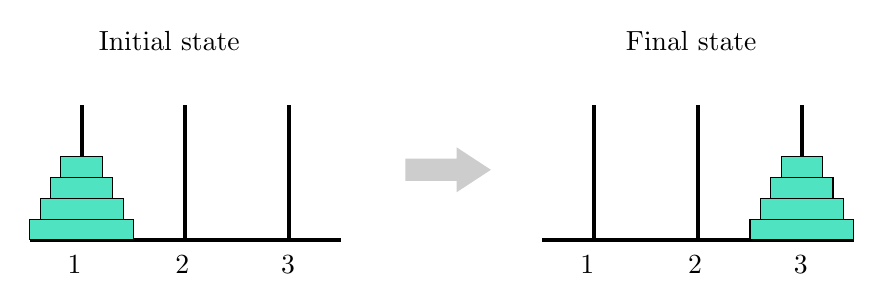
\begin{tikzpicture}[x=0.75pt,y=0.75pt,yscale=-1,xscale=1]
%uncomment if require: \path (0,265); %set diagram left start at 0, and has height of 265

%Straight Lines [id:da47303320704215723] 
\draw [line width=1.5]    (203,153) -- (203,88) ;
%Straight Lines [id:da2596274943436139] 
\draw [line width=1.5]    (253,153) -- (253,88) ;
%Straight Lines [id:da6158417047874292] 
\draw [line width=1.5]    (153,153) -- (153,88) ;
%Straight Lines [id:da5552650208095853] 
\draw [line width=1.5]    (128,153) -- (278,153) ;
%Shape: Rectangle [id:dp7871559520719595] 
\draw  [fill={rgb, 255:red, 80; green, 227; blue, 194 }  ,fill opacity=1 ] (143,113) -- (163,113) -- (163,123) -- (143,123) -- cycle ;
%Shape: Rectangle [id:dp16971724332757798] 
\draw  [fill={rgb, 255:red, 80; green, 227; blue, 194 }  ,fill opacity=1 ] (138,123) -- (168,123) -- (168,133) -- (138,133) -- cycle ;
%Shape: Rectangle [id:dp543708016051085] 
\draw  [fill={rgb, 255:red, 80; green, 227; blue, 194 }  ,fill opacity=1 ] (133,133) -- (173,133) -- (173,143) -- (133,143) -- cycle ;
%Shape: Rectangle [id:dp0244026959370931] 
\draw  [fill={rgb, 255:red, 80; green, 227; blue, 194 }  ,fill opacity=1 ] (128,143) -- (178,143) -- (178,153) -- (128,153) -- cycle ;

%Straight Lines [id:da7221147779404855] 
\draw [line width=1.5]    (450,153) -- (450,88) ;
%Straight Lines [id:da7874597275294666] 
\draw [line width=1.5]    (500,153) -- (500,88) ;
%Straight Lines [id:da4225603478965123] 
\draw [line width=1.5]    (400,153) -- (400,88) ;
%Straight Lines [id:da3778502666400989] 
\draw [line width=1.5]    (375,153) -- (525,153) ;
%Shape: Rectangle [id:dp10843492640608887] 
\draw  [fill={rgb, 255:red, 80; green, 227; blue, 194 }  ,fill opacity=1 ] (490,113) -- (510,113) -- (510,123) -- (490,123) -- cycle ;
%Shape: Rectangle [id:dp31674744674602295] 
\draw  [fill={rgb, 255:red, 80; green, 227; blue, 194 }  ,fill opacity=1 ] (485,123) -- (515,123) -- (515,133) -- (485,133) -- cycle ;
%Shape: Rectangle [id:dp2873092905375003] 
\draw  [fill={rgb, 255:red, 80; green, 227; blue, 194 }  ,fill opacity=1 ] (480,133) -- (520,133) -- (520,143) -- (480,143) -- cycle ;
%Shape: Rectangle [id:dp6845419069966949] 
\draw  [fill={rgb, 255:red, 80; green, 227; blue, 194 }  ,fill opacity=1 ] (475,143) -- (525,143) -- (525,153) -- (475,153) -- cycle ;

%Right Arrow [id:dp18178145046985472] 
\draw  [draw opacity=0][fill={rgb, 255:red, 155; green, 155; blue, 155 }  ,fill opacity=0.5 ] (309,113.81) -- (333.71,113.81) -- (333.71,108.41) -- (350.18,119.2) -- (333.71,130) -- (333.71,124.6) -- (309,124.6) -- cycle ;

% Text Node
\draw (391.99,159.4) node [anchor=north west][inner sep=0.75pt]    {$1$};
% Text Node
\draw (443.91,159.4) node [anchor=north west][inner sep=0.75pt]    {$2$};
% Text Node
\draw (494.83,159.4) node [anchor=north west][inner sep=0.75pt]    {$3$};
% Text Node
\draw (144.99,159.4) node [anchor=north west][inner sep=0.75pt]    {$1$};
% Text Node
\draw (196.91,159.4) node [anchor=north west][inner sep=0.75pt]    {$2$};
% Text Node
\draw (247.83,159.4) node [anchor=north west][inner sep=0.75pt]    {$3$};
% Text Node
\draw (160,51) node [anchor=north west][inner sep=0.75pt]   [align=left] {Initial state };
% Text Node
\draw (414,51) node [anchor=north west][inner sep=0.75pt]   [align=left] {Final state };


\end{tikzpicture}
    \caption{The initial and final  states of the Tower of Hanoi problem with $n=4$ discs}
    \label{fig:init-final_states}
\end{figure}

The Tower of Hanoi with $n$ discs can be solved optimally in $h_{n}=2^{n}-1$ moves using the following recursive procedure: First move the sub-tower of the first $n-1$ discs from the source peg $i$ to the auxiliary peg $k$, where $j$ is the destination peg. Then, move the largest  disc to the destination peg $j$, and finally, move the sub-tower of the first $n-1$  discs to the destination peg $j$. 

The main phases of this procedure are illustrated in Figure \ref{fig:procedure}. This recursive procedure satisfies the following recurrence relation 
\begin{equation}
	h_{0}=0,\quad h_{n}=2h_{n-1}+1,\quad n\geq 1.
\end{equation}

The optimal sequence of moves is unique and is of length $2^{n}-1$ \cite[Theorem 2.1]{hinz2018tower}, which corresponds to the $n$th  Mersenne number $M_{n}$.

\begin{figure}[H]
    \centering
    

\tikzset{every picture/.style={line width=0.75pt}} %set default line width to 0.75pt        

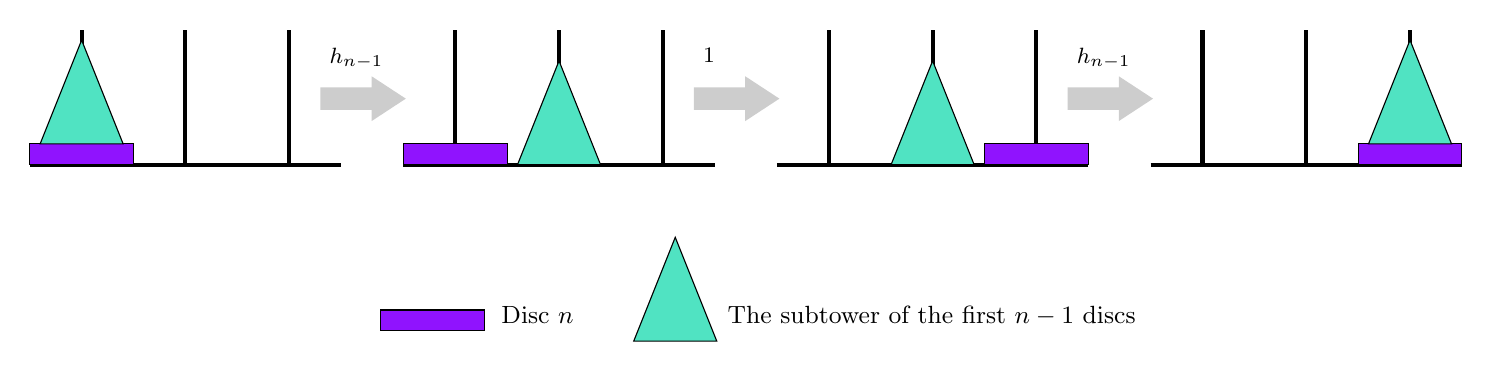
\begin{tikzpicture}[x=0.75pt,y=0.75pt,yscale=-1,xscale=1]
%uncomment if require: \path (0,241); %set diagram left start at 0, and has height of 241

%Straight Lines [id:da9282475701834738] 
\draw [line width=1.5]    (75,65) -- (75,0) ;
%Straight Lines [id:da8456727175187826] 
\draw [line width=1.5]    (125,65) -- (125,0) ;
%Straight Lines [id:da8245798231947901] 
\draw [line width=1.5]    (25,65) -- (25,0) ;
%Straight Lines [id:da31175258972263786] 
\draw [line width=1.5]    (0,65) -- (150,65) ;
%Shape: Rectangle [id:dp32704689003974163] 
\draw  [fill={rgb, 255:red, 144; green, 19; blue, 254 }  ,fill opacity=1 ] (0,55) -- (50,55) -- (50,65) -- (0,65) -- cycle ;
%Shape: Triangle [id:dp06889765992146213] 
\draw  [fill={rgb, 255:red, 80; green, 227; blue, 194 }  ,fill opacity=1 ] (25,5) -- (45,55) -- (5,55) -- cycle ;
%Straight Lines [id:da37562503022998284] 
\draw [line width=1.5]    (255,65) -- (255,0) ;
%Straight Lines [id:da46300649971101726] 
\draw [line width=1.5]    (305,65) -- (305,0) ;
%Straight Lines [id:da8693666197971948] 
\draw [line width=1.5]    (205,65) -- (205,0) ;
%Straight Lines [id:da3644645164104663] 
\draw [line width=1.5]    (180,65) -- (330,65) ;
%Shape: Rectangle [id:dp9483158274047903] 
\draw  [fill={rgb, 255:red, 144; green, 19; blue, 254 }  ,fill opacity=1 ] (180,55) -- (230,55) -- (230,65) -- (180,65) -- cycle ;
%Straight Lines [id:da21979758373938862] 
\draw [line width=1.5]    (435,65) -- (435,0) ;
%Straight Lines [id:da578932599170173] 
\draw [line width=1.5]    (485,65) -- (485,0) ;
%Straight Lines [id:da7050999519150514] 
\draw [line width=1.5]    (385,65) -- (385,0) ;
%Straight Lines [id:da4405911343620206] 
\draw [line width=1.5]    (360,65) -- (510,65) ;
%Shape: Rectangle [id:dp7574189708752779] 
\draw  [fill={rgb, 255:red, 144; green, 19; blue, 254 }  ,fill opacity=1 ] (460,55) -- (510,55) -- (510,65) -- (460,65) -- cycle ;
%Straight Lines [id:da47247880526508323] 
\draw [line width=1.5]    (615,65) -- (615,0) ;
%Straight Lines [id:da410691479483257] 
\draw [line width=1.5]    (665,65) -- (665,0) ;
%Straight Lines [id:da6499207875284638] 
\draw [line width=1.5]    (565,65) -- (565,0) ;
%Straight Lines [id:da18738816712523865] 
\draw [line width=1.5]    (540,65) -- (690,65) ;
%Shape: Rectangle [id:dp9401440468463176] 
\draw  [fill={rgb, 255:red, 144; green, 19; blue, 254 }  ,fill opacity=1 ] (640,55) -- (690,55) -- (690,65) -- (640,65) -- cycle ;
%Right Arrow [id:dp534613609568585] 
\draw  [draw opacity=0][fill={rgb, 255:red, 155; green, 155; blue, 155 }  ,fill opacity=0.5 ] (140,27.81) -- (164.71,27.81) -- (164.71,22.41) -- (181.18,33.2) -- (164.71,44) -- (164.71,38.6) -- (140,38.6) -- cycle ;
%Right Arrow [id:dp8712046365867925] 
\draw  [draw opacity=0][fill={rgb, 255:red, 155; green, 155; blue, 155 }  ,fill opacity=0.5 ] (320,27.81) -- (344.71,27.81) -- (344.71,22.41) -- (361.18,33.2) -- (344.71,44) -- (344.71,38.6) -- (320,38.6) -- cycle ;
%Right Arrow [id:dp1610359027602104] 
\draw  [draw opacity=0][fill={rgb, 255:red, 155; green, 155; blue, 155 }  ,fill opacity=0.5 ] (500,27.81) -- (524.71,27.81) -- (524.71,22.41) -- (541.18,33.2) -- (524.71,44) -- (524.71,38.6) -- (500,38.6) -- cycle ;
%Shape: Rectangle [id:dp8645342569013641] 
\draw  [fill={rgb, 255:red, 144; green, 19; blue, 254 }  ,fill opacity=1 ] (169,135) -- (219,135) -- (219,145) -- (169,145) -- cycle ;

%Shape: Triangle [id:dp547271885867356] 
\draw  [fill={rgb, 255:red, 80; green, 227; blue, 194 }  ,fill opacity=1 ] (311,100) -- (331,150) -- (291,150) -- cycle ;
%Shape: Triangle [id:dp6848694482352105] 
\draw  [fill={rgb, 255:red, 80; green, 227; blue, 194 }  ,fill opacity=1 ] (255,15) -- (275,65) -- (235,65) -- cycle ;
%Shape: Triangle [id:dp05180516619833431] 
\draw  [fill={rgb, 255:red, 80; green, 227; blue, 194 }  ,fill opacity=1 ] (435,15) -- (455,65) -- (415,65) -- cycle ;
%Shape: Triangle [id:dp8992062198078927] 
\draw  [fill={rgb, 255:red, 80; green, 227; blue, 194 }  ,fill opacity=1 ] (665,5) -- (685,55) -- (645,55) -- cycle ;

% Text Node
\draw (143.18,7.4) node [anchor=north west][inner sep=0.75pt]  [font=\footnotesize]  {$h_{n-1}$};
% Text Node
\draw (323.18,7.4) node [anchor=north west][inner sep=0.75pt]  [font=\footnotesize]  {$1$};
% Text Node
\draw (503.18,7.4) node [anchor=north west][inner sep=0.75pt]  [font=\footnotesize]  {$h_{n-1}$};
% Text Node
\draw (226,132) node [anchor=north west][inner sep=0.75pt]  [font=\small] [align=left] {Disc $\displaystyle n$};
% Text Node
\draw (335,132) node [anchor=north west][inner sep=0.75pt]  [font=\small] [align=left] {The subtower of the first $\displaystyle n-1$ discs};


\end{tikzpicture}
    \caption{An illustration of the recursive solution of the Tower of Hanoi }
    \label{fig:procedure}
\end{figure}

Several variations to the original Tower of Hanoi problem exist in the literature, such as forbidding certain moves
of discs between certain pegs \cite{atkinson1981cyclic,sapir2004tower,stockmeyer1994variations}, increasing the number
of pegs \cite{KLAVZAR2002141,stockmeyer1994variations} \cite[p. 25]{dudeney1958canterbury}, allowing discs to be placed on top of smaller discs \cite[Variant 1]{wood1980towers}, coloring discs \cite{stockmeyer2008new},
and  weighing the moves between pegs \cite{WTH}.  Some of these variants are still unsolved and continue to ignite research questions. However, simple variations can still lead to interesting recurrences. Composing these variants is for the sake of studying their combinatorial as well as algorithmic aspects. For more about the Tower of Hanoi
problem, we point the interested reader to the comprehensive monograph \cite{hinz2018tower}.







In this paper, we explore the richness of the Tower of Hanoi beyond its classical setting to explore the study of recurrences and proofs by induction, by introducing four new variants of the Tower of Hanoi, each has an optimal number of moves related to one of the four known numbers,  Fibonacci, Lucas, Jacobsthal, and Pell numbers. The goal behind designing these new variants is to:
\begin{itemize}
    \item Provide new combinatorial interpretations for  Fibonacci, Lucas, Jacobsthal, and Pell like numbers, using the framework of the Tower of Hanoi puzzle;
    \item These new variants can be used to introduce the concept of recursion in algorithms and sequences. Since the Tower of Hanoi problem and the Fibonacci sequence are the most common examples used to introduce the concept of recursion in algorithms and sequences, respectively.  Hence, these new variants provide a good example of how to introduce the concept of recursion for students since  they combine the Tower of Hanoi problem and the well-known Fibonacci, Lucas, Jacobsthal, and Pell recursive sequences. Therefore, these variants provide an excellent example to teach the mechanism of establishing recursive algorithms and recurrence relations.
    \item As it is shown in Section 3, these new variants produce four new recursive graph classes, that can be useful to expand the research in graph theory. 

\end{itemize}





Many classical sequences are related to the Tower of Hanoi puzzle and its variations. We mention here  Stern's diatomic sequence \cite{HINZ2005693}, the Stirling numbers of the second kind \cite{klavzarcombinatorics}, the second order Eulerian numbers,  Lah numbers and  Catalan numbers \cite{klavvzar2005hanoi},  the Anti-Ramsey numbers \cite{gorgol2019anti}, in addition to   Sierpinski gasket \cite{hinz1990average} and the Pascal triangle \cite{hinz1992pascal}.  Apart from the optimal solution, a link between the Tower of Hanoi and the Fibonacci sequence has been found in \cite{Discovering_fibonnaci}.

% \textcolor{red}{In particular, authors have shown that for $n$ discs, the number of key vertices in Hanoi graph $H_{3}^{n}$ is equal to the $(n-1)$th Fibonacci number, such that a vertex $v$ of $H_{3}^{}n$ is a key vertex if $d_{2}(v)=2d_{0}(v)$...
% of t is a station for which the minimum number of moves to transfer all discs to peg $3$ is exactly twice the minimum.}



% Let $U_{n}(p,q)$ denote the sequence defined recursively by
% \begin{equation}
%     U_{0}=0, U_{1}=1,\quad U_{n}=pU_{n-1}+qU_{n-2}, n\geq 2
% \end{equation}

% and let $V_{n}(p,q)$ be given by 

% \begin{equation}
%     V_{0}=2, V_{1}=p,\quad V_{n}=pV_{n-1}+qV_{n-2}, n\geq 2
% \end{equation}

% $U_{n}(p,q)$  and $V_{n}(p,q)$ are known as the  generalized Fibonacci and Lucas sequences, respectively \cite{generlized_fibo}.


We separate the main results of this paper into two main Sections. In Section 2, we present the four variants including their rules,  optimal solutions, and algorithms. Next, in Section 3, we present their associated graphs and establish some of their basic properties. We finish the paper with a conclusion, in addition to some remarks for further works and a proposition of a  possible generalization of the new four variants presented in this work. 



% {\color{red}Ideas : 

% \begin{itemize}

%     \item The tower of Hanoi is a typical components of any  introduction to algorithms
% or discrete mathematics.

% \item The tower of Hanoi is a familiar problem in many fields, as computer programming, algorithms, and discrete mathematics.

 


% \end{itemize}

% }



 

\section{The Towers of Fibonacci, Lucas, Jacobsthal, and Pell}

Along with the classical moves of the classical Tower of Hanoi that follow the rules $(r_{1})-(r_{3})$, here we introduce a new type of moves, called the Magic Moves. 

\begin{definition}
    Consider a Tower of Hanoi with $n\geq 2$ discs, and let $d$ be a disc such that $1<d\leq n$. When ignoring discs $d+1,\ldots,n$,  if disc $d$ is the topmost\footnote{A topmost disc of a peg is the disc on top of all the discs stacked onto that peg.} disc of its peg $i$, and disc $d-1$ is the bottommost\footnote{A bottommost disc of a peg is the disc in the bottom of all the discs stacked onto that peg.}  disc of its peg $k$, then discs $d$ and $d-1$ can be moved simultaneously using one move to peg $j\neq i,k$. This move is called a \textit{Magic move}.
\end{definition}
The magic move is considered as a bonus card that player can use to bend or break the classical rules of the Tower of Hanoi.  Figure \ref{fig:mag_move_exam} shows a case where the player can apply the magic move. The orange arrow in this and the following Figures corresponds to a use of a magic move.  

In the four variants presented in this work, we consider three pegs, $n$ discs, and the same objective. But the rules of plying are different from one variant to another. 

 
	\begin{figure}[H]
	    \centering
            

\tikzset{every picture/.style={line width=0.75pt}} %set default line width to 0.75pt        

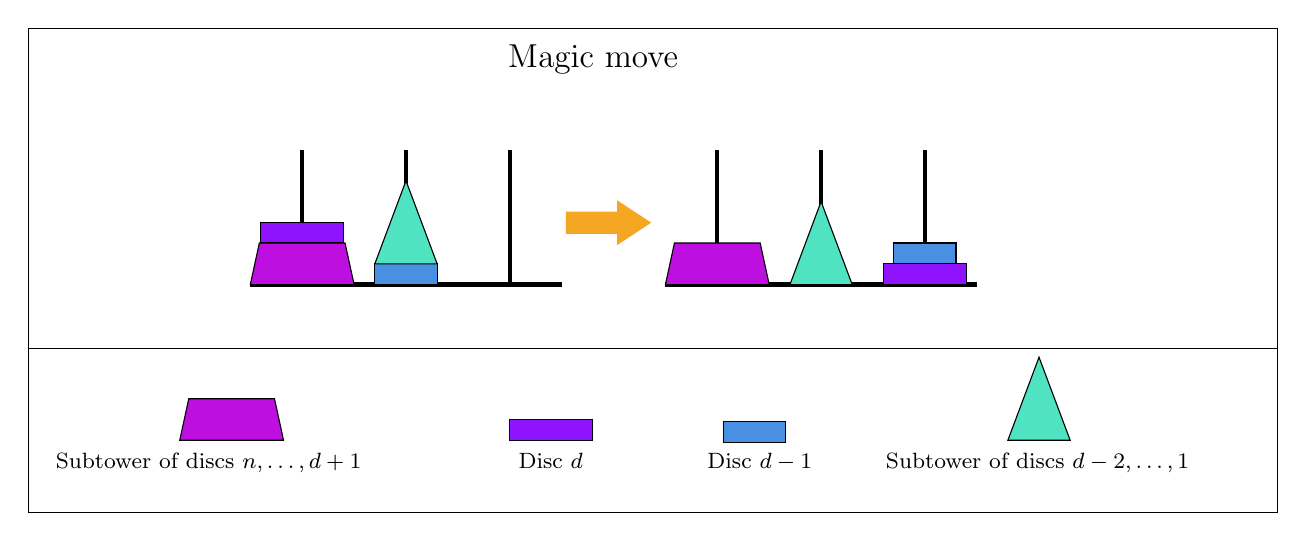
\begin{tikzpicture}[x=0.75pt,y=0.75pt,yscale=-1,xscale=1]
%uncomment if require: \path (0,365); %set diagram left start at 0, and has height of 365

%Straight Lines [id:da2433527856456119] 
\draw [line width=1.5]    (237,150) -- (237,85) ;
%Straight Lines [id:da12467546510005323] 
\draw [line width=1.5]    (287,150) -- (287,85) ;
%Straight Lines [id:da6661133221943116] 
\draw [line width=1.5]    (187,150) -- (187,85) ;
%Straight Lines [id:da876507202654921] 
\draw [line width=1.5]    (162,150) -- (312,150) ;
%Shape: Rectangle [id:dp9581710992755996] 
\draw  [fill={rgb, 255:red, 144; green, 19; blue, 254 }  ,fill opacity=1 ] (166.8,120) -- (206.8,120) -- (206.8,130) -- (166.8,130) -- cycle ;
%Shape: Rectangle [id:dp8402863453184108] 
\draw  [fill={rgb, 255:red, 74; green, 144; blue, 226 }  ,fill opacity=1 ] (222,140) -- (252,140) -- (252,150) -- (222,150) -- cycle ;
%Shape: Triangle [id:dp8282959416329734] 
\draw  [fill={rgb, 255:red, 80; green, 227; blue, 194 }  ,fill opacity=1 ] (237,100) -- (252,140) -- (222,140) -- cycle ;
%Shape: Trapezoid [id:dp17206160284989447] 
\draw  [fill={rgb, 255:red, 189; green, 16; blue, 224 }  ,fill opacity=1 ] (162,150) -- (166.35,130) -- (207.65,130) -- (212,150) -- cycle ;
%Straight Lines [id:da9363897255376088] 
\draw [line width=1.5]    (437,150) -- (437,85) ;
%Straight Lines [id:da5581881298896516] 
\draw [line width=1.5]    (487,150) -- (487,85) ;
%Straight Lines [id:da7500710046565593] 
\draw [line width=1.5]    (387,150) -- (387,85) ;
%Straight Lines [id:da03243354273668575] 
\draw [line width=1.5]    (362,150) -- (512,150) ;
%Shape: Rectangle [id:dp9137554325328925] 
\draw  [fill={rgb, 255:red, 144; green, 19; blue, 254 }  ,fill opacity=1 ] (467,140) -- (507,140) -- (507,150) -- (467,150) -- cycle ;
%Shape: Rectangle [id:dp8797795775448956] 
\draw  [fill={rgb, 255:red, 74; green, 144; blue, 226 }  ,fill opacity=1 ] (472,130) -- (502,130) -- (502,140) -- (472,140) -- cycle ;
%Shape: Triangle [id:dp4235756866358773] 
\draw  [fill={rgb, 255:red, 80; green, 227; blue, 194 }  ,fill opacity=1 ] (437,110) -- (452,150) -- (422,150) -- cycle ;
%Shape: Trapezoid [id:dp5348042276434657] 
\draw  [fill={rgb, 255:red, 189; green, 16; blue, 224 }  ,fill opacity=1 ] (362,150) -- (366.35,130) -- (407.65,130) -- (412,150) -- cycle ;
%Right Arrow [id:dp7411885527918458] 
\draw  [draw opacity=0][fill={rgb, 255:red, 245; green, 166; blue, 35 }  ,fill opacity=1 ] (314,114.81) -- (338.71,114.81) -- (338.71,109.41) -- (355.18,120.2) -- (338.71,131) -- (338.71,125.6) -- (314,125.6) -- cycle ;
%Shape: Trapezoid [id:dp5761586813750981] 
\draw  [fill={rgb, 255:red, 189; green, 16; blue, 224 }  ,fill opacity=1 ] (128,225) -- (132.35,205) -- (173.65,205) -- (178,225) -- cycle ;

%Shape: Rectangle [id:dp06928548817899349] 
\draw  [fill={rgb, 255:red, 144; green, 19; blue, 254 }  ,fill opacity=1 ] (287,215) -- (327,215) -- (327,225) -- (287,225) -- cycle ;

%Shape: Rectangle [id:dp9354576026846262] 
\draw  [fill={rgb, 255:red, 74; green, 144; blue, 226 }  ,fill opacity=1 ] (390,216) -- (420,216) -- (420,226) -- (390,226) -- cycle ;

%Shape: Triangle [id:dp5043879724591793] 
\draw  [fill={rgb, 255:red, 80; green, 227; blue, 194 }  ,fill opacity=1 ] (542,185) -- (557,225) -- (527,225) -- cycle ;

%Shape: Rectangle [id:dp8162339810622232] 
\draw   (55,26.5) -- (656.82,26.5) -- (656.82,259.95) -- (55,259.95) -- cycle ;
%Straight Lines [id:da9346086239123819] 
\draw    (55,180.95) -- (656.82,180.95) ;

% Text Node
\draw (285,33) node [anchor=north west][inner sep=0.75pt]  [font=\large] [align=left] {Magic move};
% Text Node
\draw (67,230) node [anchor=north west][inner sep=0.75pt]  [font=\footnotesize] [align=left] {Subtower of discs $\displaystyle n,\dotsc ,d+1$};
% Text Node
\draw (290,230) node [anchor=north west][inner sep=0.75pt]  [font=\footnotesize] [align=left] {Disc $\displaystyle d$};
% Text Node
\draw (381,230) node [anchor=north west][inner sep=0.75pt]  [font=\footnotesize] [align=left] {Disc $\displaystyle d-1$};
% Text Node
\draw (467,230) node [anchor=north west][inner sep=0.75pt]  [font=\footnotesize] [align=left] {Subtower of discs $\displaystyle d-2,\dotsc ,1$};


\end{tikzpicture}

	    \caption{An example of a    Magic move applied on disc $d>1$}
        \label{fig:mag_move_exam}
 	\end{figure}



In \cite[Section 6.1]{hinz2018tower},   Hinz et al. have defined a list of $5$ rules that each variant of the Tower of Hanoi problem should obey. Allowing the use of the Magic move violates the $4$th rule in the list of Hinz et al, namely, one or more discs can only be moved from the top of a stack, since that Magic move allows the move of two discs in the same time for which one of them does not need to be on the top of a stack. 

Next in this section, we present the new four variants of the Tower of Hanoi, each has its playing rules, for which the length of the resulting solution is related to one of the known numbers, Fibonacci, Lucas, Jacobsthal, or Pell, defined respectively by the following recurrence relations.  



\begin{equation}
    F_{0}=0,F_{1}=1,\quad F_{n}=F_{n-1}+F_{n-2}, n\geq2,
\end{equation}
\begin{equation}
    L_{0}=2, L_{1}=1,\quad  L_{n}= L_{n-1}+ L_{n-2}, n\geq2,
\end{equation}
\begin{equation}
    P_{0}=0,P_{1}=1,\quad P_{n}=2P_{n-1}+P_{n-2}, n\geq2,
\end{equation}
\begin{equation}
    J_{0}=0,J_{1}=1,\quad J_{n}=J_{n-1}+2J_{n-2}, n\geq2.
\end{equation}

 





\subsection{The Tower of Fibonacci}
% In this section, we present a new variant of the Tower of Hanoi, that we called Tower of Fibonacci. The minimum number of moves of this variant is related to Fibonacci numbers. 
In the Tower of Fibonacci, we consider the rules $(r_{1})-(r_{3})$, in addition to what we call, Fibonacci's rule $(f)$, which is defined as follows.
\begin{itemize}
    \item[$(f)$] The Magic move can be performed whenever its conditions are met.
\end{itemize}
% The solution to to this variant is related to Fibonacci numbers.


Let $\alpha_{n}$ be the minimum number of moves required to solve the Tower of  Fibonacci problem with $n\geq 0$ discs. Theorem \ref{theorem_fibona} provides a recurrence relation of  $\alpha_{n}$.

\begin{theorem}\label{theorem_fibona}
For all  $n\geq 2$, we have  
\begin{equation}
	\alpha_{n}=\alpha_{n-1}+\alpha_{n-2}+1,   
	\end{equation}
	where $\alpha_{0}=0$ and $\alpha_{1}=1$.
	\end{theorem}
    
    \begin{proof}
    We proceed by induction on $n$. For $n = 1$,  only one classical move is needed to transfer the unique disc from source peg to destination peg.
    
    Assume that the Tower of Fibonacci with $d<n$ discs can be solved optimally using $\alpha_{d}$ moves.  
    
    To solve a Tower of Fibonacci of $n$ discs, the largest disc $n$ needs to be liberated, i.e., no disc is above it. To proceed,  the first thing to do is to transfer the subtower of the first $n-1$ disc to the middle peg using $\alpha_{n-1}$ moves so that the largest disc can be moved directly to the destination peg, but when the subtower of the first $n-1$ is stacked onto the middle peg, and the largest disc is the only disc stacked onto the source peg,  the Magic move can be applied to move the largest disc and disc $n-1$ simultaneously and directly to the destination peg using only one move. By doing this, we obtain a state where the subtower of the first $n-2$ disc is stacked onto the middle peg, and discs $n$ and $n-1$ are stacked onto the destination peg, the subtower of the first $n-2$ disc can be then transferred to the destination peg using $\alpha_{n-2}$ moves and the problem will be solved using the minimum number of moves. An illustration of the used procedure in this proof can be found in Figure \ref{fig:Fibo}. The number of moves used in this procedure is $\alpha_{n-1}+1+\alpha_{n-2}$.
    
    Note that if the Magic move was not used to transfer the largest disc $n$ and disc $n-1$ simultaneously, the final number of moves will be necessarily bigger than $\alpha_{n-1}+1+\alpha_{n-2}$, which is clearly not optimal. 

    \end{proof}
Using the proof of Theorem \ref{theorem_fibona}, we can design the Algorithm \ref{Alg:Fibonacci} that can be used to solve the Tower of Fibonacci problem. 


\begin{corollary}
    Algorithm \ref{Alg:Fibonacci} provides an optimal solution to the Tower of Fibonacci problem.
\end{corollary}
\begin{proof}
    It can be deduced from the proof of Theorem \ref{theorem_fibona}. 
\end{proof}


\begin{algorithm}[H]
\caption{Solution of the Tower of Fibonacci}
\label{Alg:Fibonacci}
\begin{algorithmic}[1]
\Procedure{Fibonacci}{$n,i,j$}
\State $k:=6-i-j;$
\If{$n=1$}
\State move disc $1$ from peg $i$ to peg $j$;
\Else
\State \textsc{Fibonacci}($n-1,i,k$);
\State move discs $n$ and $n-1$ simultaneously  to peg $j$ using Magic move;
\State \textsc{Fibonacci}($n-2,k,j$);
\EndIf
\EndProcedure
\end{algorithmic}
\end{algorithm}
The relation between the solution of the Tower Fibonacci   and the Fibonacci numbers is given in Corollary \ref{coro:fibonacci} and it can be proven easily using induction. The first values of $\alpha_{n}$ and the corresponding Fibonacci numbers are given in Table \ref{tab:fibonacci}.
    \begin{corollary}\label{coro:fibonacci}
        For all  $n\geq 2$, we have 
        \begin{equation}
            \alpha_{n}= F_{n+2}-1.
        \end{equation}
    \end{corollary}

    
\begin{table}[H]
\centering
\begin{tabular}{@{}lllllllllll@{}}
\toprule
$n$       & 0 & 1 & 2 & 3 & 4 & 5  & 6  & 7  & 8  & $\cdots$ \\ \midrule
$\alpha_{n}$   & 0 & 1 & 2 & 4 & 7 & 12 & 20 & 33 & 54 & $\cdots$ \\
$F_{n+2}$ & 1 & 2 & 3 & 5 & 8 & 13 & 21 & 34 & 55 & $\cdots$ \\ \bottomrule
\end{tabular}
\caption{First values of $\alpha_{n}$ and $F_{n+2}$ }
\label{tab:fibonacci}
\end{table}
As a direct result of Corollary \ref{coro:fibonacci},  the number of states in the optimal sequence of moves of the Tower of Fibonacci is exactly $F_{n+2}$.







Giving that $F_{n}=\dfrac{\varphi^{n}-\psi^{n}}{\sqrt{5}}$, where $\varphi^{n}=\dfrac{1+\sqrt{5}}{2}$ is the golden ratio, and $\psi^{n}=\dfrac{1-\sqrt{5}}{2}$ is its conjugate. Then, a closed formula for $\alpha_{n}$ can be deduced. 
\begin{corollary}
    For all $n\geq 0$, we have 
    \begin{equation}
        \alpha_{n}=\dfrac{\varphi^{n+2}-\psi^{n+2}}{\sqrt{5}}-1
    \end{equation}
\end{corollary}


    
    
	% \begin{theorem}
	% The linear tower of Fibonacci of $n$ discs can be solved optimally using the following number of moves
	% \begin{equation}
	%     v_{n}=v_{n-1}+2v_{n-2}+3
	% \end{equation}
	%  with $v_{0}=0,$ $v_{1}=2,$ $v_{2}=5$.
	% \end{theorem}
	% We can see that $v_{n}$ is a kind of Jacobsthal sequence.


Figure \ref{fig:Fibo}   illustrates the process of Fibonacci's Tower solution, where the numbers above the arrows are the number of moves required to reach the next state in the Figure.
\begin{figure}[H]
    \centering
    

\tikzset{every picture/.style={line width=0.75pt}} %set default line width to 0.75pt        

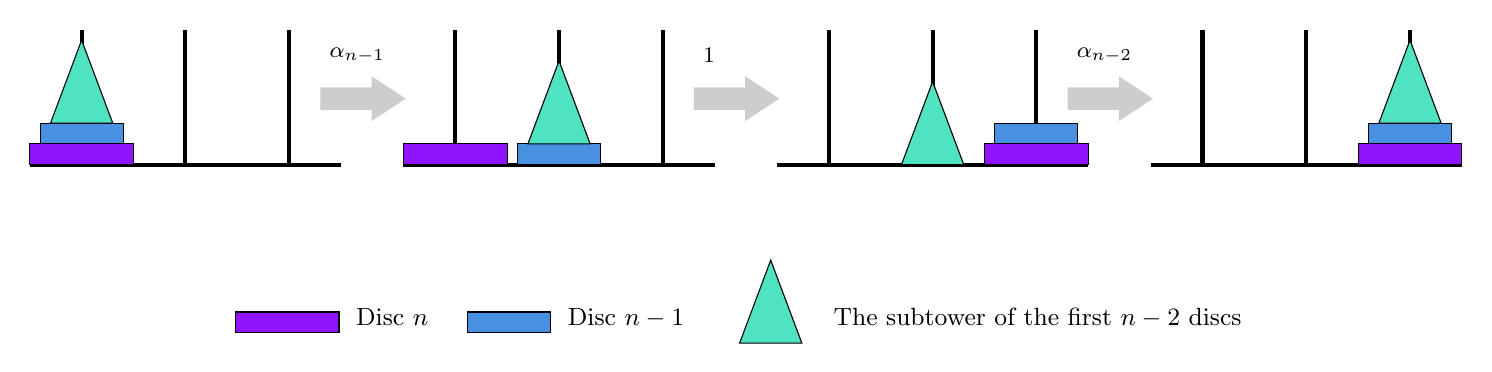
\begin{tikzpicture}[x=0.75pt,y=0.75pt,yscale=-1,xscale=1]
%uncomment if require: \path (0,241); %set diagram left start at 0, and has height of 241

%Straight Lines [id:da24815424100458983] 
\draw [line width=1.5]    (75,65) -- (75,0) ;
%Straight Lines [id:da8115465333076248] 
\draw [line width=1.5]    (125,65) -- (125,0) ;
%Straight Lines [id:da9739766763946329] 
\draw [line width=1.5]    (25,65) -- (25,0) ;
%Straight Lines [id:da6210476839521044] 
\draw [line width=1.5]    (0,65) -- (150,65) ;
%Shape: Rectangle [id:dp9225038130009493] 
\draw  [fill={rgb, 255:red, 74; green, 144; blue, 226 }  ,fill opacity=1 ] (5,45) -- (45,45) -- (45,55) -- (5,55) -- cycle ;
%Shape: Rectangle [id:dp9657809601082321] 
\draw  [fill={rgb, 255:red, 144; green, 19; blue, 254 }  ,fill opacity=1 ] (0,55) -- (50,55) -- (50,65) -- (0,65) -- cycle ;
%Shape: Triangle [id:dp7994638232866984] 
\draw  [fill={rgb, 255:red, 80; green, 227; blue, 194 }  ,fill opacity=1 ] (25,5) -- (40,45) -- (10,45) -- cycle ;
%Straight Lines [id:da6351702401045551] 
\draw [line width=1.5]    (255,65) -- (255,0) ;
%Straight Lines [id:da23539284354694123] 
\draw [line width=1.5]    (305,65) -- (305,0) ;
%Straight Lines [id:da6407367265186239] 
\draw [line width=1.5]    (205,65) -- (205,0) ;
%Straight Lines [id:da8823485940887543] 
\draw [line width=1.5]    (180,65) -- (330,65) ;
%Shape: Rectangle [id:dp7145285546098397] 
\draw  [fill={rgb, 255:red, 74; green, 144; blue, 226 }  ,fill opacity=1 ] (235,55) -- (275,55) -- (275,65) -- (235,65) -- cycle ;
%Shape: Rectangle [id:dp11686590820323883] 
\draw  [fill={rgb, 255:red, 144; green, 19; blue, 254 }  ,fill opacity=1 ] (180,55) -- (230,55) -- (230,65) -- (180,65) -- cycle ;
%Shape: Triangle [id:dp326144810998521] 
\draw  [fill={rgb, 255:red, 80; green, 227; blue, 194 }  ,fill opacity=1 ] (255,15) -- (270,55) -- (240,55) -- cycle ;
%Straight Lines [id:da38727899106831454] 
\draw [line width=1.5]    (435,65) -- (435,0) ;
%Straight Lines [id:da4098652212962761] 
\draw [line width=1.5]    (485,65) -- (485,0) ;
%Straight Lines [id:da6850068143481041] 
\draw [line width=1.5]    (385,65) -- (385,0) ;
%Straight Lines [id:da8948080700978496] 
\draw [line width=1.5]    (360,65) -- (510,65) ;
%Shape: Rectangle [id:dp7946080570799627] 
\draw  [fill={rgb, 255:red, 74; green, 144; blue, 226 }  ,fill opacity=1 ] (465,45) -- (505,45) -- (505,55) -- (465,55) -- cycle ;
%Shape: Rectangle [id:dp5580963644428822] 
\draw  [fill={rgb, 255:red, 144; green, 19; blue, 254 }  ,fill opacity=1 ] (460,55) -- (510,55) -- (510,65) -- (460,65) -- cycle ;
%Shape: Triangle [id:dp20454638540295167] 
\draw  [fill={rgb, 255:red, 80; green, 227; blue, 194 }  ,fill opacity=1 ] (435,25) -- (450,65) -- (420,65) -- cycle ;
%Straight Lines [id:da71545551051053] 
\draw [line width=1.5]    (615,65) -- (615,0) ;
%Straight Lines [id:da42952519976526493] 
\draw [line width=1.5]    (665,65) -- (665,0) ;
%Straight Lines [id:da02676389926063205] 
\draw [line width=1.5]    (565,65) -- (565,0) ;
%Straight Lines [id:da513368833927792] 
\draw [line width=1.5]    (540,65) -- (690,65) ;
%Shape: Rectangle [id:dp9163905899859819] 
\draw  [fill={rgb, 255:red, 74; green, 144; blue, 226 }  ,fill opacity=1 ] (645,45) -- (685,45) -- (685,55) -- (645,55) -- cycle ;
%Shape: Rectangle [id:dp23350695623157525] 
\draw  [fill={rgb, 255:red, 144; green, 19; blue, 254 }  ,fill opacity=1 ] (640,55) -- (690,55) -- (690,65) -- (640,65) -- cycle ;
%Shape: Triangle [id:dp5086883694866662] 
\draw  [fill={rgb, 255:red, 80; green, 227; blue, 194 }  ,fill opacity=1 ] (665,5) -- (680,45) -- (650,45) -- cycle ;
%Right Arrow [id:dp02688709887459506] 
\draw  [draw opacity=0][fill={rgb, 255:red, 155; green, 155; blue, 155 }  ,fill opacity=0.5 ] (140,27.81) -- (164.71,27.81) -- (164.71,22.41) -- (181.18,33.2) -- (164.71,44) -- (164.71,38.6) -- (140,38.6) -- cycle ;
%Right Arrow [id:dp7559893443766514] 
\draw  [draw opacity=0][fill={rgb, 255:red, 155; green, 155; blue, 155 }  ,fill opacity=0.5 ] (320,27.81) -- (344.71,27.81) -- (344.71,22.41) -- (361.18,33.2) -- (344.71,44) -- (344.71,38.6) -- (320,38.6) -- cycle ;
%Right Arrow [id:dp6938789629236952] 
\draw  [draw opacity=0][fill={rgb, 255:red, 155; green, 155; blue, 155 }  ,fill opacity=0.5 ] (500,27.81) -- (524.71,27.81) -- (524.71,22.41) -- (541.18,33.2) -- (524.71,44) -- (524.71,38.6) -- (500,38.6) -- cycle ;
%Shape: Rectangle [id:dp8166502832119333] 
\draw  [fill={rgb, 255:red, 144; green, 19; blue, 254 }  ,fill opacity=1 ] (99,136) -- (149,136) -- (149,146) -- (99,146) -- cycle ;

%Shape: Rectangle [id:dp6910609554250948] 
\draw  [fill={rgb, 255:red, 74; green, 144; blue, 226 }  ,fill opacity=1 ] (211,136) -- (251,136) -- (251,146) -- (211,146) -- cycle ;

%Shape: Triangle [id:dp018656944685809806] 
\draw  [fill={rgb, 255:red, 80; green, 227; blue, 194 }  ,fill opacity=1 ] (357,111) -- (372,151) -- (342,151) -- cycle ;


% Text Node
\draw (143.18,7.4) node [anchor=north west][inner sep=0.75pt]  [font=\footnotesize]  {$\alpha_{n-1}$};
% Text Node
\draw (323.18,7.4) node [anchor=north west][inner sep=0.75pt]  [font=\footnotesize]  {$1$};
% Text Node
\draw (503.18,7.4) node [anchor=north west][inner sep=0.75pt]  [font=\footnotesize]  {$\alpha_{n-2}$};
% Text Node
\draw (258,133) node [anchor=north west][inner sep=0.75pt]  [font=\small] [align=left] {Disc $\displaystyle n-1$};
% Text Node
\draw (156,133) node [anchor=north west][inner sep=0.75pt]  [font=\small] [align=left] {Disc $\displaystyle n$};
% Text Node
\draw (386,133) node [anchor=north west][inner sep=0.75pt]  [font=\small] [align=left] {The subtower of the first $\displaystyle n-2$ discs};


\end{tikzpicture}
    \caption{Illustration of the solution of Fibonacci's Tower for $n\geq 2$}
    \label{fig:Fibo}
\end{figure}

The Tower of Fibonacci variant is not the first Tower of Hanoi variant with an optimal solution related to Fibonacci numbers.   Mneimneh in \cite[Section 7]{simple_var} presented the Beam Me Up Scotty problem which is a variant of the Tower of Hanoi, for which disc $i$ for $1 < i < n$ is moved for free between the two disks $i - 1$ and $i + 1$,
whenever the former is sitting directly on top of the latter. Rittaud if \cite{rittaud2022fibonacci} presented another variant of the Tower of Hanoi, in this variant, only $k-$Fibonacci moves are allowed. A $k-$Fibonacci move as it is defined in   \cite{rittaud2022fibonacci} seems to be identical to the Magic move but with a different interpretation. In contrast to Rittaud's variant for which only $k-$Fibonacci moves are allowed,  the Tower of Fibonacci variant allows the classical moves as well as the Magic move.

 

\begin{proposition}
    The only states where no Magic move can be applied are the perfect states\footnote{A perfect state is a state where all discs are stacked onto one single peg.}.
\end{proposition}
\begin{proof}
The Magic move can not be used for disc $1$ since it is the smallest disc, so for any state where disc $1$ is the only topmost disc, the Magic move is no longer useful. The states where the only topmost disc that exists is the smallest are the perfect states. 
\end{proof}






 
\subsection{The tower of Lucas}
In the Tower of Lucas problem, we consider the rules $(r_{1})-(r_{3})$, $(f)$, in addition to Lucas's rule $(l)$ described below.
\begin{itemize}
    \item[$(l)$] The smallest disc $1$, takes always two moves to reach its destination. 
\end{itemize}

In other words, Lucas's rule $(l)$ means that the smallest disc always takes the longest path to reach its destination, which implies that if disc $1$ is to be moved from peg $i$ to peg $j$, it must first go through peg $k$. 

The solution to this variant will relate the optimal number of moves in a Tower of Hanoi problem to the Lucas numbers.

Let $\beta_{n}$ be the minimum number of moves required to solve the Tower of  Lucas problem with $n\geq 0$ discs. A recurrence relation of this number is given in the next Theorem.  
    \begin{theorem}
    For all $n\geq 2$, we have
    \begin{equation}
        \beta_{n}=\beta_{n-1}+\beta_{n-2}+1
    \end{equation}
    where $\beta_{0}=0$ and $\beta_{1}=2$.
    \end{theorem}   
    \begin{proof}
    The procedure to solve the Tower of Lucas with $n$ discs is the same as the one used to solve the Tower of Fibonacci that was described in the proof of Theorem \ref{theorem_fibona}, except the case where $n=1$, in which the smallest disc $1$ takes two moves to be transferred from source peg to destination peg, which implies that $\beta_{1}=2$.
    \end{proof}

The relation between the solution of the Tower Lucas  and the Lucas numbers is given in Corollary \ref{coro:lucas} and it can be proven easily using induction. The first values of $\beta_{n}$ and the corresponding Lucas numbers are given in Table \ref{tab:lucas}.
    
    \begin{corollary}\label{coro:lucas}
        For all $n\geq 0$, we have 
        \begin{equation}
            \beta_{n}=L_{n+1}-1.
        \end{equation}
    \end{corollary}
\begin{table}[H]
\centering
\begin{tabular}{@{}lllllllllll@{}}
\toprule
$n$       & 0 & 1 & 2 & 3 & 4  & 5  & 6  & 7  & 8  & $\cdots$ \\ \midrule
$\beta_{n}$   & 0 & 2 & 3 & 6 & 10 & 17 & 28 & 46 & 75 & $\cdots$ \\
$L_{n+1}$ & 1 & 3 & 4 & 7 & 11 & 18 & 29 & 47 & 76 & $\cdots$ \\ \bottomrule
\end{tabular}
\caption{First values of $\beta_{n}$ and $L_{n+1}$ }\label{tab:lucas}
\end{table}

Giving that $L_{n}=\varphi^{n}+\psi^{n}$. Then, a closed formula for $\beta_{n}$ can be deduced. 

\begin{corollary}
    For all $n\geq 0$, we have
    \begin{equation}
        \beta_{n}=\varphi^{n+1}+\psi^{n+1}-1
    \end{equation}
\end{corollary}

\begin{algorithm}[H]
\caption{Solution of the Tower of Lucas}
\label{Alg:Lucas}
\begin{algorithmic}[1]
\Procedure{Lucas}{$n,i,j$}
\State $k:=6-i-j;$
\If{$n=1$}
\State move disc $1$ from peg $i$ to peg $k$;
\State move disc $1$ from peg $k$ to peg $j$;

\Else
\State \textsc{Lucas}($n-1,i,k$);
\State move discs $n$ and $n-1$ simultaneously  to peg $j$ using Magic move;
\State \textsc{Lucas}($n-2,k,j$);
\EndIf
\EndProcedure
\end{algorithmic}
\end{algorithm}




    \subsection{The tower of Jacobsthal}

In the linear Tower of Hanoi \cite[Section 8.3.5]{hinz2018tower}, moves between the source peg $1$ and the destination peg $3$ are not allowed, hence, a disc can be moved only to an adjacent peg. This variant has been addressed first
in \cite[Section 3]{stockmeyer1994variations} and studied intensely in literature.  In the Tower of Jacobsthal variant, we consider the rules $(r_{1})-(r_{3}),(f)$, in addition the the Jacobsthal rules $(j_{1})$ and $(j_{2})$ described below.
\begin{itemize}
    \item[$(j_{1})$] A disc $d>1$ can not be moved directly between pegs $1$ and $3$.
    \item[$(j_{2})$] The magic move can not be used to transfer disc $d>1$ and $d-1$ simultaneously if disc $d$ is stacked onto peg $2$ and disc $d-1$ is stacked onto peg $3$.
\end{itemize}

As we can see, the only allowed moves in the  Tower of Jacobsthal are those between adjacent pegs for any disc $d>1$, as is the case in the linear Tower of Hanoi. 

The solution to this variant will relate the optimal number of moves in a Tower of Hanoi problem to the Jacobsthal numbers.



Let $\gamma_{n}$ be the minimum number of moves required to solve the Tower of  Jacobsthal problem with $n\geq 0$ discs. The next Theorem gives a recurrence relation of $\gamma_{n}$, in addition to a procedure to solve the Tower of  Jacobsthal problem described in the proof.
    \begin{theorem}
    For all $n\geq 2$, we have
    \begin{equation}
        \gamma_{n}=\gamma_{n-1}+2\gamma_{n-2}+3.
    \end{equation}
    with $\gamma_{0}=0$, $\gamma_{1}=1$.
    \end{theorem}
    \begin{proof}
     We proceed by induction on $n$. For the case, $n = 1$, disc $1$ can be moved directly from the source peg to the destination peg since it is not concerned by the rule of Jacobsthal.   Now, let us assume that the Tower of Jacobsthal with $k<n$ discs can be solved optimally using $\gamma_{k}$ moves.  
    
    Since disc $n>1$ cannot be moved directly to the destination peg due to Jacobsthal's rule, the first step in solving a Tower of Jacobsthal with  $n>1$ discs is to liberate the largest disc $n$, ensuring that the middle peg is empty. To proceed, the subtower of the first $n-1$ disc should be transferred to the destination peg using $\gamma_{n-1}$ moves so that the largest disc $n$ with disc $n-1$ can be moved to the middle peg simultaneously with disc $n-1$ using one single move, namely the Magic move. Then disc $n-1$ is moved to source peg using one move, so that disc $n$ will be free to move; note that this move can not be a Magic move according to Jacobsthal rule $(j_{2})$, because disc $n-1$ is stacked onto peg $2$ and disc $n-2$ is stacked onto peg $3$. The subtower of the first $n-2$ discs should be moved to the source peg using $\gamma_{n-2}$ to clear the destination peg, and then discs $n$ and $n-1$ can be moved directly to the destination peg using only one move, namely Magic move.  Finally, the sub-tower of the first $n-2$ disc is moved  to the destination peg using $\gamma_{n-2}$ moves. 

    
    An illustration of the used procedure in this proof can be found in Figure \ref{fig:Jaco}. The number of moves used in this procedure is $\gamma_{n-1}+1+1+\gamma_{n-2}+1+\gamma_{n-2}$. Hence, the result.
    \end{proof}

\begin{corollary}\label{coro:jacob}
    For all $n\geq 0$, we have 
    \begin{equation}
        \gamma_{n}=J_{n+2}-1-\frac{1}{2}(1-(-1)^{n}).
    \end{equation}
\end{corollary}

The relation between the solution of the Tower Jacobsthal  and the Jacobsthal numbers is given in Corollary \ref{coro:jacob} and it can be proven easily using induction. The first values of $\gamma_{n}$ and the corresponding Jacobsthal numbers are given in Table \ref{tab:jacob}.


\begin{table}[H]
\centering
\begin{tabular}{@{}lllllllllll@{}}
\toprule
$n$       & 0 & 1 & 2 & 3  & 4  & 5  & 6  & 7   & 8   & $\cdots$ \\ \midrule
$\gamma_{n}$   & 0 & 1 & 4 & 9  & 20 & 41 & 84 & 169 & 340 & $\cdots$ \\
$J_{n+2}$ & 1 & 3 & 5 & 11 & 21 & 43 & 85 & 171 & 341 & $\cdots$ \\ \bottomrule
\end{tabular}
\caption{First values of $\gamma_{n}$ and $J_{n+2}$ }\label{tab:jacob}
\end{table}


\begin{figure}[H]
    \centering
    

\tikzset{every picture/.style={line width=0.75pt}} %set default line width to 0.75pt        

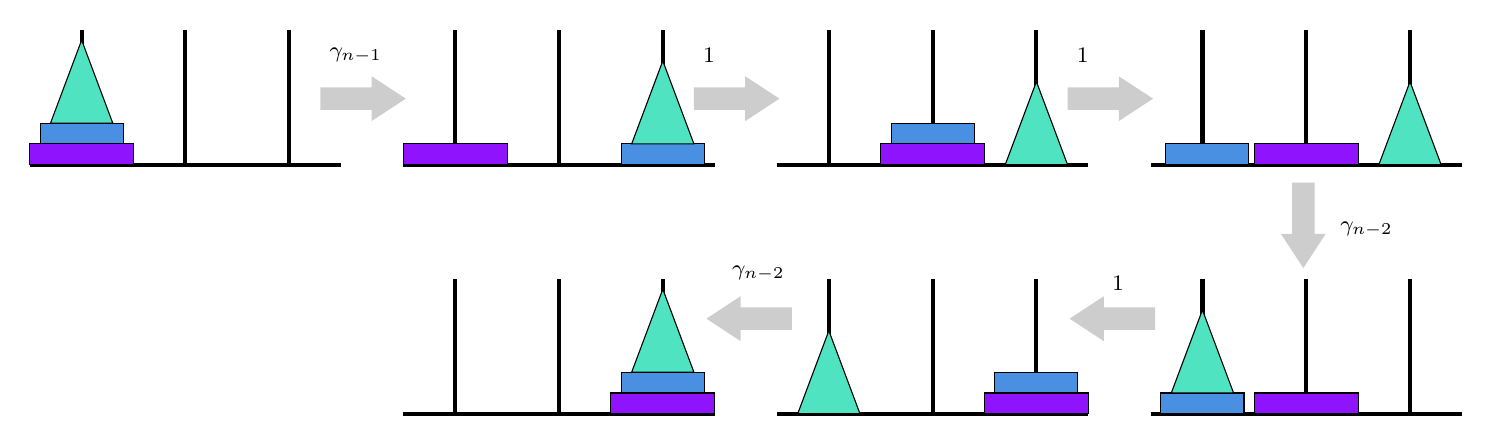
\begin{tikzpicture}[x=0.75pt,y=0.75pt,yscale=-1,xscale=1]
%uncomment if require: \path (0,261); %set diagram left start at 0, and has height of 261

%Straight Lines [id:da09074090299895055] 
\draw [line width=1.5]    (75,65) -- (75,0) ;
%Straight Lines [id:da4638154794848921] 
\draw [line width=1.5]    (125,65) -- (125,0) ;
%Straight Lines [id:da2875364013554764] 
\draw [line width=1.5]    (25,65) -- (25,0) ;
%Straight Lines [id:da24059486514465545] 
\draw [line width=1.5]    (0,65) -- (150,65) ;
%Shape: Rectangle [id:dp670448407383275] 
\draw  [fill={rgb, 255:red, 74; green, 144; blue, 226 }  ,fill opacity=1 ] (5,45) -- (45,45) -- (45,55) -- (5,55) -- cycle ;
%Shape: Rectangle [id:dp6358928927157512] 
\draw  [fill={rgb, 255:red, 144; green, 19; blue, 254 }  ,fill opacity=1 ] (0,55) -- (50,55) -- (50,65) -- (0,65) -- cycle ;
%Shape: Triangle [id:dp3701576402704907] 
\draw  [fill={rgb, 255:red, 80; green, 227; blue, 194 }  ,fill opacity=1 ] (25,5) -- (40,45) -- (10,45) -- cycle ;
%Straight Lines [id:da9365320297868673] 
\draw [line width=1.5]    (255,65) -- (255,0) ;
%Straight Lines [id:da38264248565012027] 
\draw [line width=1.5]    (305,65) -- (305,0) ;
%Straight Lines [id:da2753360012000532] 
\draw [line width=1.5]    (205,65) -- (205,0) ;
%Straight Lines [id:da7228701852848676] 
\draw [line width=1.5]    (180,65) -- (330,65) ;
%Shape: Rectangle [id:dp5529422103419381] 
\draw  [fill={rgb, 255:red, 74; green, 144; blue, 226 }  ,fill opacity=1 ] (285,55) -- (325,55) -- (325,65) -- (285,65) -- cycle ;
%Shape: Rectangle [id:dp8066781731357955] 
\draw  [fill={rgb, 255:red, 144; green, 19; blue, 254 }  ,fill opacity=1 ] (180,55) -- (230,55) -- (230,65) -- (180,65) -- cycle ;
%Shape: Triangle [id:dp19155257289523497] 
\draw  [fill={rgb, 255:red, 80; green, 227; blue, 194 }  ,fill opacity=1 ] (305,15) -- (320,55) -- (290,55) -- cycle ;
%Straight Lines [id:da7912931689528242] 
\draw [line width=1.5]    (435,65) -- (435,0) ;
%Straight Lines [id:da07171546376806237] 
\draw [line width=1.5]    (485,65) -- (485,0) ;
%Straight Lines [id:da12415907113119085] 
\draw [line width=1.5]    (385,65) -- (385,0) ;
%Straight Lines [id:da4740415163284728] 
\draw [line width=1.5]    (360,65) -- (510,65) ;
%Shape: Rectangle [id:dp9993190286937121] 
\draw  [fill={rgb, 255:red, 74; green, 144; blue, 226 }  ,fill opacity=1 ] (415,45) -- (455,45) -- (455,55) -- (415,55) -- cycle ;
%Shape: Rectangle [id:dp5947272920927318] 
\draw  [fill={rgb, 255:red, 144; green, 19; blue, 254 }  ,fill opacity=1 ] (410,55) -- (460,55) -- (460,65) -- (410,65) -- cycle ;
%Shape: Triangle [id:dp053982188115058616] 
\draw  [fill={rgb, 255:red, 80; green, 227; blue, 194 }  ,fill opacity=1 ] (485,25) -- (500,65) -- (470,65) -- cycle ;
%Straight Lines [id:da9103860243313793] 
\draw [line width=1.5]    (615,65) -- (615,0) ;
%Straight Lines [id:da32858546858295123] 
\draw [line width=1.5]    (665,65) -- (665,0) ;
%Straight Lines [id:da6579685310750645] 
\draw [line width=1.5]    (565,65) -- (565,0) ;
%Straight Lines [id:da5400882317586289] 
\draw [line width=1.5]    (540,65) -- (690,65) ;
%Shape: Rectangle [id:dp6301044837983836] 
\draw  [fill={rgb, 255:red, 74; green, 144; blue, 226 }  ,fill opacity=1 ] (547,55) -- (587,55) -- (587,65) -- (547,65) -- cycle ;
%Shape: Rectangle [id:dp3641042067761522] 
\draw  [fill={rgb, 255:red, 144; green, 19; blue, 254 }  ,fill opacity=1 ] (590,55) -- (640,55) -- (640,65) -- (590,65) -- cycle ;
%Shape: Triangle [id:dp9502837985538493] 
\draw  [fill={rgb, 255:red, 80; green, 227; blue, 194 }  ,fill opacity=1 ] (665,25) -- (680,65) -- (650,65) -- cycle ;
%Right Arrow [id:dp37639806414246446] 
\draw  [draw opacity=0][fill={rgb, 255:red, 155; green, 155; blue, 155 }  ,fill opacity=0.5 ] (140,27.81) -- (164.71,27.81) -- (164.71,22.41) -- (181.18,33.2) -- (164.71,44) -- (164.71,38.6) -- (140,38.6) -- cycle ;
%Right Arrow [id:dp20896573661751305] 
\draw  [draw opacity=0][fill={rgb, 255:red, 155; green, 155; blue, 155 }  ,fill opacity=0.5 ] (320,27.81) -- (344.71,27.81) -- (344.71,22.41) -- (361.18,33.2) -- (344.71,44) -- (344.71,38.6) -- (320,38.6) -- cycle ;
%Right Arrow [id:dp43926848719743816] 
\draw  [draw opacity=0][fill={rgb, 255:red, 155; green, 155; blue, 155 }  ,fill opacity=0.5 ] (500,27.81) -- (524.71,27.81) -- (524.71,22.41) -- (541.18,33.2) -- (524.71,44) -- (524.71,38.6) -- (500,38.6) -- cycle ;
%Straight Lines [id:da26709829663339346] 
\draw [line width=1.5]    (615,185) -- (615,120) ;
%Straight Lines [id:da07826776747136632] 
\draw [line width=1.5]    (665,185) -- (665,120) ;
%Straight Lines [id:da45605863847911055] 
\draw [line width=1.5]    (565,185) -- (565,120) ;
%Straight Lines [id:da3634980012559299] 
\draw [line width=1.5]    (540,185) -- (690,185) ;
%Shape: Rectangle [id:dp6692307603604473] 
\draw  [fill={rgb, 255:red, 74; green, 144; blue, 226 }  ,fill opacity=1 ] (545,175) -- (585,175) -- (585,185) -- (545,185) -- cycle ;
%Shape: Rectangle [id:dp5018382622593163] 
\draw  [fill={rgb, 255:red, 144; green, 19; blue, 254 }  ,fill opacity=1 ] (590,175) -- (640,175) -- (640,185) -- (590,185) -- cycle ;
%Shape: Triangle [id:dp6381352583231126] 
\draw  [fill={rgb, 255:red, 80; green, 227; blue, 194 }  ,fill opacity=1 ] (565,135) -- (580,175) -- (550,175) -- cycle ;
%Straight Lines [id:da8070688829137709] 
\draw [line width=1.5]    (435,185) -- (435,120) ;
%Straight Lines [id:da3413207916541259] 
\draw [line width=1.5]    (485,185) -- (485,120) ;
%Straight Lines [id:da22834213242494128] 
\draw [line width=1.5]    (385,185) -- (385,120) ;
%Straight Lines [id:da02400701269114114] 
\draw [line width=1.5]    (360,185) -- (510,185) ;
%Shape: Rectangle [id:dp9255763071768974] 
\draw  [fill={rgb, 255:red, 74; green, 144; blue, 226 }  ,fill opacity=1 ] (465,165) -- (505,165) -- (505,175) -- (465,175) -- cycle ;
%Shape: Rectangle [id:dp8115477734648835] 
\draw  [fill={rgb, 255:red, 144; green, 19; blue, 254 }  ,fill opacity=1 ] (460,175) -- (510,175) -- (510,185) -- (460,185) -- cycle ;
%Shape: Triangle [id:dp6233659669086451] 
\draw  [fill={rgb, 255:red, 80; green, 227; blue, 194 }  ,fill opacity=1 ] (385,145) -- (400,185) -- (370,185) -- cycle ;
%Straight Lines [id:da5140345148370122] 
\draw [line width=1.5]    (255,185) -- (255,120) ;
%Straight Lines [id:da45579214315375793] 
\draw [line width=1.5]    (305,185) -- (305,120) ;
%Straight Lines [id:da18294487610555943] 
\draw [line width=1.5]    (205,185) -- (205,120) ;
%Straight Lines [id:da7173511897559335] 
\draw [line width=1.5]    (180,185) -- (330,185) ;
%Shape: Rectangle [id:dp7533809364194062] 
\draw  [fill={rgb, 255:red, 74; green, 144; blue, 226 }  ,fill opacity=1 ] (285,165) -- (325,165) -- (325,175) -- (285,175) -- cycle ;
%Shape: Rectangle [id:dp740803336194769] 
\draw  [fill={rgb, 255:red, 144; green, 19; blue, 254 }  ,fill opacity=1 ] (280,175) -- (330,175) -- (330,185) -- (280,185) -- cycle ;
%Shape: Triangle [id:dp11826555581913167] 
\draw  [fill={rgb, 255:red, 80; green, 227; blue, 194 }  ,fill opacity=1 ] (305,125) -- (320,165) -- (290,165) -- cycle ;
%Right Arrow [id:dp7659356932285639] 
\draw  [draw opacity=0][fill={rgb, 255:red, 155; green, 155; blue, 155 }  ,fill opacity=0.5 ] (618.99,73.61) -- (618.99,98.32) -- (624.39,98.32) -- (613.59,114.8) -- (602.8,98.32) -- (608.19,98.32) -- (608.19,73.61) -- cycle ;
%Right Arrow [id:dp27396743816448055] 
\draw  [draw opacity=0][fill={rgb, 255:red, 155; green, 155; blue, 155 }  ,fill opacity=0.5 ] (542.18,144.6) -- (517.47,144.6) -- (517.47,150) -- (501,139.2) -- (517.47,128.41) -- (517.47,133.81) -- (542.18,133.81) -- cycle ;
%Right Arrow [id:dp2608621145867098] 
\draw  [draw opacity=0][fill={rgb, 255:red, 155; green, 155; blue, 155 }  ,fill opacity=0.5 ] (367.18,144.6) -- (342.47,144.6) -- (342.47,150) -- (326,139.2) -- (342.47,128.41) -- (342.47,133.81) -- (367.18,133.81) -- cycle ;

% Text Node
\draw (143.18,7.4) node [anchor=north west][inner sep=0.75pt]  [font=\footnotesize]  {$\gamma_{n-1}$};
% Text Node
\draw (323.18,7.4) node [anchor=north west][inner sep=0.75pt]  [font=\footnotesize]  {$1$};
% Text Node
\draw (503.18,7.4) node [anchor=north west][inner sep=0.75pt]  [font=\footnotesize]  {$1$};
% Text Node
\draw (630.18,91.4) node [anchor=north west][inner sep=0.75pt]  [font=\footnotesize]  {$\gamma_{n-2}$};
% Text Node
\draw (520.18,117.4) node [anchor=north west][inner sep=0.75pt]  [font=\footnotesize]  {$1$};
% Text Node
\draw (337.18,112.4) node [anchor=north west][inner sep=0.75pt]  [font=\footnotesize]  {$\gamma_{n-2}$};


\end{tikzpicture}
    \caption{Illustration of the procedure used to solve the Jacobsthal Tower for $n\geq 2$ discs}
    \label{fig:Jaco}
\end{figure}

Giving that $J_{n}=\dfrac {2^{n}-(-1)^{n}}{3}$ for all $n\geq 0$, then we have the following closed-form for $\gamma_{n}$. 
\begin{corollary}
    For all $n\geq 0$, we have 
    \begin{equation}
        \gamma_{n}=\dfrac{2^{n+3}+(-1)^{n}-9}{6}.
    \end{equation}
\end{corollary}

\begin{algorithm}[H]
\caption{Solution of the Tower of Jacobsthal}
\label{Alg:Jacobsthal}
\begin{algorithmic}[1]
\Procedure{Jacobsthal}{$n,i,j$}
\State $k:=6-i-j;$
\If{$n=1$}
\State move disc $1$ from peg $i$ to peg $j$;
\Else
\State \textsc{Jacobsthal}($n-1,i,j$);
\State move discs $n$ and $n-1$ simultaneously  to peg $k$ using Magic move;
\State move disc  $n-1$  to peg $i$;
\State \textsc{Jacobsthal}($n-2,j,i$);
\State move discs $n$ and $n-1$ simultaneously  to peg $j$ using Magic move;
\State \textsc{Jacobsthal}($n-2,i,j$);
\EndIf
\EndProcedure
\end{algorithmic}
\end{algorithm}



\subsection{The Tower of Pell}

In the Tower of Pell, we consider the rules $(r_{1})-(r_{3}), (f), (j_{1})$, in addition to Pell's rule $(p)$. described below. 
\begin{itemize}
    \item[$(p)$] The magic move can not be used to transfer disc $d>1$ and $d-1$ simultaneously if disc $d$ is stacked onto peg $1$ and disc $d-1$ is stacked onto peg $3$. 
\end{itemize}


% \begin{center}
%     \begin{itemize}
%         \item Disc $k\geq 2$ cannot be moved between pegs 1 and 3
%         \item Magic move of disc $k$ with $k-1$ is not allowed  if $\Delt\alpha_{k}$ is lying on peg 3
%         \item Or, Magic move is not allowed if $k$ is on peg $1$ and $k-1$ is on peg $3$ {\color{red}Magic move is not allowed to move a disc from peg $1$ to peg $2$}
%     \end{itemize}
% \end{center}


The solution to this variant will relate the optimal number of moves in a Tower of Hanoi problem to the Pell numbers.

Let $\delta_{n}$ be the minimum number of moves required to solve the Tower of  Pell problem with $n\geq 0$ discs. Then, a recurrence relation of $\delta_{n}$ is given in the next Theorem.
    \begin{theorem}
    For all $n\geq 2$, we have
    \begin{equation}
        \delta_{n}=2\delta_{n-1}+\delta_{n-2}+2.
    \end{equation}
    with $\delta_{0}=0$, $\delta_{1}=1$.
    \end{theorem}
    \begin{proof}
     We proceed by induction on $n$. For the case, $n = 1$, disc $1$ can be moved directly from the source peg to the destination peg as it is not concerned by Jacobsthal's rule.  Now, let us assume that the Tower of Pell with $k<n$ discs can be solved optimally using $\delta_{k}$ moves.  

     As is the case with the previous variants, the first thing to do is to liberate the largest disc and to make sure the peg the in which the largest disc will be moved, is empty. In this case, the largest disc $n>1$ should be moved first to the middle peg due to Jacobsthal's rule. To proceed, first, the subtower of the first $n-1$ disc should be transferred to the destination peg using $\delta_{n-1}$ moves, which implies that disc $n$ is free to move to the middle peg. Since disc $n$ is lying on peg source peg $1$ and disc $n-1$ is lying on peg the destination $3$, then the Magic move can not be used at that stage due to Pell's rule. Thus, disc $n$ is moved alone to the middle peg using one move. The next thing to do is to transfer the subtower of the first $n-1$ discs to the source peg $1$ so that the destination peg $3$ will be empty, doing that $\delta_{n-1}$ moves. The largest disc $n$ can be then moved simultaneously with disc $n-1$ to the destination peg $3$ using one move, namely the Magic move. Finlay, the subtower of the first $n-2$ discs is moved to the destination peg using $\delta_{n-2}$ moves.
 

    
    An illustration of the used procedure in this proof can be found in Figure \ref{fig:pell}. The number of moves used in this procedure is $\delta_{n-1}+1+ \delta_{n-1}+1+\delta_{n-2}$. Hence, the result.
    \end{proof}

\begin{corollary}\label{coro:pell}
    For all $n\geq 0$, we have 
    \begin{equation}
        \delta_{n}=P_{n+1}-1.
    \end{equation}
\end{corollary}

\begin{table}[H]
\centering
\begin{tabular}{@{}lllllllllll@{}}
\toprule
$n$       & 0 & 1 & 2 & 3  & 4  & 5  & 6   & 7   & 8   & $\cdots$ \\ \midrule
$\delta_{n}$   & 0 & 1 & 4 & 11 & 28 & 69 & 168 & 407 & 984 & $\cdots$ \\
$P_{n+1}$ & 1 & 2 & 5 & 12 & 29 & 70 & 169 & 408 & 985 & $\cdots$ \\ \bottomrule
\end{tabular}
\caption{First values of $\delta_{n}$ and $P_{n+1}$ }\label{tab:pell}
\end{table}



The relation between the solution of the Tower Pell  and the Pell numbers is given in Corollary \ref{coro:pell} and it can be proven easily using induction. The first values of $\delta_{n}$ and the corresponding Pell numbers are given in Table \ref{tab:pell}.





\begin{figure}[H]
    \centering
    

\tikzset{every picture/.style={line width=0.75pt}} %set default line width to 0.75pt        

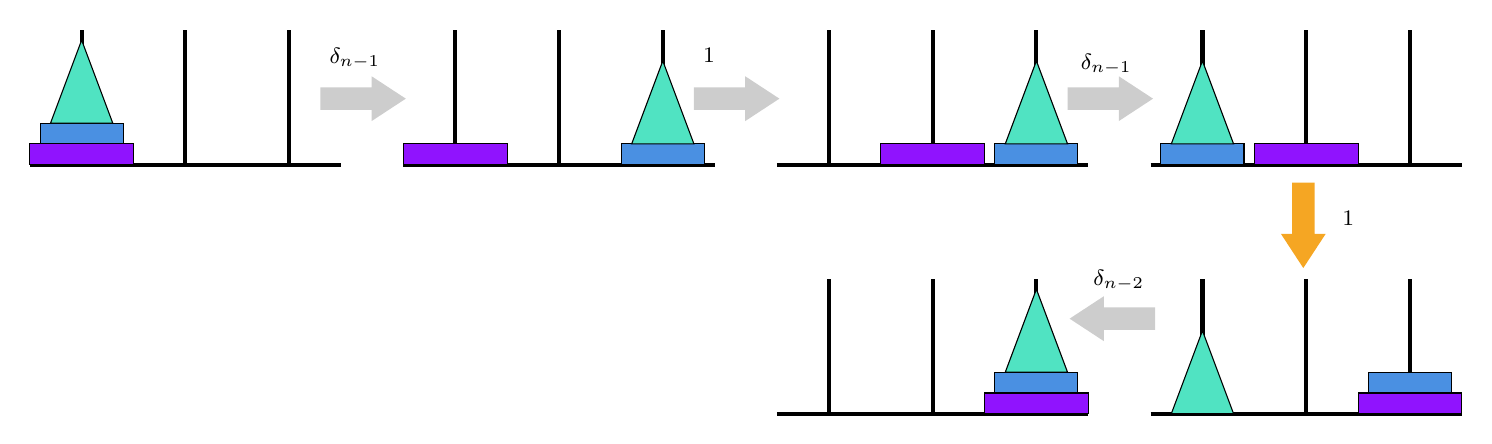
\begin{tikzpicture}[x=0.75pt,y=0.75pt,yscale=-1,xscale=1]
%uncomment if require: \path (0,285); %set diagram left start at 0, and has height of 285

%Straight Lines [id:da9072166137664734] 
\draw [line width=1.5]    (75,65) -- (75,0) ;
%Straight Lines [id:da1224816856441382] 
\draw [line width=1.5]    (125,65) -- (125,0) ;
%Straight Lines [id:da9296951412204004] 
\draw [line width=1.5]    (25,65) -- (25,0) ;
%Straight Lines [id:da28206094793705727] 
\draw [line width=1.5]    (0,65) -- (150,65) ;
%Shape: Rectangle [id:dp41711804875701697] 
\draw  [fill={rgb, 255:red, 74; green, 144; blue, 226 }  ,fill opacity=1 ] (5,45) -- (45,45) -- (45,55) -- (5,55) -- cycle ;
%Shape: Rectangle [id:dp1424378187144093] 
\draw  [fill={rgb, 255:red, 144; green, 19; blue, 254 }  ,fill opacity=1 ] (0,55) -- (50,55) -- (50,65) -- (0,65) -- cycle ;
%Shape: Triangle [id:dp7107841946620197] 
\draw  [fill={rgb, 255:red, 80; green, 227; blue, 194 }  ,fill opacity=1 ] (25,5) -- (40,45) -- (10,45) -- cycle ;
%Straight Lines [id:da5880650314649862] 
\draw [line width=1.5]    (255,65) -- (255,0) ;
%Straight Lines [id:da6574901990530537] 
\draw [line width=1.5]    (305,65) -- (305,0) ;
%Straight Lines [id:da7449012400683113] 
\draw [line width=1.5]    (205,65) -- (205,0) ;
%Straight Lines [id:da10297918912747628] 
\draw [line width=1.5]    (180,65) -- (330,65) ;
%Shape: Rectangle [id:dp6417608264148627] 
\draw  [fill={rgb, 255:red, 74; green, 144; blue, 226 }  ,fill opacity=1 ] (285,55) -- (325,55) -- (325,65) -- (285,65) -- cycle ;
%Shape: Rectangle [id:dp4558502187218114] 
\draw  [fill={rgb, 255:red, 144; green, 19; blue, 254 }  ,fill opacity=1 ] (180,55) -- (230,55) -- (230,65) -- (180,65) -- cycle ;
%Shape: Triangle [id:dp9908124419696638] 
\draw  [fill={rgb, 255:red, 80; green, 227; blue, 194 }  ,fill opacity=1 ] (305,15) -- (320,55) -- (290,55) -- cycle ;
%Straight Lines [id:da9444361295639931] 
\draw [line width=1.5]    (435,65) -- (435,0) ;
%Straight Lines [id:da5972635245511209] 
\draw [line width=1.5]    (485,65) -- (485,0) ;
%Straight Lines [id:da19575385527431766] 
\draw [line width=1.5]    (385,65) -- (385,0) ;
%Straight Lines [id:da923803362305267] 
\draw [line width=1.5]    (360,65) -- (510,65) ;
%Shape: Rectangle [id:dp688792399229569] 
\draw  [fill={rgb, 255:red, 74; green, 144; blue, 226 }  ,fill opacity=1 ] (465,55) -- (505,55) -- (505,65) -- (465,65) -- cycle ;
%Shape: Rectangle [id:dp5127560940618978] 
\draw  [fill={rgb, 255:red, 144; green, 19; blue, 254 }  ,fill opacity=1 ] (410,55) -- (460,55) -- (460,65) -- (410,65) -- cycle ;
%Shape: Triangle [id:dp7852790328313064] 
\draw  [fill={rgb, 255:red, 80; green, 227; blue, 194 }  ,fill opacity=1 ] (485,15) -- (500,55) -- (470,55) -- cycle ;
%Straight Lines [id:da5262851477333097] 
\draw [line width=1.5]    (615,65) -- (615,0) ;
%Straight Lines [id:da1464818021293528] 
\draw [line width=1.5]    (665,65) -- (665,0) ;
%Straight Lines [id:da5395186142286472] 
\draw [line width=1.5]    (565,65) -- (565,0) ;
%Straight Lines [id:da03606839773715609] 
\draw [line width=1.5]    (540,65) -- (690,65) ;
%Shape: Rectangle [id:dp16371770706432076] 
\draw  [fill={rgb, 255:red, 74; green, 144; blue, 226 }  ,fill opacity=1 ] (545,55) -- (585,55) -- (585,65) -- (545,65) -- cycle ;
%Shape: Rectangle [id:dp9064774256482331] 
\draw  [fill={rgb, 255:red, 144; green, 19; blue, 254 }  ,fill opacity=1 ] (590,55) -- (640,55) -- (640,65) -- (590,65) -- cycle ;
%Shape: Triangle [id:dp11181531728662497] 
\draw  [fill={rgb, 255:red, 80; green, 227; blue, 194 }  ,fill opacity=1 ] (565,15) -- (580,55) -- (550,55) -- cycle ;
%Right Arrow [id:dp6638650136928763] 
\draw  [draw opacity=0][fill={rgb, 255:red, 155; green, 155; blue, 155 }  ,fill opacity=0.5 ] (140,27.81) -- (164.71,27.81) -- (164.71,22.41) -- (181.18,33.2) -- (164.71,44) -- (164.71,38.6) -- (140,38.6) -- cycle ;
%Right Arrow [id:dp651558646758003] 
\draw  [draw opacity=0][fill={rgb, 255:red, 155; green, 155; blue, 155 }  ,fill opacity=0.5 ] (320,27.81) -- (344.71,27.81) -- (344.71,22.41) -- (361.18,33.2) -- (344.71,44) -- (344.71,38.6) -- (320,38.6) -- cycle ;
%Right Arrow [id:dp5809109935236172] 
\draw  [draw opacity=0][fill={rgb, 255:red, 155; green, 155; blue, 155 }  ,fill opacity=0.5 ] (500,27.81) -- (524.71,27.81) -- (524.71,22.41) -- (541.18,33.2) -- (524.71,44) -- (524.71,38.6) -- (500,38.6) -- cycle ;
%Straight Lines [id:da7229073696843578] 
\draw [line width=1.5]    (615,185) -- (615,120) ;
%Straight Lines [id:da04941429244465634] 
\draw [line width=1.5]    (665,185) -- (665,120) ;
%Straight Lines [id:da5468904048744319] 
\draw [line width=1.5]    (565,185) -- (565,120) ;
%Straight Lines [id:da0339738764262969] 
\draw [line width=1.5]    (540,185) -- (690,185) ;
%Shape: Rectangle [id:dp4369193219648857] 
\draw  [fill={rgb, 255:red, 74; green, 144; blue, 226 }  ,fill opacity=1 ] (645,165) -- (685,165) -- (685,175) -- (645,175) -- cycle ;
%Shape: Rectangle [id:dp01824550505442102] 
\draw  [fill={rgb, 255:red, 144; green, 19; blue, 254 }  ,fill opacity=1 ] (640,175) -- (690,175) -- (690,185) -- (640,185) -- cycle ;
%Shape: Triangle [id:dp482256539179293] 
\draw  [fill={rgb, 255:red, 80; green, 227; blue, 194 }  ,fill opacity=1 ] (565,145) -- (580,185) -- (550,185) -- cycle ;
%Straight Lines [id:da020449099543042415] 
\draw [line width=1.5]    (435,185) -- (435,120) ;
%Straight Lines [id:da3748411097269986] 
\draw [line width=1.5]    (485,185) -- (485,120) ;
%Straight Lines [id:da27173544436284636] 
\draw [line width=1.5]    (385,185) -- (385,120) ;
%Straight Lines [id:da10026896177229605] 
\draw [line width=1.5]    (360,185) -- (510,185) ;
%Shape: Rectangle [id:dp8859932119577489] 
\draw  [fill={rgb, 255:red, 74; green, 144; blue, 226 }  ,fill opacity=1 ] (465,165) -- (505,165) -- (505,175) -- (465,175) -- cycle ;
%Shape: Rectangle [id:dp3627054279813229] 
\draw  [fill={rgb, 255:red, 144; green, 19; blue, 254 }  ,fill opacity=1 ] (460,175) -- (510,175) -- (510,185) -- (460,185) -- cycle ;
%Shape: Triangle [id:dp49828025769446516] 
\draw  [fill={rgb, 255:red, 80; green, 227; blue, 194 }  ,fill opacity=1 ] (485,125) -- (500,165) -- (470,165) -- cycle ;
%Right Arrow [id:dp885046570936197] 
\draw  [draw opacity=0][fill={rgb, 255:red, 245; green, 166; blue, 35 }  ,fill opacity=1 ] (618.99,73.61) -- (618.99,98.32) -- (624.39,98.32) -- (613.59,114.8) -- (602.8,98.32) -- (608.19,98.32) -- (608.19,73.61) -- cycle ;
%Right Arrow [id:dp20340556434683443] 
\draw  [draw opacity=0][fill={rgb, 255:red, 155; green, 155; blue, 155 }  ,fill opacity=0.5 ] (542.18,144.6) -- (517.47,144.6) -- (517.47,150) -- (501,139.2) -- (517.47,128.41) -- (517.47,133.81) -- (542.18,133.81) -- cycle ;

% Text Node
\draw (143.18,7.4) node [anchor=north west][inner sep=0.75pt]  [font=\footnotesize]  {$\delta_{n-1}$};
% Text Node
\draw (323.18,7.4) node [anchor=north west][inner sep=0.75pt]  [font=\footnotesize]  {$1$};
% Text Node
\draw (511.18,114.4) node [anchor=north west][inner sep=0.75pt]  [font=\footnotesize]  {$\delta_{n-2}$};
% Text Node
\draw (631.18,86.4) node [anchor=north west][inner sep=0.75pt]  [font=\footnotesize]  {$1$};
% Text Node
\draw (505.18,10.4) node [anchor=north west][inner sep=0.75pt]  [font=\footnotesize]  {$\delta_{n-1}$};


\end{tikzpicture}
    \caption{Illustration of the procedure used to solve the Pell Tower for $n \geq 2$ discs}
    \label{fig:pell}
\end{figure}

Giving that $ P_{n}=\dfrac {\left(1+{\sqrt {2}}\right)^{n}-\left(1-{\sqrt {2}}\right)^{n}}{2{\sqrt {2}}}$, then we have the following. 

\begin{corollary}
    For all $n\geq 0$, we have 
    \begin{equation}
        \delta_{n}=\dfrac {\left(1+{\sqrt {2}}\right)^{n+1}-\left(1-{\sqrt {2}}\right)^{n+1}}{2{\sqrt {2}}}-1.
    \end{equation}
\end{corollary}


\begin{algorithm}[H]
\caption{Solution of the Tower of Pell}
\label{Alg:Pell}
\begin{algorithmic}[1]
\Procedure{Pell}{$n,i,j$}
\State $k:=6-i-j;$
\If{$n=1$}
\State move disc $1$ from peg $i$ to peg $j$;
\Else
\State \textsc{Pell}($n-1,i,j$);
\State move disc  $n$  to peg $k$;
\State \textsc{Pell}($n-1,j,i$);
\State move discs $n$ and $n-1$ simultaneously  to peg $j$ using Magic move;
\State \textsc{Pell}($n-2,i,j$);

\EndIf
\EndProcedure
\end{algorithmic}
\end{algorithm}


\section{Remarks about the four variants}
In contrast to the Towers of Fibonacci and Lucas for which the optimal solutions are unique, the optimal solutions of the Towers of Jacobsthal and Pell are not unique. Figure \ref{fig:jaco_optimal_solution_3} (resp. \ref{fig:pell_optimal_solution_3}) shows the optimal solution for of the Tower of Jacobsthal (resp. Pell) for $n=3$ discs, in move number $2$ (resp. $7$), discs $2$ and $1$ was moved simultaneously using a Magic move to peg $2$, then in the next move, disc $1$ was moved to peg $1$ (resp. $3$). However, move number $2$ (resp. $7$) can be changed by a classical move of disc $2$  to peg $2$, and then move number $3$ will be a move of disc $1$ from peg $3$ (resp. $1$) to peg $1$ (resp. $3$). These new changes will not change the length of the final solution. Hence, the optimal solution of the Tower of Jacobsthal (resp. Pell) is not unique. 

\begin{corollary}
    For all $n\geq 0$, we have 
    \begin{equation*}
        \alpha_{n} \leq \beta_{n}\leq  \gamma_{n}\leq \delta_{n}.
    \end{equation*}

\end{corollary}

\begin{table}[H]
\centering
\begin{tabular}{@{}lllllllllll@{}}
\toprule
$n$       & 0 & 1 & 2 & 3  & 4  & 5  & 6   & 7   & 8   & $\cdots$ \\ \midrule
$\alpha_{n}$   & 0 & 1 & 2 & 4 & 7 & 12 & 20 & 33 & 54 & $\cdots$ \\
$\beta_{n}$   & 0 & 2 & 3 & 6 & 10 & 17 & 28 & 46 & 75 & $\cdots$ \\ 
$\gamma_{n}$   & 0 & 1 & 4 & 9  & 20 & 41 & 84 & 169 & 340 & $\cdots$ \\

$\delta_{n}$   & 0 & 1 & 4 & 11 & 28 & 69 & 168 & 407 & 984 & $\cdots$ \\\bottomrule



\end{tabular}
\caption{A comparison between the four sequences $\alpha_{n}$, $\beta_{n}$, $\gamma_{n}$, and $\delta_{n}$}
\end{table}



\begin{remark}
     Equivalent sequences in the Online Encyclopedia of Integer Sequences   \cite{OEIS}.
    \begin{align}
        \alpha_{n}&=A000071(n),\quad \forall n\geq 0;\\
        \beta_{n}&=A001610(n),\quad \forall n\geq 0;\\
        \gamma_{n}&=A084639(n),\quad \forall n\geq 0;\\
        \delta_{n}&=A005409(n),\quad \forall n\geq 1.
    \end{align}
\end{remark}


  

 


\section{The associated graphs  }
Similarly to the Hanoi graph  $H_{n}$ associated with the classical Tower of Hanoi with $n\geq 1$ discs (see \cite[see Section 2.3]{hinz2018tower} for more about these graphs), the Towers of Fibonacci, Lucas, Pell, and Jacobsthal can each be associated to a class of graphs, which we call respectively,  Fibonacci-Tower graphs, Lucas-Tower graphs, Jacobsthal-Tower graphs, and Pell-Tower graphs, respectively. In this section, we present these new four classes of graphs, and we initiate the study of the particular class, the Fibonacci-Tower graphs.




Let $\mathcal{F}_{n}$ be the graph associated with the Tower of Fibonacci problem with $n\geq 1$ discs, called the Fibonacci-Tower graph, where $V(\mathcal{F}_{n})=V(H_{n})$ is the set of all possible $3^{n}$ states of the Tower of Hanoi, and arc $(u,v)$ exists in $A(\mathcal{F}_{n})$ if and only if the state $v$ can be reached from the state $u$ using one legal move (a classical or a Magic move). Every vertex (state)  $u\in V_{n}$ is represented  as an $n$-tuple,   i.e.,  $u = u_{n}\cdots u_{1}\in T^{n}$, where $u_{d}\in T=\{1,2,3\}$ is the peg on which disc $d\in[n]$ is lying in corresponding state.  




In contrast to    Hanoi graphs $H_{n}$,    Fibonacci-Tower graphs are oriented, since the Magic moves are not reversible. Figure  \ref{fig:fibo_graph2and3}  shows   the Fibonacci-Tower graphs $\mathcal{F}_{2}$ and $\mathcal{F}_{3}$, where the arcs colored in blue and red correspond to Magic moves of discs $2$ and $3$, respectively, and line
segments stand for arcs going both ways.

\begin{figure}[H]
    \centering
    

\tikzset{every picture/.style={line width=0.75pt}} %set default line width to 0.75pt        

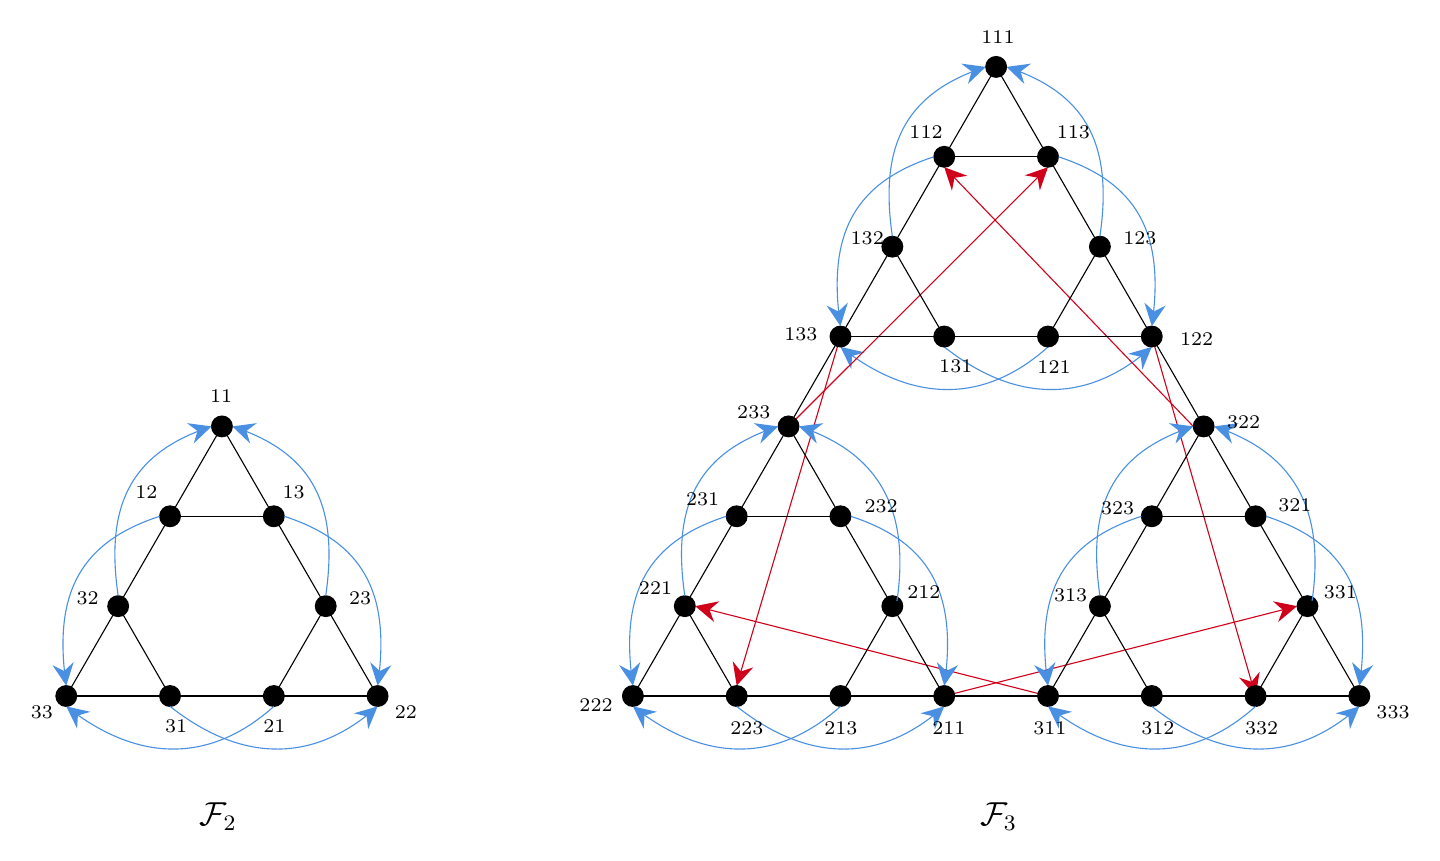
\begin{tikzpicture}[x=0.75pt,y=0.75pt,yscale=-1,xscale=1]
%uncomment if require: \path (0,544); %set diagram left start at 0, and has height of 544

%Straight Lines [id:da8384395596674512] 
\draw    (97,245.75) -- (147,245.75) ;
%Straight Lines [id:da7774669713501521] 
\draw    (122,202.45) -- (147,245.75) ;
%Straight Lines [id:da4671082972773417] 
\draw    (122,202.45) -- (97,245.75) ;
%Shape: Circle [id:dp7207253017065209] 
\draw  [fill={rgb, 255:red, 0; green, 0; blue, 0 }  ,fill opacity=1 ] (117,202.45) .. controls (117,199.69) and (119.24,197.45) .. (122,197.45) .. controls (124.76,197.45) and (127,199.69) .. (127,202.45) .. controls (127,205.21) and (124.76,207.45) .. (122,207.45) .. controls (119.24,207.45) and (117,205.21) .. (117,202.45) -- cycle ;
%Shape: Circle [id:dp7137426704333445] 
\draw  [fill={rgb, 255:red, 0; green, 0; blue, 0 }  ,fill opacity=1 ] (92,245.75) .. controls (92,242.99) and (94.24,240.75) .. (97,240.75) .. controls (99.76,240.75) and (102,242.99) .. (102,245.75) .. controls (102,248.51) and (99.76,250.75) .. (97,250.75) .. controls (94.24,250.75) and (92,248.51) .. (92,245.75) -- cycle ;
%Shape: Circle [id:dp11761952199405767] 
\draw  [fill={rgb, 255:red, 0; green, 0; blue, 0 }  ,fill opacity=1 ] (142,245.75) .. controls (142,242.99) and (144.24,240.75) .. (147,240.75) .. controls (149.76,240.75) and (152,242.99) .. (152,245.75) .. controls (152,248.51) and (149.76,250.75) .. (147,250.75) .. controls (144.24,250.75) and (142,248.51) .. (142,245.75) -- cycle ;
%Straight Lines [id:da6791984586569166] 
\draw    (97,245.75) -- (72,289.05) ;
%Straight Lines [id:da6026357097740973] 
\draw    (72,289.05) -- (47,332.35) ;
%Straight Lines [id:da14079094844667517] 
\draw    (147,245.75) -- (172,289.05) ;
%Straight Lines [id:da22761362978787836] 
\draw    (172,289.05) -- (197,332.35) ;
%Straight Lines [id:da5021899485755712] 
\draw    (172,289.05) -- (147,332.35) ;
%Straight Lines [id:da4587340129740831] 
\draw    (72,289.05) -- (97,332.35) ;
%Straight Lines [id:da7083194557126602] 
\draw    (47,332.35) -- (97,332.35) ;
%Straight Lines [id:da346171688588911] 
\draw    (147,332.35) -- (197,332.35) ;
%Straight Lines [id:da11576866377740647] 
\draw    (97,332.35) -- (147,332.35) ;
%Shape: Circle [id:dp02502659118488837] 
\draw  [fill={rgb, 255:red, 0; green, 0; blue, 0 }  ,fill opacity=1 ] (192,332.35) .. controls (192,329.59) and (194.24,327.35) .. (197,327.35) .. controls (199.76,327.35) and (202,329.59) .. (202,332.35) .. controls (202,335.11) and (199.76,337.35) .. (197,337.35) .. controls (194.24,337.35) and (192,335.11) .. (192,332.35) -- cycle ;
%Shape: Circle [id:dp4179202845406875] 
\draw  [fill={rgb, 255:red, 0; green, 0; blue, 0 }  ,fill opacity=1 ] (142,332.35) .. controls (142,329.59) and (144.24,327.35) .. (147,327.35) .. controls (149.76,327.35) and (152,329.59) .. (152,332.35) .. controls (152,335.11) and (149.76,337.35) .. (147,337.35) .. controls (144.24,337.35) and (142,335.11) .. (142,332.35) -- cycle ;
%Shape: Circle [id:dp5490131229614685] 
\draw  [fill={rgb, 255:red, 0; green, 0; blue, 0 }  ,fill opacity=1 ] (167,289.05) .. controls (167,286.29) and (169.24,284.05) .. (172,284.05) .. controls (174.76,284.05) and (177,286.29) .. (177,289.05) .. controls (177,291.81) and (174.76,294.05) .. (172,294.05) .. controls (169.24,294.05) and (167,291.81) .. (167,289.05) -- cycle ;
%Shape: Circle [id:dp9089558193262102] 
\draw  [fill={rgb, 255:red, 0; green, 0; blue, 0 }  ,fill opacity=1 ] (92,332.35) .. controls (92,329.59) and (94.24,327.35) .. (97,327.35) .. controls (99.76,327.35) and (102,329.59) .. (102,332.35) .. controls (102,335.11) and (99.76,337.35) .. (97,337.35) .. controls (94.24,337.35) and (92,335.11) .. (92,332.35) -- cycle ;
%Shape: Circle [id:dp08364253553168832] 
\draw  [fill={rgb, 255:red, 0; green, 0; blue, 0 }  ,fill opacity=1 ] (42,332.35) .. controls (42,329.59) and (44.24,327.35) .. (47,327.35) .. controls (49.76,327.35) and (52,329.59) .. (52,332.35) .. controls (52,335.11) and (49.76,337.35) .. (47,337.35) .. controls (44.24,337.35) and (42,335.11) .. (42,332.35) -- cycle ;
%Shape: Circle [id:dp13422487653631987] 
\draw  [fill={rgb, 255:red, 0; green, 0; blue, 0 }  ,fill opacity=1 ] (67,289.05) .. controls (67,286.29) and (69.24,284.05) .. (72,284.05) .. controls (74.76,284.05) and (77,286.29) .. (77,289.05) .. controls (77,291.81) and (74.76,294.05) .. (72,294.05) .. controls (69.24,294.05) and (67,291.81) .. (67,289.05) -- cycle ;
%Curve Lines [id:da016959333505828456] 
\draw [color={rgb, 255:red, 74; green, 144; blue, 226 }  ,draw opacity=1 ]   (152,245.75) .. controls (189.51,258.01) and (202.96,281.83) .. (197.37,324.7) ;
\draw [shift={(197,327.35)}, rotate = 278.3] [fill={rgb, 255:red, 74; green, 144; blue, 226 }  ,fill opacity=1 ][line width=0.08]  [draw opacity=0] (10.72,-5.15) -- (0,0) -- (10.72,5.15) -- (7.12,0) -- cycle    ;
%Curve Lines [id:da29340677572936613] 
\draw [color={rgb, 255:red, 74; green, 144; blue, 226 }  ,draw opacity=1 ]   (130.38,203.61) .. controls (166.05,216.45) and (178.31,240.84) .. (172,284.05) ;
\draw [shift={(127,202.45)}, rotate = 18.1] [fill={rgb, 255:red, 74; green, 144; blue, 226 }  ,fill opacity=1 ][line width=0.08]  [draw opacity=0] (10.72,-5.15) -- (0,0) -- (10.72,5.15) -- (7.12,0) -- cycle    ;
%Curve Lines [id:da6699458233969207] 
\draw [color={rgb, 255:red, 74; green, 144; blue, 226 }  ,draw opacity=1 ]   (113.62,203.61) .. controls (77.95,216.45) and (65.7,240.84) .. (72,284.05) ;
\draw [shift={(117,202.45)}, rotate = 161.9] [fill={rgb, 255:red, 74; green, 144; blue, 226 }  ,fill opacity=1 ][line width=0.08]  [draw opacity=0] (10.72,-5.15) -- (0,0) -- (10.72,5.15) -- (7.12,0) -- cycle    ;
%Curve Lines [id:da8565950672282625] 
\draw [color={rgb, 255:red, 74; green, 144; blue, 226 }  ,draw opacity=1 ]   (92,245.75) .. controls (54.49,258.01) and (41.04,281.83) .. (46.63,324.7) ;
\draw [shift={(47,327.35)}, rotate = 261.7] [fill={rgb, 255:red, 74; green, 144; blue, 226 }  ,fill opacity=1 ][line width=0.08]  [draw opacity=0] (10.72,-5.15) -- (0,0) -- (10.72,5.15) -- (7.12,0) -- cycle    ;
%Curve Lines [id:da9794624496543418] 
\draw [color={rgb, 255:red, 74; green, 144; blue, 226 }  ,draw opacity=1 ]   (147,337.35) .. controls (117.63,363.71) and (83.71,365.2) .. (49.12,338.99) ;
\draw [shift={(47,337.35)}, rotate = 38.3] [fill={rgb, 255:red, 74; green, 144; blue, 226 }  ,fill opacity=1 ][line width=0.08]  [draw opacity=0] (10.72,-5.15) -- (0,0) -- (10.72,5.15) -- (7.12,0) -- cycle    ;
%Curve Lines [id:da11758545037782997] 
\draw [color={rgb, 255:red, 74; green, 144; blue, 226 }  ,draw opacity=1 ]   (194.29,339.7) .. controls (164.95,364.28) and (131.27,364.42) .. (97,337.35) ;
\draw [shift={(197,337.35)}, rotate = 138.1] [fill={rgb, 255:red, 74; green, 144; blue, 226 }  ,fill opacity=1 ][line width=0.08]  [draw opacity=0] (10.72,-5.15) -- (0,0) -- (10.72,5.15) -- (7.12,0) -- cycle    ;

%Curve Lines [id:da6425379829733171] 
\draw [color={rgb, 255:red, 74; green, 144; blue, 226 }  ,draw opacity=1 ]   (520,164.15) .. controls (490.63,190.5) and (456.71,192) .. (422.12,165.79) ;
\draw [shift={(420,164.15)}, rotate = 38.3] [fill={rgb, 255:red, 74; green, 144; blue, 226 }  ,fill opacity=1 ][line width=0.08]  [draw opacity=0] (10.72,-5.15) -- (0,0) -- (10.72,5.15) -- (7.12,0) -- cycle    ;
%Curve Lines [id:da7185195630041767] 
\draw [color={rgb, 255:red, 74; green, 144; blue, 226 }  ,draw opacity=1 ]   (567.29,166.5) .. controls (537.95,191.07) and (504.27,191.21) .. (470,164.15) ;
\draw [shift={(570,164.15)}, rotate = 138.1] [fill={rgb, 255:red, 74; green, 144; blue, 226 }  ,fill opacity=1 ][line width=0.08]  [draw opacity=0] (10.72,-5.15) -- (0,0) -- (10.72,5.15) -- (7.12,0) -- cycle    ;
%Straight Lines [id:da8530189738717202] 
\draw    (420,159.15) -- (395,202.45) ;
%Straight Lines [id:da8460537068681633] 
\draw    (570,159.15) -- (595,202.45) ;
%Straight Lines [id:da8380568395183166] 
\draw [color={rgb, 255:red, 208; green, 2; blue, 27 }  ,draw opacity=1 ]   (590,202.45) -- (472.08,79.71) ;
\draw [shift={(470,77.55)}, rotate = 46.15] [fill={rgb, 255:red, 208; green, 2; blue, 27 }  ,fill opacity=1 ][line width=0.08]  [draw opacity=0] (10.72,-5.15) -- (0,0) -- (10.72,5.15) -- (7.12,0) -- cycle    ;
%Straight Lines [id:da5969556080200338] 
\draw [color={rgb, 255:red, 208; green, 2; blue, 27 }  ,draw opacity=1 ]   (395,202.45) -- (517.88,79.67) ;
\draw [shift={(520,77.55)}, rotate = 135.02] [fill={rgb, 255:red, 208; green, 2; blue, 27 }  ,fill opacity=1 ][line width=0.08]  [draw opacity=0] (10.72,-5.15) -- (0,0) -- (10.72,5.15) -- (7.12,0) -- cycle    ;
%Straight Lines [id:da6826625916186193] 
\draw [color={rgb, 255:red, 208; green, 2; blue, 27 }  ,draw opacity=1 ]   (570,159.15) -- (619.17,329.47) ;
\draw [shift={(620,332.35)}, rotate = 253.9] [fill={rgb, 255:red, 208; green, 2; blue, 27 }  ,fill opacity=1 ][line width=0.08]  [draw opacity=0] (10.72,-5.15) -- (0,0) -- (10.72,5.15) -- (7.12,0) -- cycle    ;
%Straight Lines [id:da7398602419844795] 
\draw [color={rgb, 255:red, 208; green, 2; blue, 27 }  ,draw opacity=1 ]   (420,159.15) -- (370.85,324.48) ;
\draw [shift={(370,327.35)}, rotate = 286.55] [fill={rgb, 255:red, 208; green, 2; blue, 27 }  ,fill opacity=1 ][line width=0.08]  [draw opacity=0] (10.72,-5.15) -- (0,0) -- (10.72,5.15) -- (7.12,0) -- cycle    ;
%Straight Lines [id:da6806839396681874] 
\draw    (470,332.35) -- (520,332.35) ;
%Straight Lines [id:da8727251050528813] 
\draw [color={rgb, 255:red, 208; green, 2; blue, 27 }  ,draw opacity=1 ]   (520,332.35) -- (352.91,289.79) ;
\draw [shift={(350,289.05)}, rotate = 14.29] [fill={rgb, 255:red, 208; green, 2; blue, 27 }  ,fill opacity=1 ][line width=0.08]  [draw opacity=0] (10.72,-5.15) -- (0,0) -- (10.72,5.15) -- (7.12,0) -- cycle    ;
%Straight Lines [id:da9327393322666742] 
\draw [color={rgb, 255:red, 208; green, 2; blue, 27 }  ,draw opacity=1 ]   (470,332.35) -- (637.09,289.79) ;
\draw [shift={(640,289.05)}, rotate = 165.71] [fill={rgb, 255:red, 208; green, 2; blue, 27 }  ,fill opacity=1 ][line width=0.08]  [draw opacity=0] (10.72,-5.15) -- (0,0) -- (10.72,5.15) -- (7.12,0) -- cycle    ;
%Straight Lines [id:da1869416378787636] 
\draw    (470,72.55) -- (520,72.55) ;
%Straight Lines [id:da17698680439940762] 
\draw    (495,29.24) -- (520,72.55) ;
%Straight Lines [id:da9856444591557174] 
\draw    (495,29.24) -- (470,72.55) ;
%Shape: Circle [id:dp5221106208433797] 
\draw  [fill={rgb, 255:red, 0; green, 0; blue, 0 }  ,fill opacity=1 ] (490,29.24) .. controls (490,26.48) and (492.24,24.24) .. (495,24.24) .. controls (497.76,24.24) and (500,26.48) .. (500,29.24) .. controls (500,32.01) and (497.76,34.24) .. (495,34.24) .. controls (492.24,34.24) and (490,32.01) .. (490,29.24) -- cycle ;
%Shape: Circle [id:dp7050027612149852] 
\draw  [fill={rgb, 255:red, 0; green, 0; blue, 0 }  ,fill opacity=1 ] (465,72.55) .. controls (465,69.78) and (467.24,67.55) .. (470,67.55) .. controls (472.76,67.55) and (475,69.78) .. (475,72.55) .. controls (475,75.31) and (472.76,77.55) .. (470,77.55) .. controls (467.24,77.55) and (465,75.31) .. (465,72.55) -- cycle ;
%Shape: Circle [id:dp9188592261203201] 
\draw  [fill={rgb, 255:red, 0; green, 0; blue, 0 }  ,fill opacity=1 ] (515,72.55) .. controls (515,69.78) and (517.24,67.55) .. (520,67.55) .. controls (522.76,67.55) and (525,69.78) .. (525,72.55) .. controls (525,75.31) and (522.76,77.55) .. (520,77.55) .. controls (517.24,77.55) and (515,75.31) .. (515,72.55) -- cycle ;
%Straight Lines [id:da5093586282530966] 
\draw    (470,72.55) -- (445,115.85) ;
%Straight Lines [id:da15596917956034484] 
\draw    (445,115.85) -- (420,159.15) ;
%Straight Lines [id:da5148217856254123] 
\draw    (520,72.55) -- (545,115.85) ;
%Straight Lines [id:da5287497208822929] 
\draw    (545,115.85) -- (570,159.15) ;
%Straight Lines [id:da9481059266844023] 
\draw    (545,115.85) -- (520,159.15) ;
%Straight Lines [id:da2397945264968082] 
\draw    (445,115.85) -- (470,159.15) ;
%Straight Lines [id:da4418765002820626] 
\draw    (420,159.15) -- (470,159.15) ;
%Straight Lines [id:da4484345012774731] 
\draw    (520,159.15) -- (570,159.15) ;
%Straight Lines [id:da3513707342229129] 
\draw    (470,159.15) -- (520,159.15) ;
%Shape: Circle [id:dp5490222758150483] 
\draw  [fill={rgb, 255:red, 0; green, 0; blue, 0 }  ,fill opacity=1 ] (565,159.15) .. controls (565,156.39) and (567.24,154.15) .. (570,154.15) .. controls (572.76,154.15) and (575,156.39) .. (575,159.15) .. controls (575,161.91) and (572.76,164.15) .. (570,164.15) .. controls (567.24,164.15) and (565,161.91) .. (565,159.15) -- cycle ;
%Shape: Circle [id:dp18061923760014453] 
\draw  [fill={rgb, 255:red, 0; green, 0; blue, 0 }  ,fill opacity=1 ] (515,159.15) .. controls (515,156.39) and (517.24,154.15) .. (520,154.15) .. controls (522.76,154.15) and (525,156.39) .. (525,159.15) .. controls (525,161.91) and (522.76,164.15) .. (520,164.15) .. controls (517.24,164.15) and (515,161.91) .. (515,159.15) -- cycle ;
%Shape: Circle [id:dp7038778171421551] 
\draw  [fill={rgb, 255:red, 0; green, 0; blue, 0 }  ,fill opacity=1 ] (540,115.85) .. controls (540,113.09) and (542.24,110.85) .. (545,110.85) .. controls (547.76,110.85) and (550,113.09) .. (550,115.85) .. controls (550,118.61) and (547.76,120.85) .. (545,120.85) .. controls (542.24,120.85) and (540,118.61) .. (540,115.85) -- cycle ;
%Shape: Circle [id:dp2332955159751413] 
\draw  [fill={rgb, 255:red, 0; green, 0; blue, 0 }  ,fill opacity=1 ] (465,159.15) .. controls (465,156.39) and (467.24,154.15) .. (470,154.15) .. controls (472.76,154.15) and (475,156.39) .. (475,159.15) .. controls (475,161.91) and (472.76,164.15) .. (470,164.15) .. controls (467.24,164.15) and (465,161.91) .. (465,159.15) -- cycle ;
%Shape: Circle [id:dp4000581399930456] 
\draw  [fill={rgb, 255:red, 0; green, 0; blue, 0 }  ,fill opacity=1 ] (415,159.15) .. controls (415,156.39) and (417.24,154.15) .. (420,154.15) .. controls (422.76,154.15) and (425,156.39) .. (425,159.15) .. controls (425,161.91) and (422.76,164.15) .. (420,164.15) .. controls (417.24,164.15) and (415,161.91) .. (415,159.15) -- cycle ;
%Shape: Circle [id:dp25721289033377803] 
\draw  [fill={rgb, 255:red, 0; green, 0; blue, 0 }  ,fill opacity=1 ] (440,115.85) .. controls (440,113.09) and (442.24,110.85) .. (445,110.85) .. controls (447.76,110.85) and (450,113.09) .. (450,115.85) .. controls (450,118.61) and (447.76,120.85) .. (445,120.85) .. controls (442.24,120.85) and (440,118.61) .. (440,115.85) -- cycle ;
%Curve Lines [id:da7468723768862806] 
\draw [color={rgb, 255:red, 74; green, 144; blue, 226 }  ,draw opacity=1 ]   (525,72.55) .. controls (562.51,84.8) and (575.96,108.63) .. (570.37,151.5) ;
\draw [shift={(570,154.15)}, rotate = 278.3] [fill={rgb, 255:red, 74; green, 144; blue, 226 }  ,fill opacity=1 ][line width=0.08]  [draw opacity=0] (10.72,-5.15) -- (0,0) -- (10.72,5.15) -- (7.12,0) -- cycle    ;
%Curve Lines [id:da3987962719917233] 
\draw [color={rgb, 255:red, 74; green, 144; blue, 226 }  ,draw opacity=1 ]   (503.38,30.4) .. controls (539.05,43.24) and (551.3,67.64) .. (545,110.85) ;
\draw [shift={(500,29.24)}, rotate = 18.1] [fill={rgb, 255:red, 74; green, 144; blue, 226 }  ,fill opacity=1 ][line width=0.08]  [draw opacity=0] (10.72,-5.15) -- (0,0) -- (10.72,5.15) -- (7.12,0) -- cycle    ;
%Curve Lines [id:da9625339728305051] 
\draw [color={rgb, 255:red, 74; green, 144; blue, 226 }  ,draw opacity=1 ]   (486.62,30.4) .. controls (450.95,43.24) and (438.7,67.64) .. (445,110.85) ;
\draw [shift={(490,29.24)}, rotate = 161.9] [fill={rgb, 255:red, 74; green, 144; blue, 226 }  ,fill opacity=1 ][line width=0.08]  [draw opacity=0] (10.72,-5.15) -- (0,0) -- (10.72,5.15) -- (7.12,0) -- cycle    ;
%Curve Lines [id:da3180105393226491] 
\draw [color={rgb, 255:red, 74; green, 144; blue, 226 }  ,draw opacity=1 ]   (465,72.55) .. controls (427.49,84.8) and (414.04,108.63) .. (419.63,151.5) ;
\draw [shift={(420,154.15)}, rotate = 261.7] [fill={rgb, 255:red, 74; green, 144; blue, 226 }  ,fill opacity=1 ][line width=0.08]  [draw opacity=0] (10.72,-5.15) -- (0,0) -- (10.72,5.15) -- (7.12,0) -- cycle    ;
%Straight Lines [id:da6507171399802465] 
\draw    (395,202.45) -- (370,245.75) ;
%Straight Lines [id:da22373542875453567] 
\draw    (395,202.45) -- (420,245.75) ;
%Straight Lines [id:da758467241178499] 
\draw    (595,202.45) -- (620,245.75) ;
%Straight Lines [id:da6533645820723712] 
\draw    (595,202.45) -- (570,245.75) ;
%Straight Lines [id:da8782914307658527] 
\draw    (570,245.75) -- (545,289.05) ;
%Straight Lines [id:da768315614734357] 
\draw    (545,289.05) -- (520,332.35) ;
%Straight Lines [id:da9005102826634295] 
\draw    (420,245.75) -- (445,289.05) ;
%Straight Lines [id:da8134232694484513] 
\draw    (445,289.05) -- (470,332.35) ;
%Straight Lines [id:da26890044772498745] 
\draw    (620,245.75) -- (645,289.05) ;
%Straight Lines [id:da8958411746420687] 
\draw    (645,289.05) -- (670,332.35) ;
%Straight Lines [id:da5380245634457499] 
\draw    (370,245.75) -- (345,289.05) ;
%Straight Lines [id:da8897506665246622] 
\draw    (345,289.05) -- (320,332.35) ;
%Straight Lines [id:da8508914353614696] 
\draw    (320,332.35) -- (370,332.35) ;
%Straight Lines [id:da37729863567085387] 
\draw    (370,332.35) -- (420,332.35) ;
%Straight Lines [id:da2877162624594727] 
\draw    (420,332.35) -- (470,332.35) ;
%Straight Lines [id:da9022682680706016] 
\draw    (520,332.35) -- (570,332.35) ;
%Straight Lines [id:da8208582985668831] 
\draw    (570,332.35) -- (620,332.35) ;
%Straight Lines [id:da9911770566342615] 
\draw    (620,332.35) -- (670,332.35) ;
%Straight Lines [id:da8072208022787304] 
\draw    (570,245.75) -- (620,245.75) ;
%Straight Lines [id:da7391989893076167] 
\draw    (370,245.75) -- (420,245.75) ;
%Straight Lines [id:da9048155044363573] 
\draw    (345,289.05) -- (370,332.35) ;
%Straight Lines [id:da2482834332958357] 
\draw    (545,289.05) -- (570,332.35) ;
%Straight Lines [id:da6888016948857907] 
\draw    (445,289.05) -- (420,332.35) ;
%Straight Lines [id:da6827581082829226] 
\draw    (645,289.05) -- (620,332.35) ;
%Shape: Circle [id:dp575341052299229] 
\draw  [fill={rgb, 255:red, 0; green, 0; blue, 0 }  ,fill opacity=1 ] (590,202.45) .. controls (590,199.69) and (592.24,197.45) .. (595,197.45) .. controls (597.76,197.45) and (600,199.69) .. (600,202.45) .. controls (600,205.21) and (597.76,207.45) .. (595,207.45) .. controls (592.24,207.45) and (590,205.21) .. (590,202.45) -- cycle ;
%Shape: Circle [id:dp1609108544396034] 
\draw  [fill={rgb, 255:red, 0; green, 0; blue, 0 }  ,fill opacity=1 ] (615,245.75) .. controls (615,242.99) and (617.24,240.75) .. (620,240.75) .. controls (622.76,240.75) and (625,242.99) .. (625,245.75) .. controls (625,248.51) and (622.76,250.75) .. (620,250.75) .. controls (617.24,250.75) and (615,248.51) .. (615,245.75) -- cycle ;
%Shape: Circle [id:dp8595371723386391] 
\draw  [fill={rgb, 255:red, 0; green, 0; blue, 0 }  ,fill opacity=1 ] (640,289.05) .. controls (640,286.29) and (642.24,284.05) .. (645,284.05) .. controls (647.76,284.05) and (650,286.29) .. (650,289.05) .. controls (650,291.81) and (647.76,294.05) .. (645,294.05) .. controls (642.24,294.05) and (640,291.81) .. (640,289.05) -- cycle ;
%Shape: Circle [id:dp6023973743669484] 
\draw  [fill={rgb, 255:red, 0; green, 0; blue, 0 }  ,fill opacity=1 ] (665,332.35) .. controls (665,329.59) and (667.24,327.35) .. (670,327.35) .. controls (672.76,327.35) and (675,329.59) .. (675,332.35) .. controls (675,335.11) and (672.76,337.35) .. (670,337.35) .. controls (667.24,337.35) and (665,335.11) .. (665,332.35) -- cycle ;
%Shape: Circle [id:dp8728669403499232] 
\draw  [fill={rgb, 255:red, 0; green, 0; blue, 0 }  ,fill opacity=1 ] (615,332.35) .. controls (615,329.59) and (617.24,327.35) .. (620,327.35) .. controls (622.76,327.35) and (625,329.59) .. (625,332.35) .. controls (625,335.11) and (622.76,337.35) .. (620,337.35) .. controls (617.24,337.35) and (615,335.11) .. (615,332.35) -- cycle ;
%Shape: Circle [id:dp6845837729092683] 
\draw  [fill={rgb, 255:red, 0; green, 0; blue, 0 }  ,fill opacity=1 ] (565,332.35) .. controls (565,329.59) and (567.24,327.35) .. (570,327.35) .. controls (572.76,327.35) and (575,329.59) .. (575,332.35) .. controls (575,335.11) and (572.76,337.35) .. (570,337.35) .. controls (567.24,337.35) and (565,335.11) .. (565,332.35) -- cycle ;
%Shape: Circle [id:dp7335589881957478] 
\draw  [fill={rgb, 255:red, 0; green, 0; blue, 0 }  ,fill opacity=1 ] (515,332.35) .. controls (515,329.59) and (517.24,327.35) .. (520,327.35) .. controls (522.76,327.35) and (525,329.59) .. (525,332.35) .. controls (525,335.11) and (522.76,337.35) .. (520,337.35) .. controls (517.24,337.35) and (515,335.11) .. (515,332.35) -- cycle ;
%Shape: Circle [id:dp82058878443319] 
\draw  [fill={rgb, 255:red, 0; green, 0; blue, 0 }  ,fill opacity=1 ] (540,289.05) .. controls (540,286.29) and (542.24,284.05) .. (545,284.05) .. controls (547.76,284.05) and (550,286.29) .. (550,289.05) .. controls (550,291.81) and (547.76,294.05) .. (545,294.05) .. controls (542.24,294.05) and (540,291.81) .. (540,289.05) -- cycle ;
%Shape: Circle [id:dp01156027607965382] 
\draw  [fill={rgb, 255:red, 0; green, 0; blue, 0 }  ,fill opacity=1 ] (565,245.75) .. controls (565,242.99) and (567.24,240.75) .. (570,240.75) .. controls (572.76,240.75) and (575,242.99) .. (575,245.75) .. controls (575,248.51) and (572.76,250.75) .. (570,250.75) .. controls (567.24,250.75) and (565,248.51) .. (565,245.75) -- cycle ;
%Shape: Circle [id:dp7031480543781525] 
\draw  [fill={rgb, 255:red, 0; green, 0; blue, 0 }  ,fill opacity=1 ] (390,202.45) .. controls (390,199.69) and (392.24,197.45) .. (395,197.45) .. controls (397.76,197.45) and (400,199.69) .. (400,202.45) .. controls (400,205.21) and (397.76,207.45) .. (395,207.45) .. controls (392.24,207.45) and (390,205.21) .. (390,202.45) -- cycle ;
%Shape: Circle [id:dp825450944547842] 
\draw  [fill={rgb, 255:red, 0; green, 0; blue, 0 }  ,fill opacity=1 ] (415,245.75) .. controls (415,242.99) and (417.24,240.75) .. (420,240.75) .. controls (422.76,240.75) and (425,242.99) .. (425,245.75) .. controls (425,248.51) and (422.76,250.75) .. (420,250.75) .. controls (417.24,250.75) and (415,248.51) .. (415,245.75) -- cycle ;
%Shape: Circle [id:dp16567078848327554] 
\draw  [fill={rgb, 255:red, 0; green, 0; blue, 0 }  ,fill opacity=1 ] (440,289.05) .. controls (440,286.29) and (442.24,284.05) .. (445,284.05) .. controls (447.76,284.05) and (450,286.29) .. (450,289.05) .. controls (450,291.81) and (447.76,294.05) .. (445,294.05) .. controls (442.24,294.05) and (440,291.81) .. (440,289.05) -- cycle ;
%Shape: Circle [id:dp678677836673262] 
\draw  [fill={rgb, 255:red, 0; green, 0; blue, 0 }  ,fill opacity=1 ] (465,332.35) .. controls (465,329.59) and (467.24,327.35) .. (470,327.35) .. controls (472.76,327.35) and (475,329.59) .. (475,332.35) .. controls (475,335.11) and (472.76,337.35) .. (470,337.35) .. controls (467.24,337.35) and (465,335.11) .. (465,332.35) -- cycle ;
%Shape: Circle [id:dp8004750363745599] 
\draw  [fill={rgb, 255:red, 0; green, 0; blue, 0 }  ,fill opacity=1 ] (415,332.35) .. controls (415,329.59) and (417.24,327.35) .. (420,327.35) .. controls (422.76,327.35) and (425,329.59) .. (425,332.35) .. controls (425,335.11) and (422.76,337.35) .. (420,337.35) .. controls (417.24,337.35) and (415,335.11) .. (415,332.35) -- cycle ;
%Shape: Circle [id:dp717034320742677] 
\draw  [fill={rgb, 255:red, 0; green, 0; blue, 0 }  ,fill opacity=1 ] (365,332.35) .. controls (365,329.59) and (367.24,327.35) .. (370,327.35) .. controls (372.76,327.35) and (375,329.59) .. (375,332.35) .. controls (375,335.11) and (372.76,337.35) .. (370,337.35) .. controls (367.24,337.35) and (365,335.11) .. (365,332.35) -- cycle ;
%Shape: Circle [id:dp39395321893654933] 
\draw  [fill={rgb, 255:red, 0; green, 0; blue, 0 }  ,fill opacity=1 ] (315,332.35) .. controls (315,329.59) and (317.24,327.35) .. (320,327.35) .. controls (322.76,327.35) and (325,329.59) .. (325,332.35) .. controls (325,335.11) and (322.76,337.35) .. (320,337.35) .. controls (317.24,337.35) and (315,335.11) .. (315,332.35) -- cycle ;
%Shape: Circle [id:dp7822411186444644] 
\draw  [fill={rgb, 255:red, 0; green, 0; blue, 0 }  ,fill opacity=1 ] (340,289.05) .. controls (340,286.29) and (342.24,284.05) .. (345,284.05) .. controls (347.76,284.05) and (350,286.29) .. (350,289.05) .. controls (350,291.81) and (347.76,294.05) .. (345,294.05) .. controls (342.24,294.05) and (340,291.81) .. (340,289.05) -- cycle ;
%Shape: Circle [id:dp3195601689295524] 
\draw  [fill={rgb, 255:red, 0; green, 0; blue, 0 }  ,fill opacity=1 ] (365,245.75) .. controls (365,242.99) and (367.24,240.75) .. (370,240.75) .. controls (372.76,240.75) and (375,242.99) .. (375,245.75) .. controls (375,248.51) and (372.76,250.75) .. (370,250.75) .. controls (367.24,250.75) and (365,248.51) .. (365,245.75) -- cycle ;
%Curve Lines [id:da22933729143517456] 
\draw [color={rgb, 255:red, 74; green, 144; blue, 226 }  ,draw opacity=1 ]   (625,245.75) .. controls (662.51,258.01) and (675.96,281.83) .. (670.37,324.7) ;
\draw [shift={(670,327.35)}, rotate = 278.3] [fill={rgb, 255:red, 74; green, 144; blue, 226 }  ,fill opacity=1 ][line width=0.08]  [draw opacity=0] (10.72,-5.15) -- (0,0) -- (10.72,5.15) -- (7.12,0) -- cycle    ;
%Curve Lines [id:da4136118900953891] 
\draw [color={rgb, 255:red, 74; green, 144; blue, 226 }  ,draw opacity=1 ]   (603.38,203.61) .. controls (639.18,216.6) and (653.52,243.34) .. (647.21,286.55) ;
\draw [shift={(600,202.45)}, rotate = 18.1] [fill={rgb, 255:red, 74; green, 144; blue, 226 }  ,fill opacity=1 ][line width=0.08]  [draw opacity=0] (10.72,-5.15) -- (0,0) -- (10.72,5.15) -- (7.12,0) -- cycle    ;
%Curve Lines [id:da3630341364628784] 
\draw [color={rgb, 255:red, 74; green, 144; blue, 226 }  ,draw opacity=1 ]   (586.62,203.61) .. controls (550.95,216.45) and (538.7,240.84) .. (545,284.05) ;
\draw [shift={(590,202.45)}, rotate = 161.9] [fill={rgb, 255:red, 74; green, 144; blue, 226 }  ,fill opacity=1 ][line width=0.08]  [draw opacity=0] (10.72,-5.15) -- (0,0) -- (10.72,5.15) -- (7.12,0) -- cycle    ;
%Curve Lines [id:da09156538662040803] 
\draw [color={rgb, 255:red, 74; green, 144; blue, 226 }  ,draw opacity=1 ]   (386.62,203.61) .. controls (350.95,216.45) and (338.7,240.84) .. (345,284.05) ;
\draw [shift={(390,202.45)}, rotate = 161.9] [fill={rgb, 255:red, 74; green, 144; blue, 226 }  ,fill opacity=1 ][line width=0.08]  [draw opacity=0] (10.72,-5.15) -- (0,0) -- (10.72,5.15) -- (7.12,0) -- cycle    ;
%Curve Lines [id:da935218768640431] 
\draw [color={rgb, 255:red, 74; green, 144; blue, 226 }  ,draw opacity=1 ]   (425,245.75) .. controls (462.51,258.01) and (475.96,281.83) .. (470.37,324.7) ;
\draw [shift={(470,327.35)}, rotate = 278.3] [fill={rgb, 255:red, 74; green, 144; blue, 226 }  ,fill opacity=1 ][line width=0.08]  [draw opacity=0] (10.72,-5.15) -- (0,0) -- (10.72,5.15) -- (7.12,0) -- cycle    ;
%Curve Lines [id:da9326466428378315] 
\draw [color={rgb, 255:red, 74; green, 144; blue, 226 }  ,draw opacity=1 ]   (403.38,203.61) .. controls (439.18,216.6) and (453.52,243.34) .. (447.21,286.55) ;
\draw [shift={(400,202.45)}, rotate = 18.1] [fill={rgb, 255:red, 74; green, 144; blue, 226 }  ,fill opacity=1 ][line width=0.08]  [draw opacity=0] (10.72,-5.15) -- (0,0) -- (10.72,5.15) -- (7.12,0) -- cycle    ;
%Curve Lines [id:da5232157131447828] 
\draw [color={rgb, 255:red, 74; green, 144; blue, 226 }  ,draw opacity=1 ]   (365,245.75) .. controls (327.49,258.01) and (314.04,281.83) .. (319.63,324.7) ;
\draw [shift={(320,327.35)}, rotate = 261.7] [fill={rgb, 255:red, 74; green, 144; blue, 226 }  ,fill opacity=1 ][line width=0.08]  [draw opacity=0] (10.72,-5.15) -- (0,0) -- (10.72,5.15) -- (7.12,0) -- cycle    ;
%Curve Lines [id:da10488861143192074] 
\draw [color={rgb, 255:red, 74; green, 144; blue, 226 }  ,draw opacity=1 ]   (565,245.75) .. controls (527.49,258.01) and (514.04,281.83) .. (519.63,324.7) ;
\draw [shift={(520,327.35)}, rotate = 261.7] [fill={rgb, 255:red, 74; green, 144; blue, 226 }  ,fill opacity=1 ][line width=0.08]  [draw opacity=0] (10.72,-5.15) -- (0,0) -- (10.72,5.15) -- (7.12,0) -- cycle    ;
%Curve Lines [id:da2714359584862349] 
\draw [color={rgb, 255:red, 74; green, 144; blue, 226 }  ,draw opacity=1 ]   (667.29,339.7) .. controls (637.95,364.28) and (604.27,364.42) .. (570,337.35) ;
\draw [shift={(670,337.35)}, rotate = 138.1] [fill={rgb, 255:red, 74; green, 144; blue, 226 }  ,fill opacity=1 ][line width=0.08]  [draw opacity=0] (10.72,-5.15) -- (0,0) -- (10.72,5.15) -- (7.12,0) -- cycle    ;
%Curve Lines [id:da3870162054490216] 
\draw [color={rgb, 255:red, 74; green, 144; blue, 226 }  ,draw opacity=1 ]   (467.29,339.7) .. controls (437.95,364.28) and (404.27,364.42) .. (370,337.35) ;
\draw [shift={(470,337.35)}, rotate = 138.1] [fill={rgb, 255:red, 74; green, 144; blue, 226 }  ,fill opacity=1 ][line width=0.08]  [draw opacity=0] (10.72,-5.15) -- (0,0) -- (10.72,5.15) -- (7.12,0) -- cycle    ;
%Curve Lines [id:da4807167488615842] 
\draw [color={rgb, 255:red, 74; green, 144; blue, 226 }  ,draw opacity=1 ]   (620,337.35) .. controls (590.63,363.71) and (556.71,365.2) .. (522.12,338.99) ;
\draw [shift={(520,337.35)}, rotate = 38.3] [fill={rgb, 255:red, 74; green, 144; blue, 226 }  ,fill opacity=1 ][line width=0.08]  [draw opacity=0] (10.72,-5.15) -- (0,0) -- (10.72,5.15) -- (7.12,0) -- cycle    ;
%Curve Lines [id:da745861727256806] 
\draw [color={rgb, 255:red, 74; green, 144; blue, 226 }  ,draw opacity=1 ]   (420,337.35) .. controls (390.63,363.71) and (356.71,365.2) .. (322.12,338.99) ;
\draw [shift={(320,337.35)}, rotate = 38.3] [fill={rgb, 255:red, 74; green, 144; blue, 226 }  ,fill opacity=1 ][line width=0.08]  [draw opacity=0] (10.72,-5.15) -- (0,0) -- (10.72,5.15) -- (7.12,0) -- cycle    ;


% Text Node
\draw (582.33,155.95) node [anchor=north west][inner sep=0.75pt]  [font=\scriptsize]  {$122$};
% Text Node
\draw (391.67,153.95) node [anchor=north west][inner sep=0.75pt]  [font=\scriptsize]  {$133$};
% Text Node
\draw (523,56.61) node [anchor=north west][inner sep=0.75pt]  [font=\scriptsize]  {$113$};
% Text Node
\draw (452,56.61) node [anchor=north west][inner sep=0.75pt]  [font=\scriptsize]  {$112$};
% Text Node
\draw (513.67,169.88) node [anchor=north west][inner sep=0.75pt]  [font=\scriptsize]  {$121$};
% Text Node
\draw (555,107.61) node [anchor=north west][inner sep=0.75pt]  [font=\scriptsize]  {$123$};
% Text Node
\draw (466.33,169.21) node [anchor=north west][inner sep=0.75pt]  [font=\scriptsize]  {$131$};
% Text Node
\draw (423.67,107.61) node [anchor=north west][inner sep=0.75pt]  [font=\scriptsize]  {$132$};
% Text Node
\draw (514.67,70.21) node [anchor=north west][inner sep=0.75pt]  [font=\tiny]  {$$};
% Text Node
\draw (490.17,26.78) node [anchor=north west][inner sep=0.75pt]  [font=\tiny]  {$$};
% Text Node
\draw (486.67,10.61) node [anchor=north west][inner sep=0.75pt]  [font=\scriptsize]  {$111$};
% Text Node
\draw (605,195.95) node [anchor=north west][inner sep=0.75pt]  [font=\scriptsize]  {$322$};
% Text Node
\draw (677,335.75) node [anchor=north west][inner sep=0.75pt]  [font=\scriptsize]  {$333$};
% Text Node
\draw (629.67,236.07) node [anchor=north west][inner sep=0.75pt]  [font=\scriptsize]  {$321$};
% Text Node
\draw (651.67,278.07) node [anchor=north west][inner sep=0.75pt]  [font=\scriptsize]  {$331$};
% Text Node
\draw (544.33,237.4) node [anchor=north west][inner sep=0.75pt]  [font=\scriptsize]  {$323$};
% Text Node
\draw (521.67,279.4) node [anchor=north west][inner sep=0.75pt]  [font=\scriptsize]  {$313$};
% Text Node
\draw (511.67,343.4) node [anchor=north west][inner sep=0.75pt]  [font=\scriptsize]  {$311$};
% Text Node
\draw (613.67,343.4) node [anchor=north west][inner sep=0.75pt]  [font=\scriptsize]  {$332$};
% Text Node
\draw (563.67,343.4) node [anchor=north west][inner sep=0.75pt]  [font=\scriptsize]  {$312$};
% Text Node
\draw (463,343.4) node [anchor=north west][inner sep=0.75pt]  [font=\scriptsize]  {$211$};
% Text Node
\draw (411,343.4) node [anchor=north west][inner sep=0.75pt]  [font=\scriptsize]  {$213$};
% Text Node
\draw (365.67,343.4) node [anchor=north west][inner sep=0.75pt]  [font=\scriptsize]  {$223$};
% Text Node
\draw (293,332.73) node [anchor=north west][inner sep=0.75pt]  [font=\scriptsize]  {$222$};
% Text Node
\draw (321.67,276.07) node [anchor=north west][inner sep=0.75pt]  [font=\scriptsize]  {$221$};
% Text Node
\draw (451,278.07) node [anchor=north west][inner sep=0.75pt]  [font=\scriptsize]  {$212$};
% Text Node
\draw (369,191.28) node [anchor=north west][inner sep=0.75pt]  [font=\scriptsize]  {$233$};
% Text Node
\draw (344.33,233.4) node [anchor=north west][inner sep=0.75pt]  [font=\scriptsize]  {$231$};
% Text Node
\draw (430.33,236.73) node [anchor=north west][inner sep=0.75pt]  [font=\scriptsize]  {$232$};
% Text Node
\draw (115,183.82) node [anchor=north west][inner sep=0.75pt]  [font=\scriptsize]  {$11$};
% Text Node
\draw (204,335.82) node [anchor=north west][inner sep=0.75pt]  [font=\scriptsize]  {$22$};
% Text Node
\draw (28.67,335.82) node [anchor=north west][inner sep=0.75pt]  [font=\scriptsize]  {$33$};
% Text Node
\draw (150,229.82) node [anchor=north west][inner sep=0.75pt]  [font=\scriptsize]  {$13$};
% Text Node
\draw (79,229.82) node [anchor=north west][inner sep=0.75pt]  [font=\scriptsize]  {$12$};
% Text Node
\draw (140.67,342.42) node [anchor=north west][inner sep=0.75pt]  [font=\scriptsize]  {$21$};
% Text Node
\draw (182,280.82) node [anchor=north west][inner sep=0.75pt]  [font=\scriptsize]  {$23$};
% Text Node
\draw (93.33,342.42) node [anchor=north west][inner sep=0.75pt]  [font=\scriptsize]  {$31$};
% Text Node
\draw (50.67,280.82) node [anchor=north west][inner sep=0.75pt]  [font=\scriptsize]  {$32$};
% Text Node
\draw (110,382.76) node [anchor=north west][inner sep=0.75pt]  [font=\large]  {$\mathcal{F}_{2}$};
% Text Node
\draw (486,382.76) node [anchor=north west][inner sep=0.75pt]  [font=\large]  {$\mathcal{F}_{3}$};


\end{tikzpicture}
    \caption{Fibonacci-Tower graphs $\mathcal{F}_{2}$ and $\mathcal{F}_{3}$}
    \label{fig:fibo_graph2and3}
\end{figure}



Let the graph $\mathcal{H}_{n}$ be the directed version of 
the Hanoi graph $H_{n}$.  Due to the definition of $\mathcal{F}_{n}$, we know that  $\mathcal{H}_{n} \subset  \mathcal{F}_{n} $, for all $n\geq 2$, and $\mathcal{H}_{1} =  \mathcal{F}_{1} $. In fact, if $B_{n}$ was the set of arcs that corresponds to Magic moves in $\mathcal{F}_{n}$, then 
\begin{equation}\label{eq_arc_set_union}
    A(\mathcal{F}_{n})=A(\mathcal{H}_{n})\cup B_{n},
\end{equation}
 where $A(\mathcal{H}_{n})\cap B_{n}=\emptyset$. 

In analogy to Equation (2.11) in \cite{hinz2018tower} , we can state formally

    \begin{align}
               A(\mathcal{H}_{n})&=\left\{(\underline{s}ik^{d-1},\underline{s}jk^{d-1})\mid i\neq j \in T, k=6-i-j, d\in [n], \underline{s}\in T^{n-d}   \right\}, \\
                  B_{n}&=\left\{(\underline{s}ik^{d-1},\underline{s}jjk^{d-2})\mid i\neq j \in T, k=6-i-j, d\in [n], \underline{s}\in T^{n-d}   \right\},
    \end{align}
here each arc represents a move of disc $d$   from peg $i$ to peg $j$, which is independent of the distribution $\underline{s}$ of larger discs, i.e., the bottom $n - d$ discs.


We observe that for all $n\geq 1$, $\mathcal{F}_{n+1}$ is composed of three subgraphs $i\mathcal{F}_{n}$, $i \in T$,   induced by the vertex sets $iT^{n}$, any two of these subgraphs, say  $i\mathcal{F}_{n}$ and  $j\mathcal{F}_{n}$, being joined
by precisely four arcs, namely, $(ik^{n},jk^{n}) $, $(jk^{n},ik^{n}) $, $(ik^{n},jjk^{n-1} )$, and $(jk^{n},iik^{n-1} )$ (the red edges in Figure \ref{fig:recurssive_fibonacci_graph}), where the two later edges correspond to Magic moves. 

\begin{figure}[H]
    \centering
    

\tikzset{every picture/.style={line width=0.75pt}} %set default line width to 0.75pt        

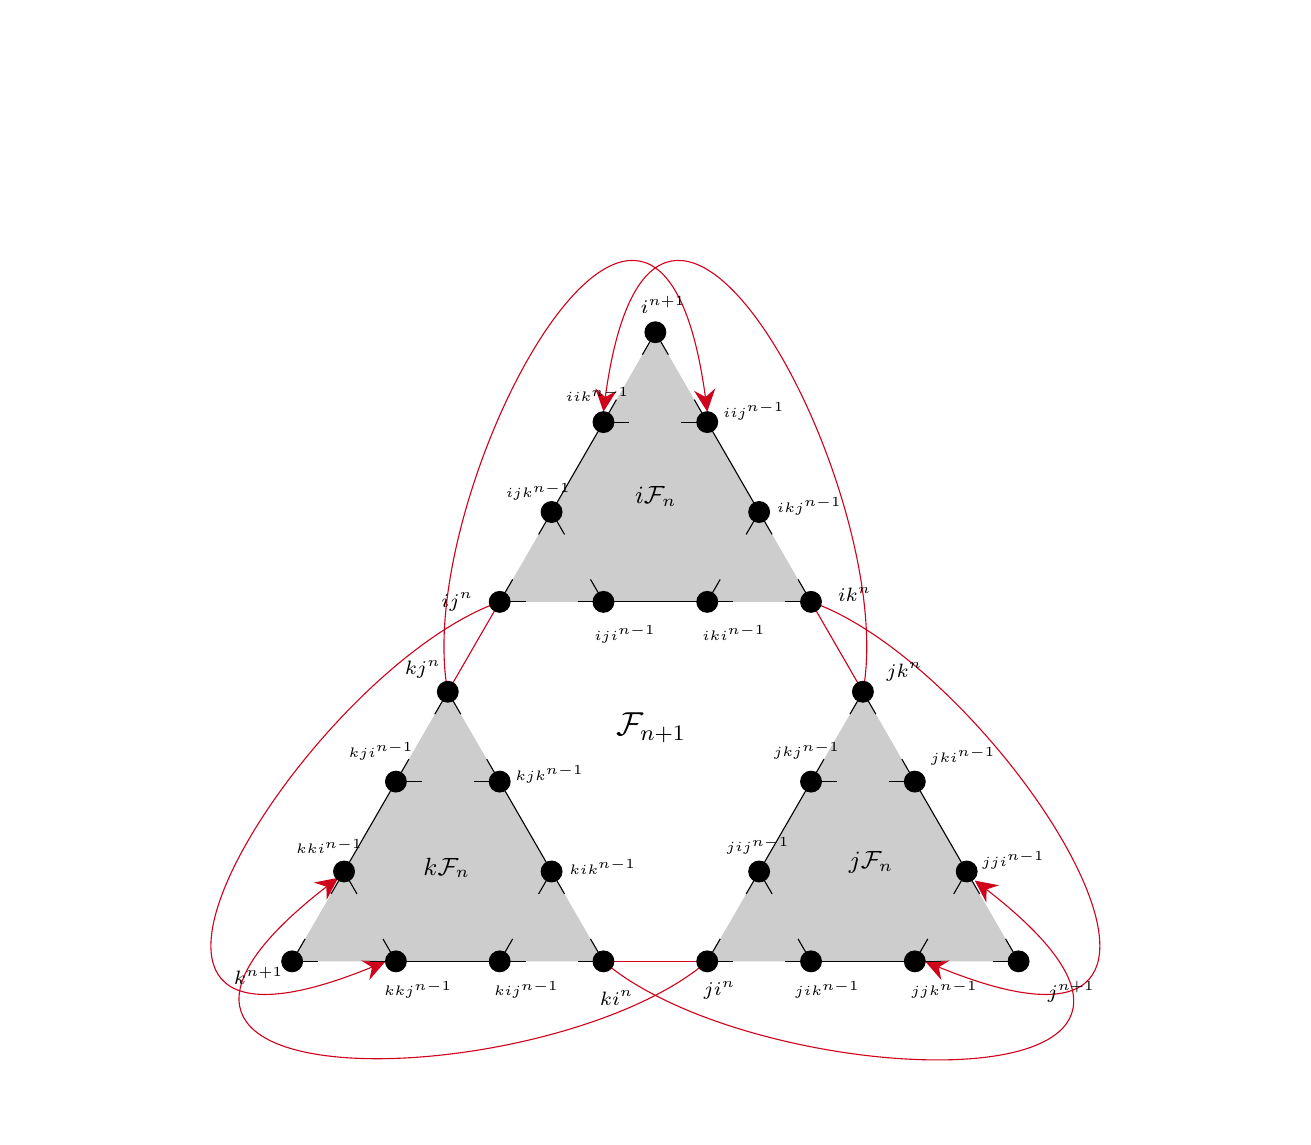
\begin{tikzpicture}[x=0.75pt,y=0.75pt,yscale=-1,xscale=1]
%uncomment if require: \path (0,480); %set diagram left start at 0, and has height of 480

%Curve Lines [id:da6340647836743574] 
\draw [color={rgb, 255:red, 208; green, 2; blue, 27 }  ,draw opacity=1 ]   (372.31,73.87) .. controls (348.71,-105.35) and (229.97,119.21) .. (248,214.33) ;
\draw [shift={(373,79.42)}, rotate = 263.41] [fill={rgb, 255:red, 208; green, 2; blue, 27 }  ,fill opacity=1 ][line width=0.08]  [draw opacity=0] (10.72,-5.15) -- (0,0) -- (10.72,5.15) -- (7.12,0) -- cycle    ;
%Curve Lines [id:da627678148243499] 
\draw [color={rgb, 255:red, 208; green, 2; blue, 27 }  ,draw opacity=1 ]   (212.85,346.42) .. controls (45.85,415.63) and (181.61,202.97) .. (273,171.03) ;
\draw [shift={(218,344.23)}, rotate = 156.59] [fill={rgb, 255:red, 208; green, 2; blue, 27 }  ,fill opacity=1 ][line width=0.08]  [draw opacity=0] (10.72,-5.15) -- (0,0) -- (10.72,5.15) -- (7.12,0) -- cycle    ;
%Straight Lines [id:da09767133400539851] 
\draw [color={rgb, 255:red, 208; green, 2; blue, 27 }  ,draw opacity=1 ][fill={rgb, 255:red, 0; green, 0; blue, 0 }  ,fill opacity=1 ]   (423,171.03) -- (448,214.33) ;
%Curve Lines [id:da22943953288301056] 
\draw [color={rgb, 255:red, 208; green, 2; blue, 27 }  ,draw opacity=1 ]   (323.69,73.87) .. controls (347.29,-105.35) and (466.03,119.21) .. (448,214.33) ;
\draw [shift={(323,79.42)}, rotate = 276.59] [fill={rgb, 255:red, 208; green, 2; blue, 27 }  ,fill opacity=1 ][line width=0.08]  [draw opacity=0] (10.72,-5.15) -- (0,0) -- (10.72,5.15) -- (7.12,0) -- cycle    ;
%Curve Lines [id:da9058564619341327] 
\draw [color={rgb, 255:red, 208; green, 2; blue, 27 }  ,draw opacity=1 ]   (483.15,346.42) .. controls (650.15,415.63) and (514.39,202.97) .. (423,171.03) ;
\draw [shift={(478,344.23)}, rotate = 23.41] [fill={rgb, 255:red, 208; green, 2; blue, 27 }  ,fill opacity=1 ][line width=0.08]  [draw opacity=0] (10.72,-5.15) -- (0,0) -- (10.72,5.15) -- (7.12,0) -- cycle    ;
%Curve Lines [id:da9275343965786502] 
\draw [color={rgb, 255:red, 208; green, 2; blue, 27 }  ,draw opacity=1 ]   (506.35,308.68) .. controls (649.76,418.7) and (396.36,407.4) .. (323,344.23) ;
\draw [shift={(501.88,305.31)}, rotate = 36.59] [fill={rgb, 255:red, 208; green, 2; blue, 27 }  ,fill opacity=1 ][line width=0.08]  [draw opacity=0] (10.72,-5.15) -- (0,0) -- (10.72,5.15) -- (7.12,0) -- cycle    ;
%Curve Lines [id:da5165086732679951] 
\draw [color={rgb, 255:red, 208; green, 2; blue, 27 }  ,draw opacity=1 ]   (190.74,307.35) .. controls (47.31,417.39) and (299.64,407.4) .. (373,344.23) ;
\draw [shift={(195.21,303.98)}, rotate = 143.41] [fill={rgb, 255:red, 208; green, 2; blue, 27 }  ,fill opacity=1 ][line width=0.08]  [draw opacity=0] (10.72,-5.15) -- (0,0) -- (10.72,5.15) -- (7.12,0) -- cycle    ;
%Straight Lines [id:da4908172483439208] 
\draw [draw opacity=0][fill={rgb, 255:red, 155; green, 155; blue, 155 }  ,fill opacity=0.5 ]   (348,41.12) -- (423,171.03) -- (273,171.03) -- (348,41.12) ;
%Straight Lines [id:da8251688389341136] 
\draw [color={rgb, 255:red, 0; green, 0; blue, 0 }  ,draw opacity=1 ]   (323,84.42) -- (298,127.73) ;
%Straight Lines [id:da950543447308454] 
\draw [color={rgb, 255:red, 0; green, 0; blue, 0 }  ,draw opacity=1 ]   (373,84.42) -- (398,127.73) ;
%Straight Lines [id:da2386441368131167] 
\draw [draw opacity=0][fill={rgb, 255:red, 155; green, 155; blue, 155 }  ,fill opacity=0.5 ]   (248,214.33) -- (323,344.23) -- (173,344.23) -- cycle ;
%Straight Lines [id:da5709734393352552] 
\draw [draw opacity=0][fill={rgb, 255:red, 155; green, 155; blue, 155 }  ,fill opacity=0.5 ]   (448,214.33) -- (523,344.23) -- (373,344.23) -- (448,214.33) ;
%Straight Lines [id:da013859710045838192] 
\draw [color={rgb, 255:red, 208; green, 2; blue, 27 }  ,draw opacity=1 ]   (273,171.03) -- (248,214.33) ;
%Straight Lines [id:da40904670312732994] 
\draw [color={rgb, 255:red, 208; green, 2; blue, 27 }  ,draw opacity=1 ]   (323,344.23) -- (373,344.23) ;
%Shape: Circle [id:dp09419565352932491] 
\draw  [color={rgb, 255:red, 0; green, 0; blue, 0 }  ,draw opacity=1 ][fill={rgb, 255:red, 0; green, 0; blue, 0 }  ,fill opacity=1 ] (343,41.12) .. controls (343,38.36) and (345.24,36.12) .. (348,36.12) .. controls (350.76,36.12) and (353,38.36) .. (353,41.12) .. controls (353,43.88) and (350.76,46.12) .. (348,46.12) .. controls (345.24,46.12) and (343,43.88) .. (343,41.12) -- cycle ;
%Shape: Circle [id:dp5410302850263062] 
\draw  [color={rgb, 255:red, 0; green, 0; blue, 0 }  ,draw opacity=1 ][fill={rgb, 255:red, 0; green, 0; blue, 0 }  ,fill opacity=1 ] (318,84.42) .. controls (318,81.66) and (320.24,79.42) .. (323,79.42) .. controls (325.76,79.42) and (328,81.66) .. (328,84.42) .. controls (328,87.19) and (325.76,89.42) .. (323,89.42) .. controls (320.24,89.42) and (318,87.19) .. (318,84.42) -- cycle ;
%Shape: Circle [id:dp7461211893756006] 
\draw  [color={rgb, 255:red, 0; green, 0; blue, 0 }  ,draw opacity=1 ][fill={rgb, 255:red, 0; green, 0; blue, 0 }  ,fill opacity=1 ] (368,84.42) .. controls (368,81.66) and (370.24,79.42) .. (373,79.42) .. controls (375.76,79.42) and (378,81.66) .. (378,84.42) .. controls (378,87.19) and (375.76,89.42) .. (373,89.42) .. controls (370.24,89.42) and (368,87.19) .. (368,84.42) -- cycle ;
%Straight Lines [id:da5924796621213488] 
\draw [color={rgb, 255:red, 0; green, 0; blue, 0 }  ,draw opacity=1 ]   (416.75,160.2) -- (423,171.03) ;
%Straight Lines [id:da9045059453361897] 
\draw [color={rgb, 255:red, 0; green, 0; blue, 0 }  ,draw opacity=1 ]   (323,171.03) -- (373,171.03) ;
%Shape: Circle [id:dp1525072265276488] 
\draw  [color={rgb, 255:red, 0; green, 0; blue, 0 }  ,draw opacity=1 ][fill={rgb, 255:red, 0; green, 0; blue, 0 }  ,fill opacity=1 ] (418,171.03) .. controls (418,168.27) and (420.24,166.03) .. (423,166.03) .. controls (425.76,166.03) and (428,168.27) .. (428,171.03) .. controls (428,173.79) and (425.76,176.03) .. (423,176.03) .. controls (420.24,176.03) and (418,173.79) .. (418,171.03) -- cycle ;
%Shape: Circle [id:dp047393536498240074] 
\draw  [color={rgb, 255:red, 0; green, 0; blue, 0 }  ,draw opacity=1 ][fill={rgb, 255:red, 0; green, 0; blue, 0 }  ,fill opacity=1 ] (368,171.03) .. controls (368,168.27) and (370.24,166.03) .. (373,166.03) .. controls (375.76,166.03) and (378,168.27) .. (378,171.03) .. controls (378,173.79) and (375.76,176.03) .. (373,176.03) .. controls (370.24,176.03) and (368,173.79) .. (368,171.03) -- cycle ;
%Shape: Circle [id:dp6667148477982581] 
\draw  [color={rgb, 255:red, 0; green, 0; blue, 0 }  ,draw opacity=1 ][fill={rgb, 255:red, 0; green, 0; blue, 0 }  ,fill opacity=1 ] (393,127.73) .. controls (393,124.96) and (395.24,122.73) .. (398,122.73) .. controls (400.76,122.73) and (403,124.96) .. (403,127.73) .. controls (403,130.49) and (400.76,132.73) .. (398,132.73) .. controls (395.24,132.73) and (393,130.49) .. (393,127.73) -- cycle ;
%Shape: Circle [id:dp0930047860662353] 
\draw  [color={rgb, 255:red, 0; green, 0; blue, 0 }  ,draw opacity=1 ][fill={rgb, 255:red, 0; green, 0; blue, 0 }  ,fill opacity=1 ] (318,171.03) .. controls (318,168.27) and (320.24,166.03) .. (323,166.03) .. controls (325.76,166.03) and (328,168.27) .. (328,171.03) .. controls (328,173.79) and (325.76,176.03) .. (323,176.03) .. controls (320.24,176.03) and (318,173.79) .. (318,171.03) -- cycle ;
%Shape: Circle [id:dp499697537420682] 
\draw  [color={rgb, 255:red, 0; green, 0; blue, 0 }  ,draw opacity=1 ][fill={rgb, 255:red, 0; green, 0; blue, 0 }  ,fill opacity=1 ] (268,171.03) .. controls (268,168.27) and (270.24,166.03) .. (273,166.03) .. controls (275.76,166.03) and (278,168.27) .. (278,171.03) .. controls (278,173.79) and (275.76,176.03) .. (273,176.03) .. controls (270.24,176.03) and (268,173.79) .. (268,171.03) -- cycle ;
%Shape: Circle [id:dp10015993636469056] 
\draw  [color={rgb, 255:red, 0; green, 0; blue, 0 }  ,draw opacity=1 ][fill={rgb, 255:red, 0; green, 0; blue, 0 }  ,fill opacity=1 ] (293,127.73) .. controls (293,124.96) and (295.24,122.73) .. (298,122.73) .. controls (300.76,122.73) and (303,124.96) .. (303,127.73) .. controls (303,130.49) and (300.76,132.73) .. (298,132.73) .. controls (295.24,132.73) and (293,130.49) .. (293,127.73) -- cycle ;
%Straight Lines [id:da1593048938088859] 
\draw [color={rgb, 255:red, 0; green, 0; blue, 0 }  ,draw opacity=1 ]   (423,257.63) -- (398,300.93) ;
%Straight Lines [id:da2046482586591536] 
\draw [color={rgb, 255:red, 0; green, 0; blue, 0 }  ,draw opacity=1 ]   (273,257.63) -- (298,300.93) ;
%Straight Lines [id:da8020738149050104] 
\draw [color={rgb, 255:red, 0; green, 0; blue, 0 }  ,draw opacity=1 ]   (473,257.63) -- (498,300.93) ;
%Straight Lines [id:da8391950353441284] 
\draw [color={rgb, 255:red, 0; green, 0; blue, 0 }  ,draw opacity=1 ]   (223,257.63) -- (198,300.93) ;
%Straight Lines [id:da9300320099998194] 
\draw [color={rgb, 255:red, 0; green, 0; blue, 0 }  ,draw opacity=1 ]   (223,344.23) -- (273,344.23) ;
%Straight Lines [id:da4907710875283966] 
\draw [color={rgb, 255:red, 0; green, 0; blue, 0 }  ,draw opacity=1 ]   (423,344.23) -- (473,344.23) ;
%Shape: Circle [id:dp772410552034245] 
\draw  [color={rgb, 255:red, 0; green, 0; blue, 0 }  ,draw opacity=1 ][fill={rgb, 255:red, 0; green, 0; blue, 0 }  ,fill opacity=1 ] (443,214.33) .. controls (443,211.57) and (445.24,209.33) .. (448,209.33) .. controls (450.76,209.33) and (453,211.57) .. (453,214.33) .. controls (453,217.09) and (450.76,219.33) .. (448,219.33) .. controls (445.24,219.33) and (443,217.09) .. (443,214.33) -- cycle ;
%Shape: Circle [id:dp13791329940712527] 
\draw  [color={rgb, 255:red, 0; green, 0; blue, 0 }  ,draw opacity=1 ][fill={rgb, 255:red, 0; green, 0; blue, 0 }  ,fill opacity=1 ] (468,257.63) .. controls (468,254.87) and (470.24,252.63) .. (473,252.63) .. controls (475.76,252.63) and (478,254.87) .. (478,257.63) .. controls (478,260.39) and (475.76,262.63) .. (473,262.63) .. controls (470.24,262.63) and (468,260.39) .. (468,257.63) -- cycle ;
%Shape: Circle [id:dp966990717450676] 
\draw  [color={rgb, 255:red, 0; green, 0; blue, 0 }  ,draw opacity=1 ][fill={rgb, 255:red, 0; green, 0; blue, 0 }  ,fill opacity=1 ] (493,300.93) .. controls (493,298.17) and (495.24,295.93) .. (498,295.93) .. controls (500.76,295.93) and (503,298.17) .. (503,300.93) .. controls (503,303.69) and (500.76,305.93) .. (498,305.93) .. controls (495.24,305.93) and (493,303.69) .. (493,300.93) -- cycle ;
%Shape: Circle [id:dp8748838953814821] 
\draw  [color={rgb, 255:red, 0; green, 0; blue, 0 }  ,draw opacity=1 ][fill={rgb, 255:red, 0; green, 0; blue, 0 }  ,fill opacity=1 ] (518,344.23) .. controls (518,341.47) and (520.24,339.23) .. (523,339.23) .. controls (525.76,339.23) and (528,341.47) .. (528,344.23) .. controls (528,346.99) and (525.76,349.23) .. (523,349.23) .. controls (520.24,349.23) and (518,346.99) .. (518,344.23) -- cycle ;
%Shape: Circle [id:dp6114202388322192] 
\draw  [color={rgb, 255:red, 0; green, 0; blue, 0 }  ,draw opacity=1 ][fill={rgb, 255:red, 0; green, 0; blue, 0 }  ,fill opacity=1 ] (468,344.23) .. controls (468,341.47) and (470.24,339.23) .. (473,339.23) .. controls (475.76,339.23) and (478,341.47) .. (478,344.23) .. controls (478,346.99) and (475.76,349.23) .. (473,349.23) .. controls (470.24,349.23) and (468,346.99) .. (468,344.23) -- cycle ;
%Shape: Circle [id:dp3276869135971108] 
\draw  [color={rgb, 255:red, 0; green, 0; blue, 0 }  ,draw opacity=1 ][fill={rgb, 255:red, 0; green, 0; blue, 0 }  ,fill opacity=1 ] (418,344.23) .. controls (418,341.47) and (420.24,339.23) .. (423,339.23) .. controls (425.76,339.23) and (428,341.47) .. (428,344.23) .. controls (428,346.99) and (425.76,349.23) .. (423,349.23) .. controls (420.24,349.23) and (418,346.99) .. (418,344.23) -- cycle ;
%Shape: Circle [id:dp02985749056388065] 
\draw  [color={rgb, 255:red, 0; green, 0; blue, 0 }  ,draw opacity=1 ][fill={rgb, 255:red, 0; green, 0; blue, 0 }  ,fill opacity=1 ] (368,344.23) .. controls (368,341.47) and (370.24,339.23) .. (373,339.23) .. controls (375.76,339.23) and (378,341.47) .. (378,344.23) .. controls (378,346.99) and (375.76,349.23) .. (373,349.23) .. controls (370.24,349.23) and (368,346.99) .. (368,344.23) -- cycle ;
%Shape: Circle [id:dp8089361914056541] 
\draw  [color={rgb, 255:red, 0; green, 0; blue, 0 }  ,draw opacity=1 ][fill={rgb, 255:red, 0; green, 0; blue, 0 }  ,fill opacity=1 ] (393,300.93) .. controls (393,298.17) and (395.24,295.93) .. (398,295.93) .. controls (400.76,295.93) and (403,298.17) .. (403,300.93) .. controls (403,303.69) and (400.76,305.93) .. (398,305.93) .. controls (395.24,305.93) and (393,303.69) .. (393,300.93) -- cycle ;
%Shape: Circle [id:dp9009952759752804] 
\draw  [color={rgb, 255:red, 0; green, 0; blue, 0 }  ,draw opacity=1 ][fill={rgb, 255:red, 0; green, 0; blue, 0 }  ,fill opacity=1 ] (418,257.63) .. controls (418,254.87) and (420.24,252.63) .. (423,252.63) .. controls (425.76,252.63) and (428,254.87) .. (428,257.63) .. controls (428,260.39) and (425.76,262.63) .. (423,262.63) .. controls (420.24,262.63) and (418,260.39) .. (418,257.63) -- cycle ;
%Shape: Circle [id:dp5434259933757828] 
\draw  [color={rgb, 255:red, 0; green, 0; blue, 0 }  ,draw opacity=1 ][fill={rgb, 255:red, 0; green, 0; blue, 0 }  ,fill opacity=1 ] (243,214.33) .. controls (243,211.57) and (245.24,209.33) .. (248,209.33) .. controls (250.76,209.33) and (253,211.57) .. (253,214.33) .. controls (253,217.09) and (250.76,219.33) .. (248,219.33) .. controls (245.24,219.33) and (243,217.09) .. (243,214.33) -- cycle ;
%Shape: Circle [id:dp08426838748162213] 
\draw  [color={rgb, 255:red, 0; green, 0; blue, 0 }  ,draw opacity=1 ][fill={rgb, 255:red, 0; green, 0; blue, 0 }  ,fill opacity=1 ] (268,257.63) .. controls (268,254.87) and (270.24,252.63) .. (273,252.63) .. controls (275.76,252.63) and (278,254.87) .. (278,257.63) .. controls (278,260.39) and (275.76,262.63) .. (273,262.63) .. controls (270.24,262.63) and (268,260.39) .. (268,257.63) -- cycle ;
%Shape: Circle [id:dp22550614513944622] 
\draw  [color={rgb, 255:red, 0; green, 0; blue, 0 }  ,draw opacity=1 ][fill={rgb, 255:red, 0; green, 0; blue, 0 }  ,fill opacity=1 ] (293,300.93) .. controls (293,298.17) and (295.24,295.93) .. (298,295.93) .. controls (300.76,295.93) and (303,298.17) .. (303,300.93) .. controls (303,303.69) and (300.76,305.93) .. (298,305.93) .. controls (295.24,305.93) and (293,303.69) .. (293,300.93) -- cycle ;
%Shape: Circle [id:dp4501401628734605] 
\draw  [color={rgb, 255:red, 0; green, 0; blue, 0 }  ,draw opacity=1 ][fill={rgb, 255:red, 0; green, 0; blue, 0 }  ,fill opacity=1 ] (318,344.23) .. controls (318,341.47) and (320.24,339.23) .. (323,339.23) .. controls (325.76,339.23) and (328,341.47) .. (328,344.23) .. controls (328,346.99) and (325.76,349.23) .. (323,349.23) .. controls (320.24,349.23) and (318,346.99) .. (318,344.23) -- cycle ;
%Shape: Circle [id:dp6206041371213686] 
\draw  [color={rgb, 255:red, 0; green, 0; blue, 0 }  ,draw opacity=1 ][fill={rgb, 255:red, 0; green, 0; blue, 0 }  ,fill opacity=1 ] (268,344.23) .. controls (268,341.47) and (270.24,339.23) .. (273,339.23) .. controls (275.76,339.23) and (278,341.47) .. (278,344.23) .. controls (278,346.99) and (275.76,349.23) .. (273,349.23) .. controls (270.24,349.23) and (268,346.99) .. (268,344.23) -- cycle ;
%Shape: Circle [id:dp5151666915081357] 
\draw  [color={rgb, 255:red, 0; green, 0; blue, 0 }  ,draw opacity=1 ][fill={rgb, 255:red, 0; green, 0; blue, 0 }  ,fill opacity=1 ] (218,344.23) .. controls (218,341.47) and (220.24,339.23) .. (223,339.23) .. controls (225.76,339.23) and (228,341.47) .. (228,344.23) .. controls (228,346.99) and (225.76,349.23) .. (223,349.23) .. controls (220.24,349.23) and (218,346.99) .. (218,344.23) -- cycle ;
%Shape: Circle [id:dp9385107669444044] 
\draw  [color={rgb, 255:red, 0; green, 0; blue, 0 }  ,draw opacity=1 ][fill={rgb, 255:red, 0; green, 0; blue, 0 }  ,fill opacity=1 ] (168,344.23) .. controls (168,341.47) and (170.24,339.23) .. (173,339.23) .. controls (175.76,339.23) and (178,341.47) .. (178,344.23) .. controls (178,346.99) and (175.76,349.23) .. (173,349.23) .. controls (170.24,349.23) and (168,346.99) .. (168,344.23) -- cycle ;
%Shape: Circle [id:dp24812177389522416] 
\draw  [color={rgb, 255:red, 0; green, 0; blue, 0 }  ,draw opacity=1 ][fill={rgb, 255:red, 0; green, 0; blue, 0 }  ,fill opacity=1 ] (193,300.93) .. controls (193,298.17) and (195.24,295.93) .. (198,295.93) .. controls (200.76,295.93) and (203,298.17) .. (203,300.93) .. controls (203,303.69) and (200.76,305.93) .. (198,305.93) .. controls (195.24,305.93) and (193,303.69) .. (193,300.93) -- cycle ;
%Shape: Circle [id:dp8826858020347639] 
\draw  [color={rgb, 255:red, 0; green, 0; blue, 0 }  ,draw opacity=1 ][fill={rgb, 255:red, 0; green, 0; blue, 0 }  ,fill opacity=1 ] (218,257.63) .. controls (218,254.87) and (220.24,252.63) .. (223,252.63) .. controls (225.76,252.63) and (228,254.87) .. (228,257.63) .. controls (228,260.39) and (225.76,262.63) .. (223,262.63) .. controls (220.24,262.63) and (218,260.39) .. (218,257.63) -- cycle ;
%Straight Lines [id:da8776269251813866] 
\draw [color={rgb, 255:red, 0; green, 0; blue, 0 }  ,draw opacity=1 ]   (398,127.73) -- (404.25,138.55) ;
%Straight Lines [id:da9955549237915113] 
\draw [color={rgb, 255:red, 0; green, 0; blue, 0 }  ,draw opacity=1 ]   (373,171.03) -- (385.5,171.03) ;
%Straight Lines [id:da4488270788403692] 
\draw [color={rgb, 255:red, 0; green, 0; blue, 0 }  ,draw opacity=1 ]   (373,171.03) -- (379.25,160.2) ;
%Straight Lines [id:da1308264347161019] 
\draw [color={rgb, 255:red, 0; green, 0; blue, 0 }  ,draw opacity=1 ]   (391.75,138.55) -- (398,127.73) ;
%Straight Lines [id:da8147425069644019] 
\draw [color={rgb, 255:red, 0; green, 0; blue, 0 }  ,draw opacity=1 ]   (310.5,171.03) -- (323,171.03) ;
%Straight Lines [id:da6960348206340405] 
\draw [color={rgb, 255:red, 0; green, 0; blue, 0 }  ,draw opacity=1 ]   (273,171.03) -- (285.5,171.03) ;
%Straight Lines [id:da6459325290748372] 
\draw [color={rgb, 255:red, 0; green, 0; blue, 0 }  ,draw opacity=1 ]   (273,171.03) -- (279.25,160.2) ;
%Straight Lines [id:da8580035925016816] 
\draw [color={rgb, 255:red, 0; green, 0; blue, 0 }  ,draw opacity=1 ]   (291.75,138.55) -- (298,127.73) ;
%Straight Lines [id:da8455841124628454] 
\draw [color={rgb, 255:red, 0; green, 0; blue, 0 }  ,draw opacity=1 ]   (298,127.73) -- (304.25,138.55) ;
%Straight Lines [id:da554164475767863] 
\draw [color={rgb, 255:red, 0; green, 0; blue, 0 }  ,draw opacity=1 ]   (316.75,160.2) -- (323,171.03) ;
%Straight Lines [id:da5006626646769308] 
\draw [color={rgb, 255:red, 0; green, 0; blue, 0 }  ,draw opacity=1 ]   (323,84.42) -- (335.5,84.42) ;
%Straight Lines [id:da8881224313175813] 
\draw [color={rgb, 255:red, 0; green, 0; blue, 0 }  ,draw opacity=1 ]   (360.5,84.42) -- (373,84.42) ;
%Straight Lines [id:da7527962493620683] 
\draw [color={rgb, 255:red, 0; green, 0; blue, 0 }  ,draw opacity=1 ]   (348,41.12) -- (354.25,51.95) ;
%Straight Lines [id:da5475099905255547] 
\draw [color={rgb, 255:red, 0; green, 0; blue, 0 }  ,draw opacity=1 ]   (341.75,51.95) -- (348,41.12) ;
%Straight Lines [id:da4539454247192083] 
\draw [color={rgb, 255:red, 0; green, 0; blue, 0 }  ,draw opacity=1 ]   (410.5,171.03) -- (423,171.03) ;
%Straight Lines [id:da6038644772688284] 
\draw [color={rgb, 255:red, 0; green, 0; blue, 0 }  ,draw opacity=1 ]   (366.75,73.6) -- (373,84.42) ;
%Straight Lines [id:da3421709207976611] 
\draw [color={rgb, 255:red, 0; green, 0; blue, 0 }  ,draw opacity=1 ]   (323,84.42) -- (329.25,73.6) ;
%Straight Lines [id:da4963105553761995] 
\draw [color={rgb, 255:red, 0; green, 0; blue, 0 }  ,draw opacity=1 ]   (448,214.33) -- (454.25,225.15) ;
%Straight Lines [id:da48179368104404485] 
\draw [color={rgb, 255:red, 0; green, 0; blue, 0 }  ,draw opacity=1 ]   (441.75,225.15) -- (448,214.33) ;
%Straight Lines [id:da7513923365692994] 
\draw [color={rgb, 255:red, 0; green, 0; blue, 0 }  ,draw opacity=1 ]   (466.75,246.8) -- (473,257.63) ;
%Straight Lines [id:da40748772926721144] 
\draw [color={rgb, 255:red, 0; green, 0; blue, 0 }  ,draw opacity=1 ]   (423,257.63) -- (429.25,246.8) ;
%Straight Lines [id:da7089704931599781] 
\draw [color={rgb, 255:red, 0; green, 0; blue, 0 }  ,draw opacity=1 ]   (498,300.93) -- (504.25,311.76) ;
%Straight Lines [id:da8668786649669828] 
\draw [color={rgb, 255:red, 0; green, 0; blue, 0 }  ,draw opacity=1 ]   (491.75,311.76) -- (498,300.93) ;
%Straight Lines [id:da10174625487874134] 
\draw [color={rgb, 255:red, 0; green, 0; blue, 0 }  ,draw opacity=1 ]   (398,300.93) -- (404.25,311.76) ;
%Straight Lines [id:da8688575148314166] 
\draw [color={rgb, 255:red, 0; green, 0; blue, 0 }  ,draw opacity=1 ]   (391.75,311.76) -- (398,300.93) ;
%Straight Lines [id:da9721442743892272] 
\draw [color={rgb, 255:red, 0; green, 0; blue, 0 }  ,draw opacity=1 ]   (316.75,333.41) -- (323,344.23) ;
%Straight Lines [id:da6452240364714339] 
\draw [color={rgb, 255:red, 0; green, 0; blue, 0 }  ,draw opacity=1 ]   (273,344.23) -- (279.25,333.41) ;
%Straight Lines [id:da41038324916345736] 
\draw [color={rgb, 255:red, 0; green, 0; blue, 0 }  ,draw opacity=1 ]   (198,300.93) -- (204.25,311.76) ;
%Straight Lines [id:da12621377987018945] 
\draw [color={rgb, 255:red, 0; green, 0; blue, 0 }  ,draw opacity=1 ]   (191.75,311.76) -- (198,300.93) ;
%Straight Lines [id:da9669042521969002] 
\draw [color={rgb, 255:red, 0; green, 0; blue, 0 }  ,draw opacity=1 ]   (248,214.33) -- (254.25,225.15) ;
%Straight Lines [id:da04125569634074644] 
\draw [color={rgb, 255:red, 0; green, 0; blue, 0 }  ,draw opacity=1 ]   (241.75,225.15) -- (248,214.33) ;
%Straight Lines [id:da0608711180356325] 
\draw [color={rgb, 255:red, 0; green, 0; blue, 0 }  ,draw opacity=1 ]   (516.75,333.41) -- (523,344.23) ;
%Straight Lines [id:da0037529496174986132] 
\draw [color={rgb, 255:red, 0; green, 0; blue, 0 }  ,draw opacity=1 ]   (473,344.23) -- (479.25,333.41) ;
%Straight Lines [id:da03248429633123573] 
\draw [color={rgb, 255:red, 0; green, 0; blue, 0 }  ,draw opacity=1 ]   (416.75,333.41) -- (423,344.23) ;
%Straight Lines [id:da5148662977941516] 
\draw [color={rgb, 255:red, 0; green, 0; blue, 0 }  ,draw opacity=1 ]   (373,344.23) -- (379.25,333.41) ;
%Straight Lines [id:da9306512352228411] 
\draw [color={rgb, 255:red, 0; green, 0; blue, 0 }  ,draw opacity=1 ]   (298,300.93) -- (304.25,311.76) ;
%Straight Lines [id:da027594020068589353] 
\draw [color={rgb, 255:red, 0; green, 0; blue, 0 }  ,draw opacity=1 ]   (291.75,311.76) -- (298,300.93) ;
%Straight Lines [id:da1270812496793432] 
\draw [color={rgb, 255:red, 0; green, 0; blue, 0 }  ,draw opacity=1 ]   (266.75,246.8) -- (273,257.63) ;
%Straight Lines [id:da013147132830545027] 
\draw [color={rgb, 255:red, 0; green, 0; blue, 0 }  ,draw opacity=1 ]   (223,257.63) -- (229.25,246.8) ;
%Straight Lines [id:da04578806852291262] 
\draw [color={rgb, 255:red, 0; green, 0; blue, 0 }  ,draw opacity=1 ]   (216.75,333.41) -- (223,344.23) ;
%Straight Lines [id:da05762470054675628] 
\draw [color={rgb, 255:red, 0; green, 0; blue, 0 }  ,draw opacity=1 ]   (173,344.23) -- (179.25,333.41) ;
%Straight Lines [id:da9736253005816671] 
\draw [color={rgb, 255:red, 0; green, 0; blue, 0 }  ,draw opacity=1 ]   (423,257.63) -- (435.5,257.63) ;
%Straight Lines [id:da8935338348403978] 
\draw [color={rgb, 255:red, 0; green, 0; blue, 0 }  ,draw opacity=1 ]   (460.5,257.63) -- (473,257.63) ;
%Straight Lines [id:da8693837835721938] 
\draw [color={rgb, 255:red, 0; green, 0; blue, 0 }  ,draw opacity=1 ]   (410.5,344.23) -- (423,344.23) ;
%Straight Lines [id:da18026221733631065] 
\draw [color={rgb, 255:red, 0; green, 0; blue, 0 }  ,draw opacity=1 ]   (373,344.23) -- (385.5,344.23) ;
%Straight Lines [id:da738518512643519] 
\draw [color={rgb, 255:red, 0; green, 0; blue, 0 }  ,draw opacity=1 ]   (510.5,344.23) -- (523,344.23) ;
%Straight Lines [id:da10499710300695209] 
\draw [color={rgb, 255:red, 0; green, 0; blue, 0 }  ,draw opacity=1 ]   (473,344.23) -- (485.5,344.23) ;
%Straight Lines [id:da4487074414222847] 
\draw [color={rgb, 255:red, 0; green, 0; blue, 0 }  ,draw opacity=1 ]   (273,344.23) -- (285.5,344.23) ;
%Straight Lines [id:da3396865421872004] 
\draw [color={rgb, 255:red, 0; green, 0; blue, 0 }  ,draw opacity=1 ]   (310.5,344.23) -- (323,344.23) ;
%Straight Lines [id:da589027845710651] 
\draw [color={rgb, 255:red, 0; green, 0; blue, 0 }  ,draw opacity=1 ]   (210.5,344.23) -- (223,344.23) ;
%Straight Lines [id:da3286282513866896] 
\draw [color={rgb, 255:red, 0; green, 0; blue, 0 }  ,draw opacity=1 ]   (173,344.23) -- (185.5,344.23) ;
%Straight Lines [id:da02329621050126196] 
\draw [color={rgb, 255:red, 0; green, 0; blue, 0 }  ,draw opacity=1 ]   (260.5,257.63) -- (273,257.63) ;
%Straight Lines [id:da4466574357616795] 
\draw [color={rgb, 255:red, 0; green, 0; blue, 0 }  ,draw opacity=1 ]   (223,257.63) -- (235.5,257.63) ;

% Text Node
\draw (379.33,73.82) node [anchor=north west][inner sep=0.75pt]  [font=\tiny,color={rgb, 255:red, 0; green, 0; blue, 0 }  ,opacity=1 ]  {$iij^{n-1}$};
% Text Node
\draw (303.67,66.16) node [anchor=north west][inner sep=0.75pt]  [font=\tiny]  {$iik^{n-1}$};
% Text Node
\draw (369.33,181.09) node [anchor=north west][inner sep=0.75pt]  [font=\tiny]  {$iki^{n-1}$};
% Text Node
\draw (405.33,119.49) node [anchor=north west][inner sep=0.75pt]  [font=\tiny]  {$ikj^{n-1}$};
% Text Node
\draw (317.33,181.09) node [anchor=north west][inner sep=0.75pt]  [font=\tiny]  {$iji^{n-1}$};
% Text Node
\draw (274.67,112.49) node [anchor=north west][inner sep=0.75pt]  [font=\tiny]  {$ijk^{n-1}$};
% Text Node
\draw (339.67,22.49) node [anchor=north west][inner sep=0.75pt]  [font=\scriptsize]  {$i^{n+1}$};
% Text Node
\draw (479.33,239.95) node [anchor=north west][inner sep=0.75pt]  [font=\tiny]  {$jki^{n-1}$};
% Text Node
\draw (504,289.95) node [anchor=north west][inner sep=0.75pt]  [font=\tiny]  {$jji^{n-1}$};
% Text Node
\draw (403.67,237.28) node [anchor=north west][inner sep=0.75pt]  [font=\tiny]  {$jkj^{n-1}$};
% Text Node
\draw (381,282.95) node [anchor=north west][inner sep=0.75pt]  [font=\tiny]  {$jij^{n-1}$};
% Text Node
\draw (470,352.49) node [anchor=north west][inner sep=0.75pt]  [font=\tiny]  {$jjk^{n-1}$};
% Text Node
\draw (414,352.49) node [anchor=north west][inner sep=0.75pt]  [font=\tiny]  {$jik^{n-1}$};
% Text Node
\draw (269,352.49) node [anchor=north west][inner sep=0.75pt]  [font=\tiny]  {$kij^{n-1}$};
% Text Node
\draw (216,352.49) node [anchor=north west][inner sep=0.75pt]  [font=\tiny]  {$kkj^{n-1}$};
% Text Node
\draw (173.67,283.95) node [anchor=north west][inner sep=0.75pt]  [font=\tiny]  {$kki^{n-1}$};
% Text Node
\draw (305.33,293.95) node [anchor=north west][inner sep=0.75pt]  [font=\tiny]  {$kik^{n-1}$};
% Text Node
\draw (199,237.61) node [anchor=north west][inner sep=0.75pt]  [font=\tiny]  {$kji^{n-1}$};
% Text Node
\draw (279.33,248.61) node [anchor=north west][inner sep=0.75pt]  [font=\tiny]  {$kjk^{n-1}$};
% Text Node
\draw (434.67,162.82) node [anchor=north west][inner sep=0.75pt]  [font=\scriptsize]  {$ik^{n}$};
% Text Node
\draw (243.67,165.49) node [anchor=north west][inner sep=0.75pt]  [font=\scriptsize]  {$ij^{n}$};
% Text Node
\draw (226,197.82) node [anchor=north west][inner sep=0.75pt]  [font=\scriptsize]  {$kj^{n}$};
% Text Node
\draw (458,199.16) node [anchor=north west][inner sep=0.75pt]  [font=\scriptsize]  {$jk^{n}$};
% Text Node
\draw (535.67,352.49) node [anchor=north west][inner sep=0.75pt]  [font=\scriptsize]  {$j^{n+1}$};
% Text Node
\draw (143.67,345.82) node [anchor=north west][inner sep=0.75pt]  [font=\scriptsize]  {$k^{n+1}$};
% Text Node
\draw (320,357.16) node [anchor=north west][inner sep=0.75pt]  [font=\scriptsize]  {$ki^{n}$};
% Text Node
\draw (370,352.49) node [anchor=north west][inner sep=0.75pt]  [font=\scriptsize,color={rgb, 255:red, 0; green, 0; blue, 0 }  ,opacity=1 ]  {$ji^{n}$};
% Text Node
\draw (337,114.07) node [anchor=north west][inner sep=0.75pt]  [font=\small]  {$i\mathcal{F}_{n}$};
% Text Node
\draw (440,290.07) node [anchor=north west][inner sep=0.75pt]  [font=\small]  {$j\mathcal{F}_{n}$};
% Text Node
\draw (235,293.07) node [anchor=north west][inner sep=0.75pt]  [font=\small]  {$k\mathcal{F}_{n}$};
% Text Node
\draw (328,223.07) node [anchor=north west][inner sep=0.75pt]  [font=\large]  {$\mathcal{F}_{n+1}$};


\end{tikzpicture}
    \caption{Recursive structure of Fibonacci-Tower graphs}
    \label{fig:recurssive_fibonacci_graph}
\end{figure}

The formal recursive definition of the arc sets of the Fibonacci-Tower graphs $\mathcal{F}_{n+1}$, for $n\geq 1$, is

\begin{equation}\label{eq:arc_set_recurssive}
\begin{split}
    A(\mathcal{F}_{n+1})=&\left\{(ir,is)\mid i\neq j \in T, (ir,is)\in A(\mathcal{F}_{n})    \right\} \\ 
    \cup& \left\{(ik^{n},ik^{n})\mid i\neq j \in T, k=6-i-j    \right\} \\
    \cup& \left\{(ik^{n},jjk^{n-1})\mid i\neq j \in T, k=6-i-j    \right\}, 
\end{split}
\end{equation}

that is a union of three sets, in which the first,   corresponds to the arcs associated with moves of discs $d<n+1$, the second corresponds to the arcs associated with the classical moves of the largest disc, and the third corresponds to the arcs associated to the Magic moves of the largest disc.


As is the case for Hanoi graphs, many properties of Fibonacci-Tower graphs can be deduced from their recursive structure. In the next lines of this section, we consider some properties of the graph $\mathcal{F}_{n}$ and its underlying undirected graph\footnote{The underlying undirected graph of a directed graph is one with the same set of vertices, but a different set of edges. In particular, between any pair of vertices $x$ and $y$, if the directed graph has an arc $(x,y)$ or an arc $(y,x)$, the underlying undirected graph includes an edge $\{x, y\}$.} denoted by $\bm{\mathcal{F}_{n}}$.

 





\begin{theorem}
    For all integers $n\geq 2$, we have 
    \begin{equation}
        |B_{n}|=3|B_{n-1}|+6,
    \end{equation}
    where $|B_{0}|=0$.
\end{theorem}
\begin{proof}
According to \eqref{eq:arc_set_recurssive}, $\mathcal{F}_{n}$ is composed of three copies of $\mathcal{F}_{n-1}$ each has $|B_{n-1}|$ arc that corresponds to a Magic move of discs $d<n$, in addition to $6$ arcs of Magic moves related the largest disc $n$. 


    % The case $n=0$ is trivial, as well as the case $n=1$ where no Magic move can be applied. Now let's suppose that the recurrence relation is true up to $k<n$. The graph $\mathcal{F}_{n}$ is constructed of three copies of $F_{n-1}$, in addition to the arcs corresponds to Magic moves of the largest disc $n$. The number of the latter arcs is exactly $6$, since the only states in which a Magic move can be applied to the largest disc are those where the largest disc is stacked onto one peg ($3$ possibilities), and the subtower of the first $n-1$ disc is stacked onto another peg ($2$ possibilities). Therefore, $u_{n}=3u_{n-1}+6$. 
\end{proof}

\begin{corollary}
    For all integers $n\geq 1$, we have 
    \begin{equation}
        |B_{n}|=3^{n}-3.
    \end{equation}
\end{corollary}


According to \eqref{eq_arc_set_union}, the number of arcs in $\mathcal{F}_{n}$ satisfies
\begin{equation}
     |A(\mathcal{F}_{n})|=|\mathcal{H}_{n}|+|B_{n}|.
\end{equation}

Knowing that the number of arcs in the directed classical Hanoi graph $\mathcal{H}_{n}$ is $3(3^{n}-1)$ \cite[Proposition 5.43]{hinz2018tower}, a definitive formula of $|A(\mathcal{F}_{n})|$ can be deduced.

\begin{corollary}
    For all integers $n\geq 1$, we have 
    \begin{equation}
    |A(\mathcal{F}_{n})|=4\cdot3^{n}-6.
\end{equation}
\end{corollary}

The number of arcs in $\mathcal{F}_{n}$ satisfies also the following recursive formula. 

\begin{proposition}
    For all integers $n\geq 1$, we have 
    \begin{equation}
    |A(\mathcal{F}_{n})|=3|A(\mathcal{F}_{n-1})|+12.
\end{equation}
\end{proposition}
\begin{proof}
    Using Relation \eqref{eq:arc_set_recurssive}.
\end{proof}












The number of arcs in $\bm{\mathcal{F}_{n}}$ can be deduced using the same reasoning as it is the case for $\mathcal{F}_{n}$.

 


\begin{proposition}
    For all integers $n\geq 1$, we have 
    \begin{equation}
    |A(\bm{\mathcal{F}_{n}})|=\dfrac{1}{2}\left(5\cdot3^{n}-9\right).
\end{equation}
\end{proposition}

\begin{proposition}
    For all integers $n\geq 2$, we have 
    \begin{equation}
    |A(\bm{\mathcal{F}_{n}})|=3|A(\mathcal{F}_{n-1})|+9,
\end{equation}
where $|A(\bm{\mathcal{F}_{1}})|=3$.
\end{proposition}


\begin{table}[H]
\centering
\begin{tabular}{@{}lllllllllll@{}}
\toprule
$n$       & 0 & 1 & 2 & 3  & 4  & 5  & 6   & 7   & 8   & $\cdots$ \\ \midrule
$|A(\mathcal{F}_{n})|$   & 0 & 6& 30& 102& 318& 966& 2910& 8742& 26238&  $\cdots$ \\ \midrule
$|A(\bm{\mathcal{F}_{n}})|$   & 0 & 3& 18& 63& 198& 603& 1818& 5463& 16398&  $\cdots$ \\
 \bottomrule
\end{tabular}
\caption{First values of $|A(\mathcal{F}_{n})|$ and $|A(\bm{\mathcal{F}_{n}})|$}
\end{table}


\begin{theorem}\label{theorem_fibonacci_not_planar}
    For all integers  $n\geq 2$, the graph $\bm{\mathcal{F}_{n}}$   is not planar.
\end{theorem}
\begin{proof}
It suffice to prove that $\bm{\mathcal{F}_{2}}$ is not planar, since  $\bm{\mathcal{F}_{n}} \subset \bm{\mathcal{F}_{n+1}}$ for all $n\geq 1$.

We prove now that $K_{3,3}$ is a minor of graph $\bm{\mathcal{F}_{2}}$. Figure \ref{fig:proof_planarity} illustrates this. First construct a subgraph $\mathcal{G}^{1}$ of $\bm{\mathcal{F}_{2}}$ by deleting the dashed edges $\{12,32\}$, $\{23,13\}$, and $\{31,21\}$, and then contract each of the edges (merging the two vertices that the edged connects) $\{12,13\}$, $\{23,21\}$, and $\{31,32\}$ to become the vertices $x$, $y$, and $z$, respectively. Therefore,  the obtained graph $\mathcal{G}^{2}$ can be split into two subsets of vertices, $\{11,22,33\}$ and $\{x,y,z\}$, each of them is stable, and where the set of edges of $\mathcal{G}^{2}$ 
is the set of all possible edges between $\{11,22,33\}$ and $\{x,y,z\}$. Consequently,  $\mathcal{G}^{2}$   is isomorphic to the complete
bipartite graph $K_{3,3}$. Hence, $K_{3,3}$ is a minor of $\bm{\mathcal{F}_{2}}$, which implies that $\bm{\mathcal{F}_{2}}$ is not planar, according to by Wagner’s theorem.

\begin{figure}[H]
    \centering
    

\tikzset{every picture/.style={line width=0.75pt}} %set default line width to 0.75pt        

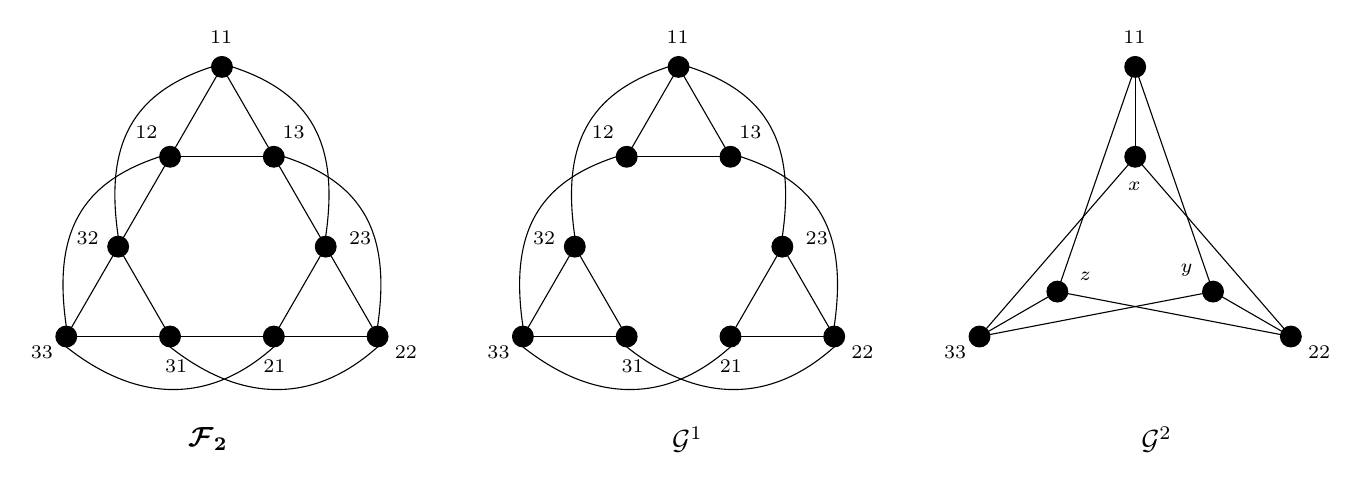
\begin{tikzpicture}[x=0.75pt,y=0.75pt,yscale=-1,xscale=1]
%uncomment if require: \path (0,499); %set diagram left start at 0, and has height of 499

%Straight Lines [id:da43722138337806293] 
\draw [color={rgb, 255:red, 0; green, 0; blue, 0 }  ,draw opacity=1 ]   (69.33,64.33) -- (119.33,64.33) ;
%Straight Lines [id:da2957688143327448] 
\draw [color={rgb, 255:red, 0; green, 0; blue, 0 }  ,draw opacity=1 ]   (94.33,21.03) -- (119.33,64.33) ;
%Straight Lines [id:da8303980756588274] 
\draw [color={rgb, 255:red, 0; green, 0; blue, 0 }  ,draw opacity=1 ]   (94.33,21.03) -- (69.33,64.33) ;
%Shape: Circle [id:dp7257930221652149] 
\draw  [color={rgb, 255:red, 0; green, 0; blue, 0 }  ,draw opacity=1 ][fill={rgb, 255:red, 0; green, 0; blue, 0 }  ,fill opacity=1 ] (89.33,21.03) .. controls (89.33,18.27) and (91.57,16.03) .. (94.33,16.03) .. controls (97.09,16.03) and (99.33,18.27) .. (99.33,21.03) .. controls (99.33,23.79) and (97.09,26.03) .. (94.33,26.03) .. controls (91.57,26.03) and (89.33,23.79) .. (89.33,21.03) -- cycle ;
%Shape: Circle [id:dp1781058612997104] 
\draw  [color={rgb, 255:red, 0; green, 0; blue, 0 }  ,draw opacity=1 ][fill={rgb, 255:red, 0; green, 0; blue, 0 }  ,fill opacity=1 ] (64.33,64.33) .. controls (64.33,61.57) and (66.57,59.33) .. (69.33,59.33) .. controls (72.09,59.33) and (74.33,61.57) .. (74.33,64.33) .. controls (74.33,67.09) and (72.09,69.33) .. (69.33,69.33) .. controls (66.57,69.33) and (64.33,67.09) .. (64.33,64.33) -- cycle ;
%Shape: Circle [id:dp6337213769694507] 
\draw  [color={rgb, 255:red, 0; green, 0; blue, 0 }  ,draw opacity=1 ][fill={rgb, 255:red, 0; green, 0; blue, 0 }  ,fill opacity=1 ] (114.33,64.33) .. controls (114.33,61.57) and (116.57,59.33) .. (119.33,59.33) .. controls (122.09,59.33) and (124.33,61.57) .. (124.33,64.33) .. controls (124.33,67.09) and (122.09,69.33) .. (119.33,69.33) .. controls (116.57,69.33) and (114.33,67.09) .. (114.33,64.33) -- cycle ;
%Straight Lines [id:da08814067822081117] 
\draw [color={rgb, 255:red, 0; green, 0; blue, 0 }  ,draw opacity=1 ]   (69.33,64.33) -- (44.33,107.63) ;
%Straight Lines [id:da5397697978295599] 
\draw [color={rgb, 255:red, 0; green, 0; blue, 0 }  ,draw opacity=1 ]   (44.33,107.63) -- (19.33,150.94) ;
%Straight Lines [id:da32566735887775633] 
\draw [color={rgb, 255:red, 0; green, 0; blue, 0 }  ,draw opacity=1 ]   (119.33,64.33) -- (144.33,107.63) ;
%Straight Lines [id:da6519125101975027] 
\draw [color={rgb, 255:red, 0; green, 0; blue, 0 }  ,draw opacity=1 ]   (144.33,107.63) -- (169.33,150.94) ;
%Straight Lines [id:da5271648705410104] 
\draw [color={rgb, 255:red, 0; green, 0; blue, 0 }  ,draw opacity=1 ]   (144.33,107.63) -- (119.33,150.94) ;
%Straight Lines [id:da2813170440850774] 
\draw [color={rgb, 255:red, 0; green, 0; blue, 0 }  ,draw opacity=1 ]   (44.33,107.63) -- (69.33,150.94) ;
%Straight Lines [id:da46177288553549656] 
\draw [color={rgb, 255:red, 0; green, 0; blue, 0 }  ,draw opacity=1 ]   (19.33,150.94) -- (69.33,150.94) ;
%Straight Lines [id:da3292588491322763] 
\draw [color={rgb, 255:red, 0; green, 0; blue, 0 }  ,draw opacity=1 ]   (119.33,150.94) -- (169.33,150.94) ;
%Straight Lines [id:da3971821404145004] 
\draw [color={rgb, 255:red, 0; green, 0; blue, 0 }  ,draw opacity=1 ]   (69.33,150.94) -- (119.33,150.94) ;
%Shape: Circle [id:dp7506737642903212] 
\draw  [color={rgb, 255:red, 0; green, 0; blue, 0 }  ,draw opacity=1 ][fill={rgb, 255:red, 0; green, 0; blue, 0 }  ,fill opacity=1 ] (164.33,150.94) .. controls (164.33,148.17) and (166.57,145.94) .. (169.33,145.94) .. controls (172.09,145.94) and (174.33,148.17) .. (174.33,150.94) .. controls (174.33,153.7) and (172.09,155.94) .. (169.33,155.94) .. controls (166.57,155.94) and (164.33,153.7) .. (164.33,150.94) -- cycle ;
%Shape: Circle [id:dp15274411561394596] 
\draw  [color={rgb, 255:red, 0; green, 0; blue, 0 }  ,draw opacity=1 ][fill={rgb, 255:red, 0; green, 0; blue, 0 }  ,fill opacity=1 ] (114.33,150.94) .. controls (114.33,148.17) and (116.57,145.94) .. (119.33,145.94) .. controls (122.09,145.94) and (124.33,148.17) .. (124.33,150.94) .. controls (124.33,153.7) and (122.09,155.94) .. (119.33,155.94) .. controls (116.57,155.94) and (114.33,153.7) .. (114.33,150.94) -- cycle ;
%Shape: Circle [id:dp8862196234570339] 
\draw  [color={rgb, 255:red, 0; green, 0; blue, 0 }  ,draw opacity=1 ][fill={rgb, 255:red, 0; green, 0; blue, 0 }  ,fill opacity=1 ] (139.33,107.63) .. controls (139.33,104.87) and (141.57,102.63) .. (144.33,102.63) .. controls (147.09,102.63) and (149.33,104.87) .. (149.33,107.63) .. controls (149.33,110.4) and (147.09,112.63) .. (144.33,112.63) .. controls (141.57,112.63) and (139.33,110.4) .. (139.33,107.63) -- cycle ;
%Shape: Circle [id:dp9030776186647071] 
\draw  [color={rgb, 255:red, 0; green, 0; blue, 0 }  ,draw opacity=1 ][fill={rgb, 255:red, 0; green, 0; blue, 0 }  ,fill opacity=1 ] (64.33,150.94) .. controls (64.33,148.17) and (66.57,145.94) .. (69.33,145.94) .. controls (72.09,145.94) and (74.33,148.17) .. (74.33,150.94) .. controls (74.33,153.7) and (72.09,155.94) .. (69.33,155.94) .. controls (66.57,155.94) and (64.33,153.7) .. (64.33,150.94) -- cycle ;
%Shape: Circle [id:dp7393473054590767] 
\draw  [color={rgb, 255:red, 0; green, 0; blue, 0 }  ,draw opacity=1 ][fill={rgb, 255:red, 0; green, 0; blue, 0 }  ,fill opacity=1 ] (14.33,150.94) .. controls (14.33,148.17) and (16.57,145.94) .. (19.33,145.94) .. controls (22.09,145.94) and (24.33,148.17) .. (24.33,150.94) .. controls (24.33,153.7) and (22.09,155.94) .. (19.33,155.94) .. controls (16.57,155.94) and (14.33,153.7) .. (14.33,150.94) -- cycle ;
%Shape: Circle [id:dp5575654305456761] 
\draw  [color={rgb, 255:red, 0; green, 0; blue, 0 }  ,draw opacity=1 ][fill={rgb, 255:red, 0; green, 0; blue, 0 }  ,fill opacity=1 ] (39.33,107.63) .. controls (39.33,104.87) and (41.57,102.63) .. (44.33,102.63) .. controls (47.09,102.63) and (49.33,104.87) .. (49.33,107.63) .. controls (49.33,110.4) and (47.09,112.63) .. (44.33,112.63) .. controls (41.57,112.63) and (39.33,110.4) .. (39.33,107.63) -- cycle ;
%Curve Lines [id:da8072540747551569] 
\draw [color={rgb, 255:red, 0; green, 0; blue, 0 }  ,draw opacity=1 ]   (124.33,64.33) .. controls (162.61,76.84) and (175.83,101.39) .. (169.33,145.94) ;
%Curve Lines [id:da6715056802845802] 
\draw [color={rgb, 255:red, 0; green, 0; blue, 0 }  ,draw opacity=1 ]   (99.33,21.03) .. controls (137.61,33.54) and (150.83,58.09) .. (144.33,102.63) ;
%Curve Lines [id:da1374047130288869] 
\draw [color={rgb, 255:red, 0; green, 0; blue, 0 }  ,draw opacity=1 ]   (89.33,21.03) .. controls (51.06,33.54) and (37.83,58.09) .. (44.33,102.63) ;
%Curve Lines [id:da3484586263074232] 
\draw [color={rgb, 255:red, 0; green, 0; blue, 0 }  ,draw opacity=1 ]   (64.33,64.33) .. controls (26.06,76.84) and (12.83,101.39) .. (19.33,145.94) ;
%Curve Lines [id:da8017971177374601] 
\draw [color={rgb, 255:red, 0; green, 0; blue, 0 }  ,draw opacity=1 ]   (119.33,155.94) .. controls (89.37,182.83) and (54.66,183.84) .. (19.33,155.94) ;
%Curve Lines [id:da5026940204093286] 
\draw [color={rgb, 255:red, 0; green, 0; blue, 0 }  ,draw opacity=1 ]   (169.33,155.94) .. controls (139.37,182.83) and (104.66,183.84) .. (69.33,155.94) ;

%Straight Lines [id:da2493886122726916] 
\draw [color={rgb, 255:red, 0; green, 0; blue, 0 }  ,draw opacity=1 ]   (534.33,21.03) -- (534.33,64.33) ;
%Shape: Circle [id:dp004126138631706633] 
\draw  [color={rgb, 255:red, 0; green, 0; blue, 0 }  ,draw opacity=1 ][fill={rgb, 255:red, 0; green, 0; blue, 0 }  ,fill opacity=1 ] (529.33,21.03) .. controls (529.33,18.27) and (531.57,16.03) .. (534.33,16.03) .. controls (537.09,16.03) and (539.33,18.27) .. (539.33,21.03) .. controls (539.33,23.79) and (537.09,26.03) .. (534.33,26.03) .. controls (531.57,26.03) and (529.33,23.79) .. (529.33,21.03) -- cycle ;
%Straight Lines [id:da7195664080429216] 
\draw [color={rgb, 255:red, 0; green, 0; blue, 0 }  ,draw opacity=1 ]   (496.83,129.29) -- (459.33,150.94) ;
%Straight Lines [id:da1308100932645968] 
\draw [color={rgb, 255:red, 0; green, 0; blue, 0 }  ,draw opacity=1 ]   (571.83,129.29) -- (609.33,150.94) ;
%Shape: Circle [id:dp5391137689772783] 
\draw  [color={rgb, 255:red, 0; green, 0; blue, 0 }  ,draw opacity=1 ][fill={rgb, 255:red, 0; green, 0; blue, 0 }  ,fill opacity=1 ] (604.33,150.94) .. controls (604.33,148.17) and (606.57,145.94) .. (609.33,145.94) .. controls (612.09,145.94) and (614.33,148.17) .. (614.33,150.94) .. controls (614.33,153.7) and (612.09,155.94) .. (609.33,155.94) .. controls (606.57,155.94) and (604.33,153.7) .. (604.33,150.94) -- cycle ;
%Shape: Circle [id:dp8154621700485654] 
\draw  [color={rgb, 255:red, 0; green, 0; blue, 0 }  ,draw opacity=1 ][fill={rgb, 255:red, 0; green, 0; blue, 0 }  ,fill opacity=1 ] (454.33,150.94) .. controls (454.33,148.17) and (456.57,145.94) .. (459.33,145.94) .. controls (462.09,145.94) and (464.33,148.17) .. (464.33,150.94) .. controls (464.33,153.7) and (462.09,155.94) .. (459.33,155.94) .. controls (456.57,155.94) and (454.33,153.7) .. (454.33,150.94) -- cycle ;
%Shape: Circle [id:dp36091685604399637] 
\draw  [color={rgb, 255:red, 0; green, 0; blue, 0 }  ,draw opacity=1 ][fill={rgb, 255:red, 0; green, 0; blue, 0 }  ,fill opacity=1 ] (491.83,129.29) .. controls (491.83,126.52) and (494.07,124.29) .. (496.83,124.29) .. controls (499.59,124.29) and (501.83,126.52) .. (501.83,129.29) .. controls (501.83,132.05) and (499.59,134.29) .. (496.83,134.29) .. controls (494.07,134.29) and (491.83,132.05) .. (491.83,129.29) -- cycle ;
%Shape: Circle [id:dp22973379046152198] 
\draw  [color={rgb, 255:red, 0; green, 0; blue, 0 }  ,draw opacity=1 ][fill={rgb, 255:red, 0; green, 0; blue, 0 }  ,fill opacity=1 ] (529.33,64.33) .. controls (529.33,61.57) and (531.57,59.33) .. (534.33,59.33) .. controls (537.09,59.33) and (539.33,61.57) .. (539.33,64.33) .. controls (539.33,67.09) and (537.09,69.33) .. (534.33,69.33) .. controls (531.57,69.33) and (529.33,67.09) .. (529.33,64.33) -- cycle ;
%Shape: Circle [id:dp2952459069198765] 
\draw  [color={rgb, 255:red, 0; green, 0; blue, 0 }  ,draw opacity=1 ][fill={rgb, 255:red, 0; green, 0; blue, 0 }  ,fill opacity=1 ] (566.83,129.29) .. controls (566.83,126.52) and (569.07,124.29) .. (571.83,124.29) .. controls (574.59,124.29) and (576.83,126.52) .. (576.83,129.29) .. controls (576.83,132.05) and (574.59,134.29) .. (571.83,134.29) .. controls (569.07,134.29) and (566.83,132.05) .. (566.83,129.29) -- cycle ;
%Straight Lines [id:da5515288097852564] 
\draw [color={rgb, 255:red, 0; green, 0; blue, 0 }  ,draw opacity=1 ]   (534.33,64.33) -- (459.33,150.94) ;
%Straight Lines [id:da11932681135943835] 
\draw [color={rgb, 255:red, 0; green, 0; blue, 0 }  ,draw opacity=1 ]   (534.33,21.03) -- (496.83,129.29) ;
%Straight Lines [id:da7722907466966207] 
\draw [color={rgb, 255:red, 0; green, 0; blue, 0 }  ,draw opacity=1 ]   (534.33,21.03) -- (571.83,129.29) ;
%Straight Lines [id:da04676053708130512] 
\draw [color={rgb, 255:red, 0; green, 0; blue, 0 }  ,draw opacity=1 ]   (534.33,64.33) -- (609.33,150.94) ;
%Straight Lines [id:da09359954005574589] 
\draw [color={rgb, 255:red, 0; green, 0; blue, 0 }  ,draw opacity=1 ]   (571.83,129.29) -- (459.33,150.94) ;
%Straight Lines [id:da43146567907179856] 
\draw [color={rgb, 255:red, 0; green, 0; blue, 0 }  ,draw opacity=1 ]   (609.33,150.94) -- (496.83,129.29) ;

%Straight Lines [id:da1738972432611554] 
\draw [color={rgb, 255:red, 0; green, 0; blue, 0 }  ,draw opacity=1 ]   (289.33,64.33) -- (339.33,64.33) ;
%Straight Lines [id:da062304018862334054] 
\draw [color={rgb, 255:red, 0; green, 0; blue, 0 }  ,draw opacity=1 ]   (314.33,21.03) -- (339.33,64.33) ;
%Straight Lines [id:da991187080176803] 
\draw [color={rgb, 255:red, 0; green, 0; blue, 0 }  ,draw opacity=1 ]   (314.33,21.03) -- (289.33,64.33) ;
%Shape: Circle [id:dp51715200681272] 
\draw  [color={rgb, 255:red, 0; green, 0; blue, 0 }  ,draw opacity=1 ][fill={rgb, 255:red, 0; green, 0; blue, 0 }  ,fill opacity=1 ] (309.33,21.03) .. controls (309.33,18.27) and (311.57,16.03) .. (314.33,16.03) .. controls (317.09,16.03) and (319.33,18.27) .. (319.33,21.03) .. controls (319.33,23.79) and (317.09,26.03) .. (314.33,26.03) .. controls (311.57,26.03) and (309.33,23.79) .. (309.33,21.03) -- cycle ;
%Shape: Circle [id:dp8063980004123503] 
\draw  [color={rgb, 255:red, 0; green, 0; blue, 0 }  ,draw opacity=1 ][fill={rgb, 255:red, 0; green, 0; blue, 0 }  ,fill opacity=1 ] (284.33,64.33) .. controls (284.33,61.57) and (286.57,59.33) .. (289.33,59.33) .. controls (292.09,59.33) and (294.33,61.57) .. (294.33,64.33) .. controls (294.33,67.09) and (292.09,69.33) .. (289.33,69.33) .. controls (286.57,69.33) and (284.33,67.09) .. (284.33,64.33) -- cycle ;
%Shape: Circle [id:dp4410586631803908] 
\draw  [color={rgb, 255:red, 0; green, 0; blue, 0 }  ,draw opacity=1 ][fill={rgb, 255:red, 0; green, 0; blue, 0 }  ,fill opacity=1 ] (334.33,64.33) .. controls (334.33,61.57) and (336.57,59.33) .. (339.33,59.33) .. controls (342.09,59.33) and (344.33,61.57) .. (344.33,64.33) .. controls (344.33,67.09) and (342.09,69.33) .. (339.33,69.33) .. controls (336.57,69.33) and (334.33,67.09) .. (334.33,64.33) -- cycle ;
%Straight Lines [id:da2783244819606503] 
\draw [color={rgb, 255:red, 0; green, 0; blue, 0 }  ,draw opacity=1 ]   (264.33,107.63) -- (239.33,150.94) ;
%Straight Lines [id:da5902950319959146] 
\draw [color={rgb, 255:red, 0; green, 0; blue, 0 }  ,draw opacity=1 ]   (364.33,107.63) -- (389.33,150.94) ;
%Straight Lines [id:da8640735211926271] 
\draw [color={rgb, 255:red, 0; green, 0; blue, 0 }  ,draw opacity=1 ]   (364.33,107.63) -- (339.33,150.94) ;
%Straight Lines [id:da11068908426435664] 
\draw [color={rgb, 255:red, 0; green, 0; blue, 0 }  ,draw opacity=1 ]   (264.33,107.63) -- (289.33,150.94) ;
%Straight Lines [id:da4310612302498764] 
\draw [color={rgb, 255:red, 0; green, 0; blue, 0 }  ,draw opacity=1 ]   (239.33,150.94) -- (289.33,150.94) ;
%Straight Lines [id:da32836975441781124] 
\draw [color={rgb, 255:red, 0; green, 0; blue, 0 }  ,draw opacity=1 ]   (339.33,150.94) -- (389.33,150.94) ;
%Shape: Circle [id:dp22508084952453178] 
\draw  [color={rgb, 255:red, 0; green, 0; blue, 0 }  ,draw opacity=1 ][fill={rgb, 255:red, 0; green, 0; blue, 0 }  ,fill opacity=1 ] (384.33,150.94) .. controls (384.33,148.17) and (386.57,145.94) .. (389.33,145.94) .. controls (392.09,145.94) and (394.33,148.17) .. (394.33,150.94) .. controls (394.33,153.7) and (392.09,155.94) .. (389.33,155.94) .. controls (386.57,155.94) and (384.33,153.7) .. (384.33,150.94) -- cycle ;
%Shape: Circle [id:dp3621860971741233] 
\draw  [color={rgb, 255:red, 0; green, 0; blue, 0 }  ,draw opacity=1 ][fill={rgb, 255:red, 0; green, 0; blue, 0 }  ,fill opacity=1 ] (334.33,150.94) .. controls (334.33,148.17) and (336.57,145.94) .. (339.33,145.94) .. controls (342.09,145.94) and (344.33,148.17) .. (344.33,150.94) .. controls (344.33,153.7) and (342.09,155.94) .. (339.33,155.94) .. controls (336.57,155.94) and (334.33,153.7) .. (334.33,150.94) -- cycle ;
%Shape: Circle [id:dp88645595674491] 
\draw  [color={rgb, 255:red, 0; green, 0; blue, 0 }  ,draw opacity=1 ][fill={rgb, 255:red, 0; green, 0; blue, 0 }  ,fill opacity=1 ] (359.33,107.63) .. controls (359.33,104.87) and (361.57,102.63) .. (364.33,102.63) .. controls (367.09,102.63) and (369.33,104.87) .. (369.33,107.63) .. controls (369.33,110.4) and (367.09,112.63) .. (364.33,112.63) .. controls (361.57,112.63) and (359.33,110.4) .. (359.33,107.63) -- cycle ;
%Shape: Circle [id:dp7040164519217911] 
\draw  [color={rgb, 255:red, 0; green, 0; blue, 0 }  ,draw opacity=1 ][fill={rgb, 255:red, 0; green, 0; blue, 0 }  ,fill opacity=1 ] (284.33,150.94) .. controls (284.33,148.17) and (286.57,145.94) .. (289.33,145.94) .. controls (292.09,145.94) and (294.33,148.17) .. (294.33,150.94) .. controls (294.33,153.7) and (292.09,155.94) .. (289.33,155.94) .. controls (286.57,155.94) and (284.33,153.7) .. (284.33,150.94) -- cycle ;
%Shape: Circle [id:dp9807775829699281] 
\draw  [color={rgb, 255:red, 0; green, 0; blue, 0 }  ,draw opacity=1 ][fill={rgb, 255:red, 0; green, 0; blue, 0 }  ,fill opacity=1 ] (234.33,150.94) .. controls (234.33,148.17) and (236.57,145.94) .. (239.33,145.94) .. controls (242.09,145.94) and (244.33,148.17) .. (244.33,150.94) .. controls (244.33,153.7) and (242.09,155.94) .. (239.33,155.94) .. controls (236.57,155.94) and (234.33,153.7) .. (234.33,150.94) -- cycle ;
%Shape: Circle [id:dp5456883630764466] 
\draw  [color={rgb, 255:red, 0; green, 0; blue, 0 }  ,draw opacity=1 ][fill={rgb, 255:red, 0; green, 0; blue, 0 }  ,fill opacity=1 ] (259.33,107.63) .. controls (259.33,104.87) and (261.57,102.63) .. (264.33,102.63) .. controls (267.09,102.63) and (269.33,104.87) .. (269.33,107.63) .. controls (269.33,110.4) and (267.09,112.63) .. (264.33,112.63) .. controls (261.57,112.63) and (259.33,110.4) .. (259.33,107.63) -- cycle ;
%Curve Lines [id:da7689724808976719] 
\draw [color={rgb, 255:red, 0; green, 0; blue, 0 }  ,draw opacity=1 ]   (344.33,64.33) .. controls (382.61,76.84) and (395.83,101.39) .. (389.33,145.94) ;
%Curve Lines [id:da18990105388394052] 
\draw [color={rgb, 255:red, 0; green, 0; blue, 0 }  ,draw opacity=1 ]   (319.33,21.03) .. controls (357.61,33.54) and (370.83,58.09) .. (364.33,102.63) ;
%Curve Lines [id:da6760938583506475] 
\draw [color={rgb, 255:red, 0; green, 0; blue, 0 }  ,draw opacity=1 ]   (309.33,21.03) .. controls (271.06,33.54) and (257.83,58.09) .. (264.33,102.63) ;
%Curve Lines [id:da09709674367739507] 
\draw [color={rgb, 255:red, 0; green, 0; blue, 0 }  ,draw opacity=1 ]   (284.33,64.33) .. controls (246.06,76.84) and (232.83,101.39) .. (239.33,145.94) ;
%Curve Lines [id:da1605462566203384] 
\draw [color={rgb, 255:red, 0; green, 0; blue, 0 }  ,draw opacity=1 ]   (339.33,155.94) .. controls (309.37,182.83) and (274.66,183.84) .. (239.33,155.94) ;
%Curve Lines [id:da3105929485787309] 
\draw [color={rgb, 255:red, 0; green, 0; blue, 0 }  ,draw opacity=1 ]   (389.33,155.94) .. controls (359.37,182.83) and (324.66,183.84) .. (289.33,155.94) ;


% Text Node
\draw (87.33,2.4) node [anchor=north west][inner sep=0.75pt]  [font=\scriptsize]  {$11$};
% Text Node
\draw (176.33,154.4) node [anchor=north west][inner sep=0.75pt]  [font=\scriptsize]  {$22$};
% Text Node
\draw (1,154.4) node [anchor=north west][inner sep=0.75pt]  [font=\scriptsize]  {$33$};
% Text Node
\draw (122.33,48.4) node [anchor=north west][inner sep=0.75pt]  [font=\scriptsize]  {$13$};
% Text Node
\draw (51.33,48.4) node [anchor=north west][inner sep=0.75pt]  [font=\scriptsize]  {$12$};
% Text Node
\draw (113,161) node [anchor=north west][inner sep=0.75pt]  [font=\scriptsize]  {$21$};
% Text Node
\draw (154.33,99.4) node [anchor=north west][inner sep=0.75pt]  [font=\scriptsize]  {$23$};
% Text Node
\draw (65.67,161) node [anchor=north west][inner sep=0.75pt]  [font=\scriptsize]  {$31$};
% Text Node
\draw (23,99.4) node [anchor=north west][inner sep=0.75pt]  [font=\scriptsize]  {$32$};
% Text Node
\draw (527.33,2.4) node [anchor=north west][inner sep=0.75pt]  [font=\scriptsize]  {$11$};
% Text Node
\draw (616.33,154.4) node [anchor=north west][inner sep=0.75pt]  [font=\scriptsize]  {$22$};
% Text Node
\draw (441,154.4) node [anchor=north west][inner sep=0.75pt]  [font=\scriptsize]  {$33$};
% Text Node
\draw (529.67,75.4) node [anchor=north west][inner sep=0.75pt]  [font=\scriptsize]  {$x$};
% Text Node
\draw (555,114.73) node [anchor=north west][inner sep=0.75pt]  [font=\scriptsize]  {$y$};
% Text Node
\draw (506.33,118.73) node [anchor=north west][inner sep=0.75pt]  [font=\scriptsize]  {$z$};
% Text Node
\draw (307.33,2.4) node [anchor=north west][inner sep=0.75pt]  [font=\scriptsize]  {$11$};
% Text Node
\draw (396.33,154.4) node [anchor=north west][inner sep=0.75pt]  [font=\scriptsize]  {$22$};
% Text Node
\draw (221,154.4) node [anchor=north west][inner sep=0.75pt]  [font=\scriptsize]  {$33$};
% Text Node
\draw (342.33,48.4) node [anchor=north west][inner sep=0.75pt]  [font=\scriptsize]  {$13$};
% Text Node
\draw (271.33,48.4) node [anchor=north west][inner sep=0.75pt]  [font=\scriptsize]  {$12$};
% Text Node
\draw (333,161) node [anchor=north west][inner sep=0.75pt]  [font=\scriptsize]  {$21$};
% Text Node
\draw (374.33,99.4) node [anchor=north west][inner sep=0.75pt]  [font=\scriptsize]  {$23$};
% Text Node
\draw (285.67,161) node [anchor=north west][inner sep=0.75pt]  [font=\scriptsize]  {$31$};
% Text Node
\draw (243,99.4) node [anchor=north west][inner sep=0.75pt]  [font=\scriptsize]  {$32$};
% Text Node
\draw (77,193.4) node [anchor=north west][inner sep=0.75pt]    {$\bm{\mathcal{F}_{2}}$};
% Text Node
\draw (310,193.4) node [anchor=north west][inner sep=0.75pt]    {$\mathcal{G}^{1}$};
% Text Node
\draw (536,193.4) node [anchor=north west][inner sep=0.75pt]    {$\mathcal{G}^{2}$};


\end{tikzpicture}
    \caption{An Illustration showing that $\bm{\mathcal{F}_{2}}$ contains a minor isomorphic to the $K_{3,3}$ }
    \label{fig:proof_planarity}
\end{figure}

Thus, the result.

\end{proof}




\begin{theorem}
    For all integers  $n\geq 1$, the graph $\mathcal{F}_{n}$ is strongly connected.
\end{theorem}
\begin{proof}
It follows immediately from the fact that the Hanoi graph $H_{n}$ is strongly connected and that 
$H_{n} \subset \mathcal{F}_{n}$.
\end{proof}

% {\color{red} Only two vertices are required to loose the strong connectivity}

\begin{theorem}
    The connectivity of $\bm{\mathcal{F}_{n}}$,  $n\geq 1$, is
    \begin{equation}
        \kappa(\bm{\mathcal{F}_{n}})=\begin{cases}
            2,&\text{if $n=1$;}\\
            4,&\text{otherwise.}
        \end{cases}
    \end{equation}
\end{theorem}
\begin{proof}
The case $n=1$ is trivial. Now, suppose that $n>1$. In this case, deleting the four neighbors of a perfect state will separate the latter from the rest of the graph. To show that the deletion of only one, two, or three vertices is not sufficient, we employ induction: for $\bm{\mathcal{F}_{2}}$ this is clear since all the vertices have degree four; otherwise, by induction assumption, $\bm{\mathcal{F}_{n+1}}$
could only be disconnected by deleting one, two, or three vertices from the set $E=\{ij^{n}\mid i\neq j=1,2,3 \}\subseteq V(\bm{\mathcal{F}_{n+1}})$,
which is the set of vertices corresponding to states where the largest disc is stacked alone onto one peg and all the other discs are stacked onto one other peg, and the third peg is empty, i.e., $E=\{12\cdots2, 13\cdots3, 21\cdots1,23\cdots3, 31\cdots1,32\cdots2\}$. Therefore, there are three possible cases : 
\begin{itemize}
    \item If one vertex $ik^{n}\in E$  and an edge $\{ik^{n}, jk^{n}\}$, with $|\{i, j, k\}| = 3$,  are deleted from $\bm{\mathcal{F}_{n+1}}$, then two vertices from  $i\bm{\mathcal{F}_{n}}$ and $j\bm{\mathcal{F}_{n}}$, respectively, are still linked by a path through edges $\{ij^n, kj^n\}$ and ${ki^n, ji^n}$.

     \item   Now, let's suppose that two vertices from $E$ are deleted from $\bm{\mathcal{F}_{n+1}}$  with the edges linked to them, let $ik^{n}$ be the first vertex, the choice of the second vertex $y$ and the reason why $\bm{\mathcal{F}_{n+1}}$ will still connect are resumed in the next Table.

\begin{itemize}
    \item $jk^{n}$: vertices in  $i\bm{\mathcal{F}_{n}}-ik^{n}$ are linked to vertices in  $j\bm{\mathcal{F}_{n}}$ (resp. $k\bm{\mathcal{F}_{n}}$)  by a path through the edge $\{ij^n, kj^{n-1}\}$ 
 (resp.$\{kj^n, iij^{n-1}\}$ ). While $j\bm{\mathcal{F}_{n}}$ and $k\bm{\mathcal{F}_{n}}$ are linked by any path through the edge $\{ki^n, ji^n\}$, $\{ji^n, kki^{n-1}\}$, or $\{ki^n, jji^{n-1}\}$. 

 \item $ij^{n}$ : Vertices in $i\bm{\mathcal{F}_{n}}-ik^{n}$ are still connected to vertices in $j\bm{\mathcal{F}_{n}}$ (resp. $k\bm{\mathcal{F}_{n}}$)  by a path through the edge $\{jk^n, iik^{n-1}\}$ (resp. $\{kj^n, iij^{n-1}\}$). While $j\bm{\mathcal{F}_{n}}$ and $k\bm{\mathcal{F}_{n}}$ are linked by any path through the edge $\{ki^n, ji^n\}$, $\{ji^n, kki^{n-1}\}$, or $\{ki^n, jji^{n-1}\}$. 

  \item $kj^{n}$ : Vertices in $i\bm{\mathcal{F}_{n}}-ik^{n}$ are still connected to vertices in $j\bm{\mathcal{F}_{n}}$ (resp. $k\bm{\mathcal{F}_{n}}$)  by a path through the  edge  $\{jk^n, iik^{n-1}\}$ (resp. $\{ij^n, kkj^{n-1}\}$). While $j\bm{\mathcal{F}_{n}}$ and $k\bm{\mathcal{F}_{n}}$ are linked by any path through the edge $\{ki^n, ji^n\}$, $\{ji^n, kki^{n-1}\}$, or $\{ki^n, jji^{n-1}\}$. 


   \item $ki^{n}$ :   Vertices in $i\bm{\mathcal{F}_{n}}-ik^{n}$ are still connected to vertices in $j\bm{\mathcal{F}_{n}}$ (resp. $k\bm{\mathcal{F}_{n}}$)  by a path through the  edge  $\{jk^n, iik^{n-1}\}$ (resp. $\{kj^n, iij^{n-1}\}$). While $j\bm{\mathcal{F}_{n}}$ and $k\bm{\mathcal{F}_{n}}$ are linked by any path through the edge $\{ji^n, kki^{n-1}\}$.
           


    \item   $ji^{n}$ : Vertices in $i\bm{\mathcal{F}_{n}}-ik^{n}$ are still connected to vertices in $j\bm{\mathcal{F}_{n}}$ (resp. $k\bm{\mathcal{F}_{n}}$)  by a path through the  edge  $\{jk^n, iik^{n-1}\}$ (resp. $\{kj^n, iij^{n-1}\}$). While $j\bm{\mathcal{F}_{n}}$ and $k\bm{\mathcal{F}_{n}}$ are linked by any path through the edge $\{ki^n, jji^{n-1}\}$.
    
\end{itemize}
Hence, deleting three vertices will not disconnect the graph.

\item Finally, let's suppose that three vertices from $E$ are deleted from $\bm{\mathcal{F}_{n+1}}$  with the edges linked to them. In this case, there are four nonsymmetric cases: 
\begin{itemize}
    \item  The three vertices belong to three different copies and none of them is adjacent to another, this case can be studied by choosing the three vertices $ik^{n}$, $kj^{n}$, and $ji^{n}$. When deleting the later three vertices, Vertices in $i\bm{\mathcal{F}_{n}}-ik^{n}$ are still connected to vertices in $j\bm{\mathcal{F}_{n}} - ji^{n}$ (resp. $k\bm{\mathcal{F}_{n}} - kj^{n}$)  by a path through the  edge  $\{jk^n, iik^{n-1}\}$ (resp. $\{ij^n, kkj^{n-1}\}$). which implies that vertices in $j\bm{\mathcal{F}_{n}}-ji^{n}$ are also still connected to vertices in $k\bm{\mathcal{F}_{n}} -kj^{n}$.

    \item The three vertices belong to three different copies where two of them are adjacent, this case can be studied by choosing the three vertices $ik^{n}$, $jk^{n}$, and $ki^{n}$. When deleting the later three vertices, Vertices in $k\bm{\mathcal{F}_{n}}-ki^{n}$ are still connected to vertices in $i\bm{\mathcal{F}_{n}} - ik^{n}$ (resp. $j\bm{\mathcal{F}_{n}} - jk^{n}$)  by a path through the  edge  $\{kj^n, iij^{n-1}\}$ (resp. $\{ji^n, kki^{n-1}\}$). Which implies that vertices in $i\bm{\mathcal{F}_{n}} - ik^{n}$ are also still connected to vertices in $j\bm{\mathcal{F}_{n}} - jk^{n}$.

    \item  Two of the three vertices belong to the same copy,  and the third belongs to another copy that is different from the copy of the first two chosen vertices and is not adjacent to any of the first two chosen vertices, this case can be studied by choosing the three vertices $ik^{n}$, $ij^{n}$, and $ji^{n}$. When deleting the later three vertices, Vertices in $k\bm{\mathcal{F}_{n}}$ are still connected to vertices in $i\bm{\mathcal{F}_{n}} - ik^{n}-ij^{n}$ (resp. $j\bm{\mathcal{F}_{n}} - ji^{n}$)  by a path through the  edge  $\{kj^n, iij^{n-1}\}$ (resp. $\{ki^n, jji^{n-1}\}$). Which implies that vertices in $i\bm{\mathcal{F}_{n}}  - ik^{n}-ij^{n}$ are also still connected to vertices in $j\bm{\mathcal{F}_{n}} - ji^{n}$.
    
    \item  Two of the three vertices belong to the same copy,  and the third belongs to another copy that is different from the copy of the first two chosen vertices and is adjacent to one of the first two chosen vertices, this case can be studied by choosing the three vertices $ik^{n}$, $ij^{n}$, and $jk^{n}$. When deleting the later three vertices, Vertices in $k\bm{\mathcal{F}_{n}}$ are still connected to vertices in $i\bm{\mathcal{F}_{n}} - ik^{n}-ij^{n}$ (resp. $j\bm{\mathcal{F}_{n}} - jk^{n}$)  by a path through the  edge  $\{kj^n, iij^{n-1}\}$ (resp. $\{ki^n, jji^{n-1}\}$). Which implies that vertices in $i\bm{\mathcal{F}_{n}}  - ik^{n}-ij^{n}$ are also still connected to vertices in $j\bm{\mathcal{F}_{n}} - jk^{n}$.    
    \end{itemize}

Hence, deleting three vertices from $E$ will not disconnect the graph.

    
\end{itemize}

We have proved that deleting one, two, or three vertices is not sufficient to disconnect the graph $\mathcal{F}_{n+1}$. However, deleting four vertices can disconnect  $\mathcal{F}_{n+1}$, an example of that is the four vertices $ij^{n}$, $ik^{n}$, $jk^{n}$, and $kj^{n}$. 

\end{proof}





The other variants, the Tower of Lucas, the Tower of Jacobsthal, and the Tower of Pell, can also be associated with directed graphs. 

Adding one vertex on each arc associated with a move of the smallest disc in $\mathcal{F}_{n}$ will satisfy Lucas's rule $(l)$, which requires that the smallest disc $1$ always takes two steps to reach its destination,  thus generating the Lucas-Tower graph $\mathcal{L}_{n}$ associated with  the Tower of Lucas problem.  Figure \ref{fig:graph_lucas} shows the Lucas-Tower graphs  $\mathcal{L}_{1}$ and $\mathcal{L}_{2}$, the new vertices added to satisfy the  Lucas's rule are colored in red. 

\begin{figure}[H]
    \centering
    

\tikzset{every picture/.style={line width=0.75pt}} %set default line width to 0.75pt        

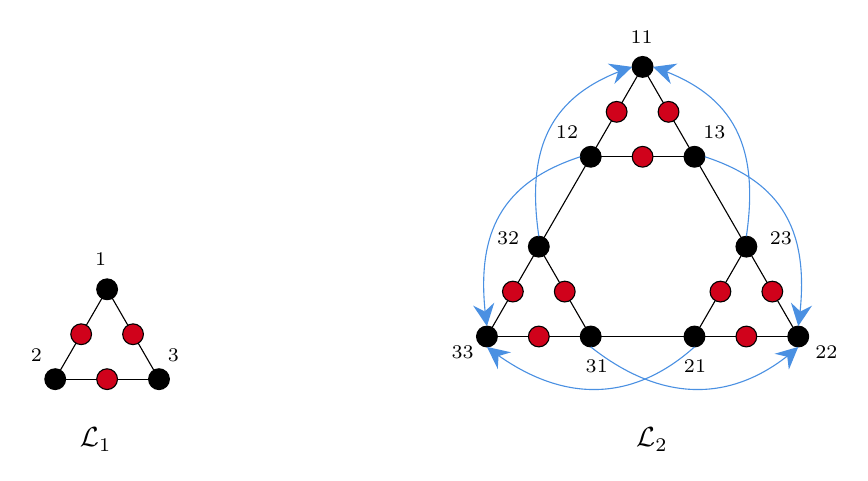
\begin{tikzpicture}[x=0.75pt,y=0.75pt,yscale=-1,xscale=1]
%uncomment if require: \path (0,300); %set diagram left start at 0, and has height of 300

%Straight Lines [id:da582819382900893] 
\draw [fill={rgb, 255:red, 208; green, 2; blue, 27 }  ,fill opacity=1 ]   (455.33,73) -- (505.33,73) ;
%Straight Lines [id:da6363186147188971] 
\draw [fill={rgb, 255:red, 208; green, 2; blue, 27 }  ,fill opacity=1 ]   (480.33,29.7) -- (505.33,73) ;
%Straight Lines [id:da2409715700890418] 
\draw [fill={rgb, 255:red, 208; green, 2; blue, 27 }  ,fill opacity=1 ]   (480.33,29.7) -- (455.33,73) ;
%Shape: Circle [id:dp30893311661910716] 
\draw  [fill={rgb, 255:red, 0; green, 0; blue, 0 }  ,fill opacity=1 ] (475.33,29.7) .. controls (475.33,26.94) and (477.57,24.7) .. (480.33,24.7) .. controls (483.09,24.7) and (485.33,26.94) .. (485.33,29.7) .. controls (485.33,32.46) and (483.09,34.7) .. (480.33,34.7) .. controls (477.57,34.7) and (475.33,32.46) .. (475.33,29.7) -- cycle ;
%Shape: Circle [id:dp9519787435760203] 
\draw  [fill={rgb, 255:red, 0; green, 0; blue, 0 }  ,fill opacity=1 ] (450.33,73) .. controls (450.33,70.24) and (452.57,68) .. (455.33,68) .. controls (458.09,68) and (460.33,70.24) .. (460.33,73) .. controls (460.33,75.76) and (458.09,78) .. (455.33,78) .. controls (452.57,78) and (450.33,75.76) .. (450.33,73) -- cycle ;
%Shape: Circle [id:dp7089231060117445] 
\draw  [fill={rgb, 255:red, 0; green, 0; blue, 0 }  ,fill opacity=1 ] (500.33,73) .. controls (500.33,70.24) and (502.57,68) .. (505.33,68) .. controls (508.09,68) and (510.33,70.24) .. (510.33,73) .. controls (510.33,75.76) and (508.09,78) .. (505.33,78) .. controls (502.57,78) and (500.33,75.76) .. (500.33,73) -- cycle ;
%Straight Lines [id:da33412338200675484] 
\draw    (455.33,73) -- (430.33,116.3) ;
%Straight Lines [id:da48525197654800944] 
\draw [fill={rgb, 255:red, 208; green, 2; blue, 27 }  ,fill opacity=1 ]   (430.33,116.3) -- (405.33,159.6) ;
%Straight Lines [id:da8641302532193023] 
\draw    (505.33,73) -- (530.33,116.3) ;
%Straight Lines [id:da08232291979509676] 
\draw [fill={rgb, 255:red, 208; green, 2; blue, 27 }  ,fill opacity=1 ]   (530.33,116.3) -- (555.33,159.6) ;
%Straight Lines [id:da042199702426409136] 
\draw [fill={rgb, 255:red, 208; green, 2; blue, 27 }  ,fill opacity=1 ]   (530.33,116.3) -- (505.33,159.6) ;
%Straight Lines [id:da03845096660625669] 
\draw [fill={rgb, 255:red, 208; green, 2; blue, 27 }  ,fill opacity=1 ]   (430.33,116.3) -- (455.33,159.6) ;
%Straight Lines [id:da11147524396767561] 
\draw [fill={rgb, 255:red, 208; green, 2; blue, 27 }  ,fill opacity=1 ]   (405.33,159.6) -- (455.33,159.6) ;
%Straight Lines [id:da965556130949931] 
\draw [fill={rgb, 255:red, 208; green, 2; blue, 27 }  ,fill opacity=1 ]   (505.33,159.6) -- (555.33,159.6) ;
%Straight Lines [id:da0950405541587851] 
\draw    (455.33,159.6) -- (505.33,159.6) ;
%Shape: Circle [id:dp36333080496380155] 
\draw  [fill={rgb, 255:red, 0; green, 0; blue, 0 }  ,fill opacity=1 ] (550.33,159.6) .. controls (550.33,156.84) and (552.57,154.6) .. (555.33,154.6) .. controls (558.09,154.6) and (560.33,156.84) .. (560.33,159.6) .. controls (560.33,162.36) and (558.09,164.6) .. (555.33,164.6) .. controls (552.57,164.6) and (550.33,162.36) .. (550.33,159.6) -- cycle ;
%Shape: Circle [id:dp8506659998432795] 
\draw  [fill={rgb, 255:red, 0; green, 0; blue, 0 }  ,fill opacity=1 ] (500.33,159.6) .. controls (500.33,156.84) and (502.57,154.6) .. (505.33,154.6) .. controls (508.09,154.6) and (510.33,156.84) .. (510.33,159.6) .. controls (510.33,162.36) and (508.09,164.6) .. (505.33,164.6) .. controls (502.57,164.6) and (500.33,162.36) .. (500.33,159.6) -- cycle ;
%Shape: Circle [id:dp6204549195542783] 
\draw  [fill={rgb, 255:red, 0; green, 0; blue, 0 }  ,fill opacity=1 ] (525.33,116.3) .. controls (525.33,113.54) and (527.57,111.3) .. (530.33,111.3) .. controls (533.09,111.3) and (535.33,113.54) .. (535.33,116.3) .. controls (535.33,119.06) and (533.09,121.3) .. (530.33,121.3) .. controls (527.57,121.3) and (525.33,119.06) .. (525.33,116.3) -- cycle ;
%Shape: Circle [id:dp2652932116265858] 
\draw  [fill={rgb, 255:red, 0; green, 0; blue, 0 }  ,fill opacity=1 ] (450.33,159.6) .. controls (450.33,156.84) and (452.57,154.6) .. (455.33,154.6) .. controls (458.09,154.6) and (460.33,156.84) .. (460.33,159.6) .. controls (460.33,162.36) and (458.09,164.6) .. (455.33,164.6) .. controls (452.57,164.6) and (450.33,162.36) .. (450.33,159.6) -- cycle ;
%Shape: Circle [id:dp06784631555810572] 
\draw  [fill={rgb, 255:red, 0; green, 0; blue, 0 }  ,fill opacity=1 ] (400.33,159.6) .. controls (400.33,156.84) and (402.57,154.6) .. (405.33,154.6) .. controls (408.09,154.6) and (410.33,156.84) .. (410.33,159.6) .. controls (410.33,162.36) and (408.09,164.6) .. (405.33,164.6) .. controls (402.57,164.6) and (400.33,162.36) .. (400.33,159.6) -- cycle ;
%Shape: Circle [id:dp5652188966162659] 
\draw  [fill={rgb, 255:red, 0; green, 0; blue, 0 }  ,fill opacity=1 ] (425.33,116.3) .. controls (425.33,113.54) and (427.57,111.3) .. (430.33,111.3) .. controls (433.09,111.3) and (435.33,113.54) .. (435.33,116.3) .. controls (435.33,119.06) and (433.09,121.3) .. (430.33,121.3) .. controls (427.57,121.3) and (425.33,119.06) .. (425.33,116.3) -- cycle ;
%Curve Lines [id:da6189894823366382] 
\draw [color={rgb, 255:red, 74; green, 144; blue, 226 }  ,draw opacity=1 ]   (510.33,73) .. controls (547.84,85.26) and (561.29,109.08) .. (555.7,151.95) ;
\draw [shift={(555.33,154.6)}, rotate = 278.3] [fill={rgb, 255:red, 74; green, 144; blue, 226 }  ,fill opacity=1 ][line width=0.08]  [draw opacity=0] (10.72,-5.15) -- (0,0) -- (10.72,5.15) -- (7.12,0) -- cycle    ;
%Curve Lines [id:da24060800083006906] 
\draw [color={rgb, 255:red, 74; green, 144; blue, 226 }  ,draw opacity=1 ]   (488.71,30.86) .. controls (524.38,43.7) and (536.64,68.09) .. (530.33,111.3) ;
\draw [shift={(485.33,29.7)}, rotate = 18.1] [fill={rgb, 255:red, 74; green, 144; blue, 226 }  ,fill opacity=1 ][line width=0.08]  [draw opacity=0] (10.72,-5.15) -- (0,0) -- (10.72,5.15) -- (7.12,0) -- cycle    ;
%Curve Lines [id:da33894788714585133] 
\draw [color={rgb, 255:red, 74; green, 144; blue, 226 }  ,draw opacity=1 ]   (471.96,30.86) .. controls (436.28,43.7) and (424.03,68.09) .. (430.33,111.3) ;
\draw [shift={(475.33,29.7)}, rotate = 161.9] [fill={rgb, 255:red, 74; green, 144; blue, 226 }  ,fill opacity=1 ][line width=0.08]  [draw opacity=0] (10.72,-5.15) -- (0,0) -- (10.72,5.15) -- (7.12,0) -- cycle    ;
%Curve Lines [id:da48491026064962806] 
\draw [color={rgb, 255:red, 74; green, 144; blue, 226 }  ,draw opacity=1 ]   (450.33,73) .. controls (412.83,85.26) and (399.37,109.08) .. (404.97,151.95) ;
\draw [shift={(405.33,154.6)}, rotate = 261.7] [fill={rgb, 255:red, 74; green, 144; blue, 226 }  ,fill opacity=1 ][line width=0.08]  [draw opacity=0] (10.72,-5.15) -- (0,0) -- (10.72,5.15) -- (7.12,0) -- cycle    ;
%Curve Lines [id:da022467158338492776] 
\draw [color={rgb, 255:red, 74; green, 144; blue, 226 }  ,draw opacity=1 ]   (505.33,164.6) .. controls (475.96,190.96) and (442.05,192.45) .. (407.45,166.24) ;
\draw [shift={(405.33,164.6)}, rotate = 38.3] [fill={rgb, 255:red, 74; green, 144; blue, 226 }  ,fill opacity=1 ][line width=0.08]  [draw opacity=0] (10.72,-5.15) -- (0,0) -- (10.72,5.15) -- (7.12,0) -- cycle    ;
%Curve Lines [id:da7803550651990034] 
\draw [color={rgb, 255:red, 74; green, 144; blue, 226 }  ,draw opacity=1 ]   (552.62,166.95) .. controls (523.28,191.53) and (489.6,191.67) .. (455.33,164.6) ;
\draw [shift={(555.33,164.6)}, rotate = 138.1] [fill={rgb, 255:red, 74; green, 144; blue, 226 }  ,fill opacity=1 ][line width=0.08]  [draw opacity=0] (10.72,-5.15) -- (0,0) -- (10.72,5.15) -- (7.12,0) -- cycle    ;
%Shape: Circle [id:dp9501270285087915] 
\draw  [fill={rgb, 255:red, 208; green, 2; blue, 27 }  ,fill opacity=1 ] (487.83,51.35) .. controls (487.83,48.59) and (490.07,46.35) .. (492.83,46.35) .. controls (495.59,46.35) and (497.83,48.59) .. (497.83,51.35) .. controls (497.83,54.11) and (495.59,56.35) .. (492.83,56.35) .. controls (490.07,56.35) and (487.83,54.11) .. (487.83,51.35) -- cycle ;
%Shape: Circle [id:dp5318859502866085] 
\draw  [fill={rgb, 255:red, 208; green, 2; blue, 27 }  ,fill opacity=1 ] (475.33,73) .. controls (475.33,70.24) and (477.57,68) .. (480.33,68) .. controls (483.09,68) and (485.33,70.24) .. (485.33,73) .. controls (485.33,75.76) and (483.09,78) .. (480.33,78) .. controls (477.57,78) and (475.33,75.76) .. (475.33,73) -- cycle ;
%Shape: Circle [id:dp7700797012983556] 
\draw  [fill={rgb, 255:red, 208; green, 2; blue, 27 }  ,fill opacity=1 ] (537.83,137.95) .. controls (537.83,135.19) and (540.07,132.95) .. (542.83,132.95) .. controls (545.59,132.95) and (547.83,135.19) .. (547.83,137.95) .. controls (547.83,140.71) and (545.59,142.95) .. (542.83,142.95) .. controls (540.07,142.95) and (537.83,140.71) .. (537.83,137.95) -- cycle ;
%Shape: Circle [id:dp7549766955423654] 
\draw  [fill={rgb, 255:red, 208; green, 2; blue, 27 }  ,fill opacity=1 ] (462.83,51.35) .. controls (462.83,48.59) and (465.07,46.35) .. (467.83,46.35) .. controls (470.59,46.35) and (472.83,48.59) .. (472.83,51.35) .. controls (472.83,54.11) and (470.59,56.35) .. (467.83,56.35) .. controls (465.07,56.35) and (462.83,54.11) .. (462.83,51.35) -- cycle ;
%Shape: Circle [id:dp7348205710166487] 
\draw  [fill={rgb, 255:red, 208; green, 2; blue, 27 }  ,fill opacity=1 ] (512.83,137.95) .. controls (512.83,135.19) and (515.07,132.95) .. (517.83,132.95) .. controls (520.59,132.95) and (522.83,135.19) .. (522.83,137.95) .. controls (522.83,140.71) and (520.59,142.95) .. (517.83,142.95) .. controls (515.07,142.95) and (512.83,140.71) .. (512.83,137.95) -- cycle ;
%Shape: Circle [id:dp24817732108140267] 
\draw  [fill={rgb, 255:red, 208; green, 2; blue, 27 }  ,fill opacity=1 ] (525.33,159.6) .. controls (525.33,156.84) and (527.57,154.6) .. (530.33,154.6) .. controls (533.09,154.6) and (535.33,156.84) .. (535.33,159.6) .. controls (535.33,162.36) and (533.09,164.6) .. (530.33,164.6) .. controls (527.57,164.6) and (525.33,162.36) .. (525.33,159.6) -- cycle ;
%Shape: Circle [id:dp9000837085734259] 
\draw  [fill={rgb, 255:red, 208; green, 2; blue, 27 }  ,fill opacity=1 ] (425.33,159.6) .. controls (425.33,156.84) and (427.57,154.6) .. (430.33,154.6) .. controls (433.09,154.6) and (435.33,156.84) .. (435.33,159.6) .. controls (435.33,162.36) and (433.09,164.6) .. (430.33,164.6) .. controls (427.57,164.6) and (425.33,162.36) .. (425.33,159.6) -- cycle ;
%Shape: Circle [id:dp20337902659167173] 
\draw  [fill={rgb, 255:red, 208; green, 2; blue, 27 }  ,fill opacity=1 ] (412.83,137.95) .. controls (412.83,135.19) and (415.07,132.95) .. (417.83,132.95) .. controls (420.59,132.95) and (422.83,135.19) .. (422.83,137.95) .. controls (422.83,140.71) and (420.59,142.95) .. (417.83,142.95) .. controls (415.07,142.95) and (412.83,140.71) .. (412.83,137.95) -- cycle ;
%Shape: Circle [id:dp36524254827900804] 
\draw  [fill={rgb, 255:red, 208; green, 2; blue, 27 }  ,fill opacity=1 ] (437.83,137.95) .. controls (437.83,135.19) and (440.07,132.95) .. (442.83,132.95) .. controls (445.59,132.95) and (447.83,135.19) .. (447.83,137.95) .. controls (447.83,140.71) and (445.59,142.95) .. (442.83,142.95) .. controls (440.07,142.95) and (437.83,140.71) .. (437.83,137.95) -- cycle ;

%Straight Lines [id:da2789728878883566] 
\draw [fill={rgb, 255:red, 208; green, 2; blue, 27 }  ,fill opacity=1 ]   (197.33,180.15) -- (247.33,180.15) ;
%Straight Lines [id:da5802994965633916] 
\draw [fill={rgb, 255:red, 208; green, 2; blue, 27 }  ,fill opacity=1 ]   (222.33,136.85) -- (247.33,180.15) ;
%Straight Lines [id:da16690551925874586] 
\draw [fill={rgb, 255:red, 208; green, 2; blue, 27 }  ,fill opacity=1 ]   (222.33,136.85) -- (197.33,180.15) ;
%Shape: Circle [id:dp7927550621196953] 
\draw  [fill={rgb, 255:red, 0; green, 0; blue, 0 }  ,fill opacity=1 ] (217.33,136.85) .. controls (217.33,134.09) and (219.57,131.85) .. (222.33,131.85) .. controls (225.09,131.85) and (227.33,134.09) .. (227.33,136.85) .. controls (227.33,139.61) and (225.09,141.85) .. (222.33,141.85) .. controls (219.57,141.85) and (217.33,139.61) .. (217.33,136.85) -- cycle ;
%Shape: Circle [id:dp13109108888045662] 
\draw  [fill={rgb, 255:red, 0; green, 0; blue, 0 }  ,fill opacity=1 ] (192.33,180.15) .. controls (192.33,177.39) and (194.57,175.15) .. (197.33,175.15) .. controls (200.09,175.15) and (202.33,177.39) .. (202.33,180.15) .. controls (202.33,182.91) and (200.09,185.15) .. (197.33,185.15) .. controls (194.57,185.15) and (192.33,182.91) .. (192.33,180.15) -- cycle ;
%Shape: Circle [id:dp3994478644973736] 
\draw  [fill={rgb, 255:red, 0; green, 0; blue, 0 }  ,fill opacity=1 ] (242.33,180.15) .. controls (242.33,177.39) and (244.57,175.15) .. (247.33,175.15) .. controls (250.09,175.15) and (252.33,177.39) .. (252.33,180.15) .. controls (252.33,182.91) and (250.09,185.15) .. (247.33,185.15) .. controls (244.57,185.15) and (242.33,182.91) .. (242.33,180.15) -- cycle ;
%Shape: Circle [id:dp9959797529549808] 
\draw  [fill={rgb, 255:red, 208; green, 2; blue, 27 }  ,fill opacity=1 ] (229.83,158.5) .. controls (229.83,155.74) and (232.07,153.5) .. (234.83,153.5) .. controls (237.59,153.5) and (239.83,155.74) .. (239.83,158.5) .. controls (239.83,161.26) and (237.59,163.5) .. (234.83,163.5) .. controls (232.07,163.5) and (229.83,161.26) .. (229.83,158.5) -- cycle ;
%Shape: Circle [id:dp34894570798222113] 
\draw  [fill={rgb, 255:red, 208; green, 2; blue, 27 }  ,fill opacity=1 ] (217.33,180.15) .. controls (217.33,177.39) and (219.57,175.15) .. (222.33,175.15) .. controls (225.09,175.15) and (227.33,177.39) .. (227.33,180.15) .. controls (227.33,182.91) and (225.09,185.15) .. (222.33,185.15) .. controls (219.57,185.15) and (217.33,182.91) .. (217.33,180.15) -- cycle ;
%Shape: Circle [id:dp8154111462983866] 
\draw  [fill={rgb, 255:red, 208; green, 2; blue, 27 }  ,fill opacity=1 ] (204.83,158.5) .. controls (204.83,155.74) and (207.07,153.5) .. (209.83,153.5) .. controls (212.59,153.5) and (214.83,155.74) .. (214.83,158.5) .. controls (214.83,161.26) and (212.59,163.5) .. (209.83,163.5) .. controls (207.07,163.5) and (204.83,161.26) .. (204.83,158.5) -- cycle ;


% Text Node
\draw (208,202.4) node [anchor=north west][inner sep=0.75pt]    {$\mathcal{L}_{1}$};
% Text Node
\draw (476,202.4) node [anchor=north west][inner sep=0.75pt]    {$\mathcal{L}_{2}$};
% Text Node
\draw (215.33,118.22) node [anchor=north west][inner sep=0.75pt]  [font=\scriptsize]  {$1$};
% Text Node
\draw (250.33,164.22) node [anchor=north west][inner sep=0.75pt]  [font=\scriptsize]  {$3$};
% Text Node
\draw (184.33,164.22) node [anchor=north west][inner sep=0.75pt]  [font=\scriptsize]  {$2$};
% Text Node
\draw (473.33,11.07) node [anchor=north west][inner sep=0.75pt]  [font=\scriptsize]  {$11$};
% Text Node
\draw (562.33,163.07) node [anchor=north west][inner sep=0.75pt]  [font=\scriptsize]  {$22$};
% Text Node
\draw (387,163.07) node [anchor=north west][inner sep=0.75pt]  [font=\scriptsize]  {$33$};
% Text Node
\draw (508.33,57.07) node [anchor=north west][inner sep=0.75pt]  [font=\scriptsize]  {$13$};
% Text Node
\draw (437.33,57.07) node [anchor=north west][inner sep=0.75pt]  [font=\scriptsize]  {$12$};
% Text Node
\draw (499,169.67) node [anchor=north west][inner sep=0.75pt]  [font=\scriptsize]  {$21$};
% Text Node
\draw (540.33,108.07) node [anchor=north west][inner sep=0.75pt]  [font=\scriptsize]  {$23$};
% Text Node
\draw (451.67,169.67) node [anchor=north west][inner sep=0.75pt]  [font=\scriptsize]  {$31$};
% Text Node
\draw (409,108.07) node [anchor=north west][inner sep=0.75pt]  [font=\scriptsize]  {$32$};


\end{tikzpicture}
    \caption{ the Lucas-Tower graphs $\mathcal{L}_{1}$ and $\mathcal{L}_{2}$}
    \label{fig:graph_lucas}
\end{figure}

The same for Jacobsthal-Tower graphs and Pell-Tower graphs, associated respectively to the Towers of Jacobsthal and Pell, they can be generated from $\mathcal{F}_{n}$ by deleting the forbidding arcs that violate the corresponding rules. Figure \ref{fig:graph_jaco-pell} illustrates the Jacobsthal-Tower graph $\mathcal{J}_{2}$  and Pell-Tower graph  $\mathcal{P}_{2}$. 




\begin{figure}[H]
    \centering
    

\tikzset{every picture/.style={line width=0.75pt}} %set default line width to 0.75pt        

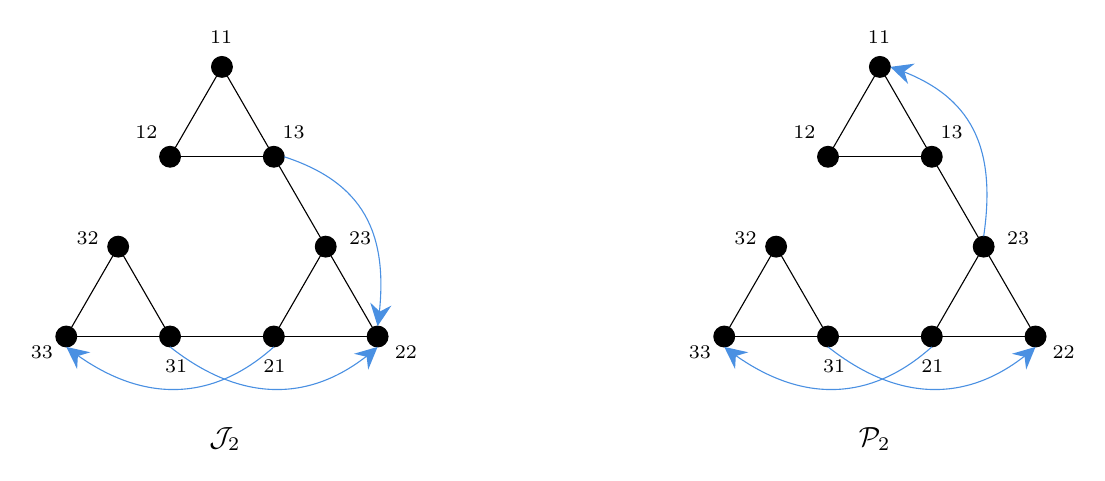
\begin{tikzpicture}[x=0.75pt,y=0.75pt,yscale=-1,xscale=1]
%uncomment if require: \path (0,548); %set diagram left start at 0, and has height of 548

%Straight Lines [id:da975491716684024] 
\draw [fill={rgb, 255:red, 208; green, 2; blue, 27 }  ,fill opacity=1 ]   (140.33,98.24) -- (190.33,98.24) ;
%Straight Lines [id:da24333401847433977] 
\draw [fill={rgb, 255:red, 208; green, 2; blue, 27 }  ,fill opacity=1 ]   (165.33,54.94) -- (190.33,98.24) ;
%Straight Lines [id:da6709939745284248] 
\draw [fill={rgb, 255:red, 208; green, 2; blue, 27 }  ,fill opacity=1 ]   (165.33,54.94) -- (140.33,98.24) ;
%Shape: Circle [id:dp533570779991716] 
\draw  [fill={rgb, 255:red, 0; green, 0; blue, 0 }  ,fill opacity=1 ] (160.33,54.94) .. controls (160.33,52.18) and (162.57,49.94) .. (165.33,49.94) .. controls (168.09,49.94) and (170.33,52.18) .. (170.33,54.94) .. controls (170.33,57.7) and (168.09,59.94) .. (165.33,59.94) .. controls (162.57,59.94) and (160.33,57.7) .. (160.33,54.94) -- cycle ;
%Shape: Circle [id:dp9426032090854817] 
\draw  [fill={rgb, 255:red, 0; green, 0; blue, 0 }  ,fill opacity=1 ] (135.33,98.24) .. controls (135.33,95.48) and (137.57,93.24) .. (140.33,93.24) .. controls (143.09,93.24) and (145.33,95.48) .. (145.33,98.24) .. controls (145.33,101) and (143.09,103.24) .. (140.33,103.24) .. controls (137.57,103.24) and (135.33,101) .. (135.33,98.24) -- cycle ;
%Shape: Circle [id:dp22765353488254747] 
\draw  [fill={rgb, 255:red, 0; green, 0; blue, 0 }  ,fill opacity=1 ] (185.33,98.24) .. controls (185.33,95.48) and (187.57,93.24) .. (190.33,93.24) .. controls (193.09,93.24) and (195.33,95.48) .. (195.33,98.24) .. controls (195.33,101) and (193.09,103.24) .. (190.33,103.24) .. controls (187.57,103.24) and (185.33,101) .. (185.33,98.24) -- cycle ;
%Straight Lines [id:da24320423104510702] 
\draw [fill={rgb, 255:red, 208; green, 2; blue, 27 }  ,fill opacity=1 ]   (115.33,141.54) -- (90.33,184.84) ;
%Straight Lines [id:da9790391915729273] 
\draw    (190.33,98.24) -- (215.33,141.54) ;
%Straight Lines [id:da8689695720463988] 
\draw [fill={rgb, 255:red, 208; green, 2; blue, 27 }  ,fill opacity=1 ]   (215.33,141.54) -- (240.33,184.84) ;
%Straight Lines [id:da6376267112447536] 
\draw [fill={rgb, 255:red, 208; green, 2; blue, 27 }  ,fill opacity=1 ]   (215.33,141.54) -- (190.33,184.84) ;
%Straight Lines [id:da4847559935143244] 
\draw [fill={rgb, 255:red, 208; green, 2; blue, 27 }  ,fill opacity=1 ]   (115.33,141.54) -- (140.33,184.84) ;
%Straight Lines [id:da968222756401508] 
\draw [fill={rgb, 255:red, 208; green, 2; blue, 27 }  ,fill opacity=1 ]   (90.33,184.84) -- (140.33,184.84) ;
%Straight Lines [id:da32037613995251646] 
\draw [fill={rgb, 255:red, 208; green, 2; blue, 27 }  ,fill opacity=1 ]   (190.33,184.84) -- (240.33,184.84) ;
%Straight Lines [id:da6652531696436412] 
\draw    (140.33,184.84) -- (190.33,184.84) ;
%Shape: Circle [id:dp34096249146943314] 
\draw  [fill={rgb, 255:red, 0; green, 0; blue, 0 }  ,fill opacity=1 ] (235.33,184.84) .. controls (235.33,182.08) and (237.57,179.84) .. (240.33,179.84) .. controls (243.09,179.84) and (245.33,182.08) .. (245.33,184.84) .. controls (245.33,187.61) and (243.09,189.84) .. (240.33,189.84) .. controls (237.57,189.84) and (235.33,187.61) .. (235.33,184.84) -- cycle ;
%Shape: Circle [id:dp07138382608731342] 
\draw  [fill={rgb, 255:red, 0; green, 0; blue, 0 }  ,fill opacity=1 ] (185.33,184.84) .. controls (185.33,182.08) and (187.57,179.84) .. (190.33,179.84) .. controls (193.09,179.84) and (195.33,182.08) .. (195.33,184.84) .. controls (195.33,187.61) and (193.09,189.84) .. (190.33,189.84) .. controls (187.57,189.84) and (185.33,187.61) .. (185.33,184.84) -- cycle ;
%Shape: Circle [id:dp08429888664223473] 
\draw  [fill={rgb, 255:red, 0; green, 0; blue, 0 }  ,fill opacity=1 ] (210.33,141.54) .. controls (210.33,138.78) and (212.57,136.54) .. (215.33,136.54) .. controls (218.09,136.54) and (220.33,138.78) .. (220.33,141.54) .. controls (220.33,144.31) and (218.09,146.54) .. (215.33,146.54) .. controls (212.57,146.54) and (210.33,144.31) .. (210.33,141.54) -- cycle ;
%Shape: Circle [id:dp8726438346773229] 
\draw  [fill={rgb, 255:red, 0; green, 0; blue, 0 }  ,fill opacity=1 ] (135.33,184.84) .. controls (135.33,182.08) and (137.57,179.84) .. (140.33,179.84) .. controls (143.09,179.84) and (145.33,182.08) .. (145.33,184.84) .. controls (145.33,187.61) and (143.09,189.84) .. (140.33,189.84) .. controls (137.57,189.84) and (135.33,187.61) .. (135.33,184.84) -- cycle ;
%Shape: Circle [id:dp11453731238812614] 
\draw  [fill={rgb, 255:red, 0; green, 0; blue, 0 }  ,fill opacity=1 ] (85.33,184.84) .. controls (85.33,182.08) and (87.57,179.84) .. (90.33,179.84) .. controls (93.09,179.84) and (95.33,182.08) .. (95.33,184.84) .. controls (95.33,187.61) and (93.09,189.84) .. (90.33,189.84) .. controls (87.57,189.84) and (85.33,187.61) .. (85.33,184.84) -- cycle ;
%Shape: Circle [id:dp13815270430200122] 
\draw  [fill={rgb, 255:red, 0; green, 0; blue, 0 }  ,fill opacity=1 ] (110.33,141.54) .. controls (110.33,138.78) and (112.57,136.54) .. (115.33,136.54) .. controls (118.09,136.54) and (120.33,138.78) .. (120.33,141.54) .. controls (120.33,144.31) and (118.09,146.54) .. (115.33,146.54) .. controls (112.57,146.54) and (110.33,144.31) .. (110.33,141.54) -- cycle ;
%Curve Lines [id:da4868898702177904] 
\draw [color={rgb, 255:red, 74; green, 144; blue, 226 }  ,draw opacity=1 ]   (195.33,98.24) .. controls (232.84,110.5) and (246.29,134.32) .. (240.7,177.2) ;
\draw [shift={(240.33,179.84)}, rotate = 278.3] [fill={rgb, 255:red, 74; green, 144; blue, 226 }  ,fill opacity=1 ][line width=0.08]  [draw opacity=0] (10.72,-5.15) -- (0,0) -- (10.72,5.15) -- (7.12,0) -- cycle    ;
%Curve Lines [id:da776047539580841] 
\draw [color={rgb, 255:red, 74; green, 144; blue, 226 }  ,draw opacity=1 ]   (190.33,189.84) .. controls (160.96,216.2) and (127.05,217.7) .. (92.45,191.48) ;
\draw [shift={(90.33,189.84)}, rotate = 38.3] [fill={rgb, 255:red, 74; green, 144; blue, 226 }  ,fill opacity=1 ][line width=0.08]  [draw opacity=0] (10.72,-5.15) -- (0,0) -- (10.72,5.15) -- (7.12,0) -- cycle    ;
%Curve Lines [id:da4085033920640422] 
\draw [color={rgb, 255:red, 74; green, 144; blue, 226 }  ,draw opacity=1 ]   (237.62,192.2) .. controls (208.28,216.77) and (174.6,216.91) .. (140.33,189.84) ;
\draw [shift={(240.33,189.84)}, rotate = 138.1] [fill={rgb, 255:red, 74; green, 144; blue, 226 }  ,fill opacity=1 ][line width=0.08]  [draw opacity=0] (10.72,-5.15) -- (0,0) -- (10.72,5.15) -- (7.12,0) -- cycle    ;

%Straight Lines [id:da43659107115763973] 
\draw    (457.33,98.24) -- (507.33,98.24) ;
%Straight Lines [id:da8705509571333112] 
\draw    (482.33,54.94) -- (507.33,98.24) ;
%Straight Lines [id:da670040381431358] 
\draw    (482.33,54.94) -- (457.33,98.24) ;
%Shape: Circle [id:dp9814000792805107] 
\draw  [fill={rgb, 255:red, 0; green, 0; blue, 0 }  ,fill opacity=1 ] (477.33,54.94) .. controls (477.33,52.18) and (479.57,49.94) .. (482.33,49.94) .. controls (485.09,49.94) and (487.33,52.18) .. (487.33,54.94) .. controls (487.33,57.7) and (485.09,59.94) .. (482.33,59.94) .. controls (479.57,59.94) and (477.33,57.7) .. (477.33,54.94) -- cycle ;
%Shape: Circle [id:dp9052593368214028] 
\draw  [fill={rgb, 255:red, 0; green, 0; blue, 0 }  ,fill opacity=1 ] (452.33,98.24) .. controls (452.33,95.48) and (454.57,93.24) .. (457.33,93.24) .. controls (460.09,93.24) and (462.33,95.48) .. (462.33,98.24) .. controls (462.33,101) and (460.09,103.24) .. (457.33,103.24) .. controls (454.57,103.24) and (452.33,101) .. (452.33,98.24) -- cycle ;
%Shape: Circle [id:dp09153509695315232] 
\draw  [fill={rgb, 255:red, 0; green, 0; blue, 0 }  ,fill opacity=1 ] (502.33,98.24) .. controls (502.33,95.48) and (504.57,93.24) .. (507.33,93.24) .. controls (510.09,93.24) and (512.33,95.48) .. (512.33,98.24) .. controls (512.33,101) and (510.09,103.24) .. (507.33,103.24) .. controls (504.57,103.24) and (502.33,101) .. (502.33,98.24) -- cycle ;
%Straight Lines [id:da4885611002171404] 
\draw    (432.33,141.54) -- (407.33,184.84) ;
%Straight Lines [id:da6749851436896508] 
\draw    (507.33,98.24) -- (532.33,141.54) ;
%Straight Lines [id:da20163439320392884] 
\draw    (532.33,141.54) -- (557.33,184.84) ;
%Straight Lines [id:da45241045044707695] 
\draw    (532.33,141.54) -- (507.33,184.84) ;
%Straight Lines [id:da8946563775088479] 
\draw    (432.33,141.54) -- (457.33,184.84) ;
%Straight Lines [id:da1309497018168646] 
\draw    (407.33,184.84) -- (457.33,184.84) ;
%Straight Lines [id:da9535533415940451] 
\draw    (507.33,184.84) -- (557.33,184.84) ;
%Straight Lines [id:da5918616364318543] 
\draw    (457.33,184.84) -- (507.33,184.84) ;
%Shape: Circle [id:dp1707094051735225] 
\draw  [fill={rgb, 255:red, 0; green, 0; blue, 0 }  ,fill opacity=1 ] (552.33,184.84) .. controls (552.33,182.08) and (554.57,179.84) .. (557.33,179.84) .. controls (560.09,179.84) and (562.33,182.08) .. (562.33,184.84) .. controls (562.33,187.61) and (560.09,189.84) .. (557.33,189.84) .. controls (554.57,189.84) and (552.33,187.61) .. (552.33,184.84) -- cycle ;
%Shape: Circle [id:dp6689130175111455] 
\draw  [fill={rgb, 255:red, 0; green, 0; blue, 0 }  ,fill opacity=1 ] (502.33,184.84) .. controls (502.33,182.08) and (504.57,179.84) .. (507.33,179.84) .. controls (510.09,179.84) and (512.33,182.08) .. (512.33,184.84) .. controls (512.33,187.61) and (510.09,189.84) .. (507.33,189.84) .. controls (504.57,189.84) and (502.33,187.61) .. (502.33,184.84) -- cycle ;
%Shape: Circle [id:dp38339482371537104] 
\draw  [fill={rgb, 255:red, 0; green, 0; blue, 0 }  ,fill opacity=1 ] (527.33,141.54) .. controls (527.33,138.78) and (529.57,136.54) .. (532.33,136.54) .. controls (535.09,136.54) and (537.33,138.78) .. (537.33,141.54) .. controls (537.33,144.31) and (535.09,146.54) .. (532.33,146.54) .. controls (529.57,146.54) and (527.33,144.31) .. (527.33,141.54) -- cycle ;
%Shape: Circle [id:dp7180746192026639] 
\draw  [fill={rgb, 255:red, 0; green, 0; blue, 0 }  ,fill opacity=1 ] (452.33,184.84) .. controls (452.33,182.08) and (454.57,179.84) .. (457.33,179.84) .. controls (460.09,179.84) and (462.33,182.08) .. (462.33,184.84) .. controls (462.33,187.61) and (460.09,189.84) .. (457.33,189.84) .. controls (454.57,189.84) and (452.33,187.61) .. (452.33,184.84) -- cycle ;
%Shape: Circle [id:dp36743110976028226] 
\draw  [fill={rgb, 255:red, 0; green, 0; blue, 0 }  ,fill opacity=1 ] (402.33,184.84) .. controls (402.33,182.08) and (404.57,179.84) .. (407.33,179.84) .. controls (410.09,179.84) and (412.33,182.08) .. (412.33,184.84) .. controls (412.33,187.61) and (410.09,189.84) .. (407.33,189.84) .. controls (404.57,189.84) and (402.33,187.61) .. (402.33,184.84) -- cycle ;
%Shape: Circle [id:dp8263796839485265] 
\draw  [fill={rgb, 255:red, 0; green, 0; blue, 0 }  ,fill opacity=1 ] (427.33,141.54) .. controls (427.33,138.78) and (429.57,136.54) .. (432.33,136.54) .. controls (435.09,136.54) and (437.33,138.78) .. (437.33,141.54) .. controls (437.33,144.31) and (435.09,146.54) .. (432.33,146.54) .. controls (429.57,146.54) and (427.33,144.31) .. (427.33,141.54) -- cycle ;
%Curve Lines [id:da7278452179566555] 
\draw [color={rgb, 255:red, 74; green, 144; blue, 226 }  ,draw opacity=1 ]   (490.71,56.1) .. controls (526.38,68.94) and (538.64,93.33) .. (532.33,136.54) ;
\draw [shift={(487.33,54.94)}, rotate = 18.1] [fill={rgb, 255:red, 74; green, 144; blue, 226 }  ,fill opacity=1 ][line width=0.08]  [draw opacity=0] (10.72,-5.15) -- (0,0) -- (10.72,5.15) -- (7.12,0) -- cycle    ;
%Curve Lines [id:da39160252250743177] 
\draw [color={rgb, 255:red, 74; green, 144; blue, 226 }  ,draw opacity=1 ]   (507.33,189.84) .. controls (477.96,216.2) and (444.05,217.7) .. (409.45,191.48) ;
\draw [shift={(407.33,189.84)}, rotate = 38.3] [fill={rgb, 255:red, 74; green, 144; blue, 226 }  ,fill opacity=1 ][line width=0.08]  [draw opacity=0] (10.72,-5.15) -- (0,0) -- (10.72,5.15) -- (7.12,0) -- cycle    ;
%Curve Lines [id:da0266934450502192] 
\draw [color={rgb, 255:red, 74; green, 144; blue, 226 }  ,draw opacity=1 ]   (554.62,192.2) .. controls (525.28,216.77) and (491.6,216.91) .. (457.33,189.84) ;
\draw [shift={(557.33,189.84)}, rotate = 138.1] [fill={rgb, 255:red, 74; green, 144; blue, 226 }  ,fill opacity=1 ][line width=0.08]  [draw opacity=0] (10.72,-5.15) -- (0,0) -- (10.72,5.15) -- (7.12,0) -- cycle    ;


% Text Node
\draw (158,227.4) node [anchor=north west][inner sep=0.75pt]    {$\mathcal{J}_{2}$};
% Text Node
\draw (94,133.31) node [anchor=north west][inner sep=0.75pt]  [font=\scriptsize]  {$32$};
% Text Node
\draw (136.67,194.91) node [anchor=north west][inner sep=0.75pt]  [font=\scriptsize]  {$31$};
% Text Node
\draw (225.33,133.31) node [anchor=north west][inner sep=0.75pt]  [font=\scriptsize]  {$23$};
% Text Node
\draw (184,194.91) node [anchor=north west][inner sep=0.75pt]  [font=\scriptsize]  {$21$};
% Text Node
\draw (122.33,82.31) node [anchor=north west][inner sep=0.75pt]  [font=\scriptsize]  {$12$};
% Text Node
\draw (193.33,82.31) node [anchor=north west][inner sep=0.75pt]  [font=\scriptsize]  {$13$};
% Text Node
\draw (72,188.31) node [anchor=north west][inner sep=0.75pt]  [font=\scriptsize]  {$33$};
% Text Node
\draw (247.33,188.31) node [anchor=north west][inner sep=0.75pt]  [font=\scriptsize]  {$22$};
% Text Node
\draw (158.33,36.31) node [anchor=north west][inner sep=0.75pt]  [font=\scriptsize]  {$11$};
% Text Node
\draw (471,227.4) node [anchor=north west][inner sep=0.75pt]    {$\mathcal{P}_{2}$};
% Text Node
\draw (411,133.31) node [anchor=north west][inner sep=0.75pt]  [font=\scriptsize]  {$32$};
% Text Node
\draw (453.67,194.91) node [anchor=north west][inner sep=0.75pt]  [font=\scriptsize]  {$31$};
% Text Node
\draw (542.33,133.31) node [anchor=north west][inner sep=0.75pt]  [font=\scriptsize]  {$23$};
% Text Node
\draw (501,194.91) node [anchor=north west][inner sep=0.75pt]  [font=\scriptsize]  {$21$};
% Text Node
\draw (439.33,82.31) node [anchor=north west][inner sep=0.75pt]  [font=\scriptsize]  {$12$};
% Text Node
\draw (510.33,82.31) node [anchor=north west][inner sep=0.75pt]  [font=\scriptsize]  {$13$};
% Text Node
\draw (389,188.31) node [anchor=north west][inner sep=0.75pt]  [font=\scriptsize]  {$33$};
% Text Node
\draw (564.33,188.31) node [anchor=north west][inner sep=0.75pt]  [font=\scriptsize]  {$22$};
% Text Node
\draw (475.33,36.31) node [anchor=north west][inner sep=0.75pt]  [font=\scriptsize]  {$11$};


\end{tikzpicture}
    \caption{Jacobsthal-Tower graph $\mathcal{J}_{2}$ and Pell-Tower graph  $\mathcal{P}_{2}$}
    \label{fig:graph_jaco-pell}
\end{figure}



\section{Conclusion, and  a possible  generalization for further works}
A new combinatorial interpretation of the four famous numbers, Fibonacci, Lucas, Jacobsthal, and Pell numbers,  was presented in this work, through the discs and pegs of the framework of the Tower of Hanoi puzzle. The variants presented in this work produce new graph classes, that seem to have very interesting recursive aspects. Studying these new variants involved multiple fields of mathematics, such as algorithms, combinatorics, and graph theory, which proved the interest of these variants.  

The sequences of Fibonacci, Lucas, Jacobsthal, and Pell are particular cases of the Lucas sequences $U_{n}(P,Q)$ (first kind) and $ V_{n}(P,Q)$ (second kind) defined by the following recurrences,  

\begin{equation}U_{n}(P,Q)=
    \begin{cases}
    0&if\;n=0,\\
    1&if\;n=1,\\
    P U_{n-1}(P,Q)-Q U_{n-2}(P,Q)&if\;n\geq 2,\\
    \end{cases}
\end{equation}
 \begin{equation}V_{n}(P,Q)=
    \begin{cases}
    2&if\;n=0,\\
    P&if\;n=1,\\
    P V_{n-1}(P,Q)-Q V_{n-2}(P,Q)&if\;n\geq 2,\\
    \end{cases}
\end{equation}

where $P$ and $Q$ are fixed integers. We can see that $F_{n}=U_{n}(1,-1)$, $L_{n}=V_{n}(1,-1)$,  $J_{n}=U_{n}(1,-2)$, and $J_{n}=U_{n}(2,-1)$. Even the sequence of Merssene numbers related to the length of the optimal solution of the classical Tower of Hanoi is a particular case of Lucas sequences, where $M_{n}=U_{n}(3, 2)$.

Thus, a natural question arises for  further generalization: Find a way to define alternative natural rules for the classical Tower of Hanoi problem such that the length of the optimal solution corresponds to some Lucas sequence $U_{n}(P,Q)$ and $ V_{n}(P,Q)$ fixed a priori. The rules to be fixed should take into consideration the values of $P$ and $Q$, as well as the and whether the kind (first or second) of the priori fixed sequence.









 




\printbibliography[
heading=bibintoc
]



\appendix
\section{Appendix: Illustrations of the optimal solutions using discs and pegs}


\subsection{Tower of Fibonacci}
\begin{figure}[H]
    \centering
    

\tikzset{every picture/.style={line width=0.75pt}} %set default line width to 0.75pt        

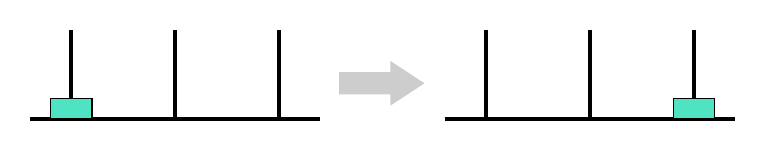
\begin{tikzpicture}[x=0.75pt,y=0.75pt,yscale=-1,xscale=1]
%uncomment if require: \path (0,232); %set diagram left start at 0, and has height of 232

%Straight Lines [id:da5061956555306579] 
\draw [line width=1.5]    (0,43) -- (140,43) ;
%Straight Lines [id:da14873551291186748] 
\draw [line width=1.5]    (20,43) -- (20,0) ;
%Straight Lines [id:da04349752359754144] 
\draw [line width=1.5]    (70,43) -- (70,0) ;
%Straight Lines [id:da8186372502878208] 
\draw [line width=1.5]    (120,43) -- (120,0) ;
%Shape: Rectangle [id:dp3498756304062225] 
\draw  [fill={rgb, 255:red, 80; green, 227; blue, 194 }  ,fill opacity=1 ] (10,33) -- (30,33) -- (30,43) -- (10,43) -- cycle ;
%Straight Lines [id:da2647400328890377] 
\draw [line width=1.5]    (200,43) -- (340,43) ;
%Straight Lines [id:da6438813986564005] 
\draw [line width=1.5]    (220,43) -- (220,0) ;
%Straight Lines [id:da6590761317241682] 
\draw [line width=1.5]    (270,43) -- (270,0) ;
%Straight Lines [id:da8132147600253368] 
\draw [line width=1.5]    (320,43) -- (320,0) ;
%Shape: Rectangle [id:dp6568998296061901] 
\draw  [fill={rgb, 255:red, 80; green, 227; blue, 194 }  ,fill opacity=1 ] (310,33) -- (330,33) -- (330,43) -- (310,43) -- cycle ;
%Right Arrow [id:dp01322583224439633] 
\draw  [draw opacity=0][fill={rgb, 255:red, 155; green, 155; blue, 155 }  ,fill opacity=0.5 ] (149,20.4) -- (173.71,20.4) -- (173.71,15) -- (190.18,25.8) -- (173.71,36.59) -- (173.71,31.19) -- (149,31.19) -- cycle ;




\end{tikzpicture}
    \caption{The solution of the Tower of Fibonacci with $n=1$ discs.}
\end{figure}

\begin{figure}[H]
    \centering
    

\tikzset{every picture/.style={line width=0.75pt}} %set default line width to 0.75pt        

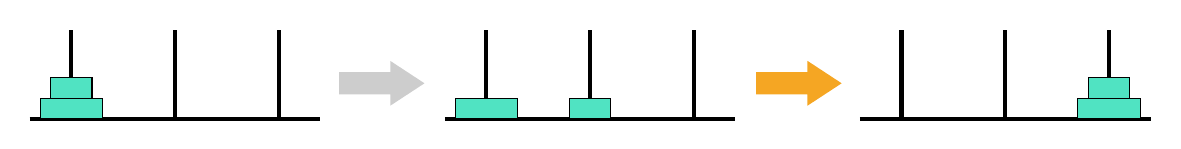
\begin{tikzpicture}[x=0.75pt,y=0.75pt,yscale=-1,xscale=1]
%uncomment if require: \path (0,300); %set diagram left start at 0, and has height of 300

%Straight Lines [id:da20128490011342937] 
\draw [line width=1.5]    (0,43) -- (140,43) ;
%Straight Lines [id:da6199160713043812] 
\draw [line width=1.5]    (20,43) -- (20,0) ;
%Straight Lines [id:da8216195699647504] 
\draw [line width=1.5]    (70,43) -- (70,0) ;
%Straight Lines [id:da5396733017684658] 
\draw [line width=1.5]    (120,43) -- (120,0) ;
%Shape: Rectangle [id:dp8201450749921013] 
\draw  [fill={rgb, 255:red, 80; green, 227; blue, 194 }  ,fill opacity=1 ] (10,23) -- (30,23) -- (30,33) -- (10,33) -- cycle ;
%Shape: Rectangle [id:dp2896614158424695] 
\draw  [fill={rgb, 255:red, 80; green, 227; blue, 194 }  ,fill opacity=1 ] (5,33) -- (35,33) -- (35,43) -- (5,43) -- cycle ;
%Straight Lines [id:da38074031093924554] 
\draw [line width=1.5]    (200,43) -- (340,43) ;
%Straight Lines [id:da17073098870278036] 
\draw [line width=1.5]    (220,43) -- (220,0) ;
%Straight Lines [id:da5016561498079584] 
\draw [line width=1.5]    (270,43) -- (270,0) ;
%Straight Lines [id:da39100060600554376] 
\draw [line width=1.5]    (320,43) -- (320,0) ;
%Shape: Rectangle [id:dp7482815217136263] 
\draw  [fill={rgb, 255:red, 80; green, 227; blue, 194 }  ,fill opacity=1 ] (260,33) -- (280,33) -- (280,43) -- (260,43) -- cycle ;
%Shape: Rectangle [id:dp7784470454205272] 
\draw  [fill={rgb, 255:red, 80; green, 227; blue, 194 }  ,fill opacity=1 ] (205,33) -- (235,33) -- (235,43) -- (205,43) -- cycle ;
%Straight Lines [id:da3236508180561881] 
\draw [line width=1.5]    (400,43) -- (540,43) ;
%Straight Lines [id:da9709328304324318] 
\draw [line width=1.5]    (420,43) -- (420,0) ;
%Straight Lines [id:da2363002999549213] 
\draw [line width=1.5]    (470,43) -- (470,0) ;
%Straight Lines [id:da13139163205712556] 
\draw [line width=1.5]    (520,43) -- (520,0) ;
%Shape: Rectangle [id:dp6159066559936051] 
\draw  [fill={rgb, 255:red, 80; green, 227; blue, 194 }  ,fill opacity=1 ] (510,23) -- (530,23) -- (530,33) -- (510,33) -- cycle ;
%Shape: Rectangle [id:dp34198986529751507] 
\draw  [fill={rgb, 255:red, 80; green, 227; blue, 194 }  ,fill opacity=1 ] (505,33) -- (535,33) -- (535,43) -- (505,43) -- cycle ;
%Right Arrow [id:dp770167769543662] 
\draw  [draw opacity=0][fill={rgb, 255:red, 155; green, 155; blue, 155 }  ,fill opacity=0.5 ] (149,20.4) -- (173.71,20.4) -- (173.71,15) -- (190.18,25.8) -- (173.71,36.59) -- (173.71,31.19) -- (149,31.19) -- cycle ;
%Right Arrow [id:dp8521060197848471] 
\draw  [draw opacity=0][fill={rgb, 255:red, 245; green, 166; blue, 35 }  ,fill opacity=1 ] (350,20.4) -- (374.71,20.4) -- (374.71,15) -- (391.18,25.8) -- (374.71,36.59) -- (374.71,31.19) -- (350,31.19) -- cycle ;




\end{tikzpicture}
    \caption{The solution of the Tower of Fibonacci with $n=2$ discs.}
\end{figure}

\begin{figure}[H]
    \centering
    

\tikzset{every picture/.style={line width=0.75pt}} %set default line width to 0.75pt        

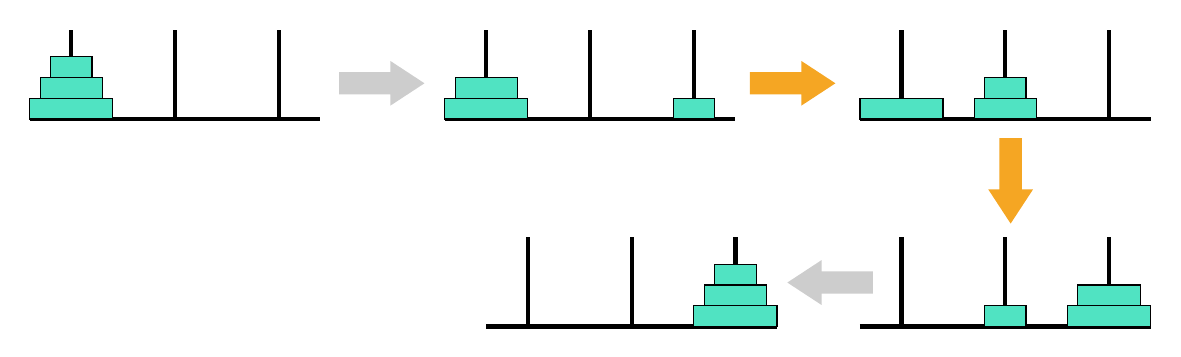
\begin{tikzpicture}[x=0.75pt,y=0.75pt,yscale=-1,xscale=1]
%uncomment if require: \path (0,300); %set diagram left start at 0, and has height of 300

%Straight Lines [id:da8303538154751591] 
\draw [line width=1.5]    (0,43) -- (140,43) ;
%Straight Lines [id:da44377290589200835] 
\draw [line width=1.5]    (20,43) -- (20,0) ;
%Straight Lines [id:da31239925834279325] 
\draw [line width=1.5]    (70,43) -- (70,0) ;
%Straight Lines [id:da04391756158348037] 
\draw [line width=1.5]    (120,43) -- (120,0) ;
%Shape: Rectangle [id:dp7875199976215352] 
\draw  [fill={rgb, 255:red, 80; green, 227; blue, 194 }  ,fill opacity=1 ] (10,13) -- (30,13) -- (30,23) -- (10,23) -- cycle ;
%Shape: Rectangle [id:dp5137168472398668] 
\draw  [fill={rgb, 255:red, 80; green, 227; blue, 194 }  ,fill opacity=1 ] (5,23) -- (35,23) -- (35,33) -- (5,33) -- cycle ;
%Shape: Rectangle [id:dp5712905937546608] 
\draw  [fill={rgb, 255:red, 80; green, 227; blue, 194 }  ,fill opacity=1 ] (0,33) -- (40,33) -- (40,43) -- (0,43) -- cycle ;
%Straight Lines [id:da34969225911400326] 
\draw [line width=1.5]    (200,43) -- (340,43) ;
%Straight Lines [id:da8901348300768355] 
\draw [line width=1.5]    (220,43) -- (220,0) ;
%Straight Lines [id:da003633824506256822] 
\draw [line width=1.5]    (270,43) -- (270,0) ;
%Straight Lines [id:da3099038211593088] 
\draw [line width=1.5]    (320,43) -- (320,0) ;
%Shape: Rectangle [id:dp853294561519496] 
\draw  [fill={rgb, 255:red, 80; green, 227; blue, 194 }  ,fill opacity=1 ] (310,33) -- (330,33) -- (330,43) -- (310,43) -- cycle ;
%Shape: Rectangle [id:dp6402799146261537] 
\draw  [fill={rgb, 255:red, 80; green, 227; blue, 194 }  ,fill opacity=1 ] (205,23) -- (235,23) -- (235,33) -- (205,33) -- cycle ;
%Shape: Rectangle [id:dp8924629231345207] 
\draw  [fill={rgb, 255:red, 80; green, 227; blue, 194 }  ,fill opacity=1 ] (200,33) -- (240,33) -- (240,43) -- (200,43) -- cycle ;
%Straight Lines [id:da804093067665645] 
\draw [line width=1.5]    (400,43) -- (540,43) ;
%Straight Lines [id:da9747644440126735] 
\draw [line width=1.5]    (420,43) -- (420,0) ;
%Straight Lines [id:da965021701225063] 
\draw [line width=1.5]    (470,43) -- (470,0) ;
%Straight Lines [id:da38823609700733286] 
\draw [line width=1.5]    (520,43) -- (520,0) ;
%Shape: Rectangle [id:dp309662324926796] 
\draw  [fill={rgb, 255:red, 80; green, 227; blue, 194 }  ,fill opacity=1 ] (460,23) -- (480,23) -- (480,33) -- (460,33) -- cycle ;
%Shape: Rectangle [id:dp866448991893723] 
\draw  [fill={rgb, 255:red, 80; green, 227; blue, 194 }  ,fill opacity=1 ] (455,33) -- (485,33) -- (485,43) -- (455,43) -- cycle ;
%Shape: Rectangle [id:dp4761201047419301] 
\draw  [fill={rgb, 255:red, 80; green, 227; blue, 194 }  ,fill opacity=1 ] (400,33) -- (440,33) -- (440,43) -- (400,43) -- cycle ;
%Straight Lines [id:da23259802146504427] 
\draw [line width=1.5]    (400,143) -- (540,143) ;
%Straight Lines [id:da5186458559134219] 
\draw [line width=1.5]    (420,143) -- (420,100) ;
%Straight Lines [id:da5855834682713619] 
\draw [line width=1.5]    (470,143) -- (470,100) ;
%Straight Lines [id:da5018356523168015] 
\draw [line width=1.5]    (520,143) -- (520,100) ;
%Shape: Rectangle [id:dp42151194739698905] 
\draw  [fill={rgb, 255:red, 80; green, 227; blue, 194 }  ,fill opacity=1 ] (460,133) -- (480,133) -- (480,143) -- (460,143) -- cycle ;
%Shape: Rectangle [id:dp6404422858687056] 
\draw  [fill={rgb, 255:red, 80; green, 227; blue, 194 }  ,fill opacity=1 ] (505,123) -- (535,123) -- (535,133) -- (505,133) -- cycle ;
%Shape: Rectangle [id:dp14892112371290667] 
\draw  [fill={rgb, 255:red, 80; green, 227; blue, 194 }  ,fill opacity=1 ] (500,133) -- (540,133) -- (540,143) -- (500,143) -- cycle ;
%Straight Lines [id:da8258744881158513] 
\draw [line width=1.5]    (220,143) -- (360,143) ;
%Straight Lines [id:da9176858810792492] 
\draw [line width=1.5]    (240,143) -- (240,100) ;
%Straight Lines [id:da05677154242854954] 
\draw [line width=1.5]    (290,143) -- (290,100) ;
%Straight Lines [id:da4712882771924096] 
\draw [line width=1.5]    (340,143) -- (340,100) ;
%Shape: Rectangle [id:dp7420825715378909] 
\draw  [fill={rgb, 255:red, 80; green, 227; blue, 194 }  ,fill opacity=1 ] (330,113) -- (350,113) -- (350,123) -- (330,123) -- cycle ;
%Shape: Rectangle [id:dp7326725119770061] 
\draw  [fill={rgb, 255:red, 80; green, 227; blue, 194 }  ,fill opacity=1 ] (325,123) -- (355,123) -- (355,133) -- (325,133) -- cycle ;
%Shape: Rectangle [id:dp44218831851720064] 
\draw  [fill={rgb, 255:red, 80; green, 227; blue, 194 }  ,fill opacity=1 ] (320,133) -- (360,133) -- (360,143) -- (320,143) -- cycle ;
%Right Arrow [id:dp584858819424027] 
\draw  [draw opacity=0][fill={rgb, 255:red, 155; green, 155; blue, 155 }  ,fill opacity=0.5 ] (149,20.4) -- (173.71,20.4) -- (173.71,15) -- (190.18,25.8) -- (173.71,36.59) -- (173.71,31.19) -- (149,31.19) -- cycle ;
%Right Arrow [id:dp6955937550375395] 
\draw  [draw opacity=0][fill={rgb, 255:red, 245; green, 166; blue, 35 }  ,fill opacity=1 ] (347,20.4) -- (371.71,20.4) -- (371.71,15) -- (388.18,25.8) -- (371.71,36.59) -- (371.71,31.19) -- (347,31.19) -- cycle ;
%Right Arrow [id:dp7728167634857226] 
\draw  [draw opacity=0][fill={rgb, 255:red, 155; green, 155; blue, 155 }  ,fill opacity=0.5 ] (406.18,127.19) -- (381.47,127.19) -- (381.47,132.59) -- (365,121.8) -- (381.47,111) -- (381.47,116.4) -- (406.18,116.4) -- cycle ;
%Right Arrow [id:dp16004852915276047] 
\draw  [draw opacity=0][fill={rgb, 255:red, 245; green, 166; blue, 35 }  ,fill opacity=1 ] (477.99,52.2) -- (477.99,76.91) -- (483.39,76.91) -- (472.59,93.39) -- (461.8,76.91) -- (467.19,76.91) -- (467.19,52.2) -- cycle ;




\end{tikzpicture}
    \caption{The solution of the Tower of Fibonacci with $n=3$ discs.}
\end{figure}


\subsection{Tower of Lucas}
\begin{figure}[H]
    \centering
    

\tikzset{every picture/.style={line width=0.75pt}} %set default line width to 0.75pt        

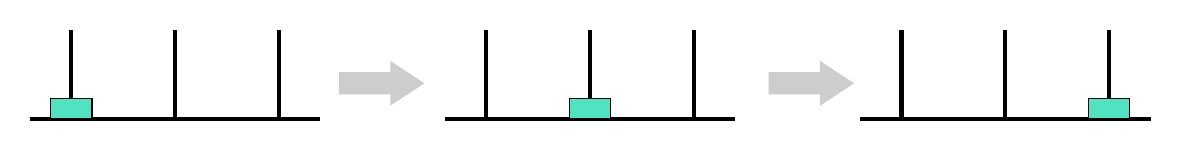
\begin{tikzpicture}[x=0.75pt,y=0.75pt,yscale=-1,xscale=1]
%uncomment if require: \path (0,300); %set diagram left start at 0, and has height of 300

%Straight Lines [id:da44397547129105375] 
\draw [line width=1.5]    (0,43) -- (140,43) ;
%Straight Lines [id:da4645503646398441] 
\draw [line width=1.5]    (20,43) -- (20,0) ;
%Straight Lines [id:da18570484631161044] 
\draw [line width=1.5]    (70,43) -- (70,0) ;
%Straight Lines [id:da24900095483501095] 
\draw [line width=1.5]    (120,43) -- (120,0) ;
%Shape: Rectangle [id:dp8474340181669155] 
\draw  [fill={rgb, 255:red, 80; green, 227; blue, 194 }  ,fill opacity=1 ] (10,33) -- (30,33) -- (30,43) -- (10,43) -- cycle ;
%Straight Lines [id:da7189985957808207] 
\draw [line width=1.5]    (400,43) -- (540,43) ;
%Straight Lines [id:da9421870195405853] 
\draw [line width=1.5]    (420,43) -- (420,0) ;
%Straight Lines [id:da4273644854629841] 
\draw [line width=1.5]    (470,43) -- (470,0) ;
%Straight Lines [id:da7660398894506095] 
\draw [line width=1.5]    (520,43) -- (520,0) ;
%Shape: Rectangle [id:dp22186357606673335] 
\draw  [fill={rgb, 255:red, 80; green, 227; blue, 194 }  ,fill opacity=1 ] (510,33) -- (530,33) -- (530,43) -- (510,43) -- cycle ;
%Right Arrow [id:dp2775003592778411] 
\draw  [draw opacity=0][fill={rgb, 255:red, 155; green, 155; blue, 155 }  ,fill opacity=0.5 ] (149,20.4) -- (173.71,20.4) -- (173.71,15) -- (190.18,25.8) -- (173.71,36.59) -- (173.71,31.19) -- (149,31.19) -- cycle ;
%Straight Lines [id:da8318825611109566] 
\draw [line width=1.5]    (200,43) -- (340,43) ;
%Straight Lines [id:da38588092673028096] 
\draw [line width=1.5]    (220,43) -- (220,0) ;
%Straight Lines [id:da31788455293266815] 
\draw [line width=1.5]    (270,43) -- (270,0) ;
%Straight Lines [id:da23303223029131237] 
\draw [line width=1.5]    (320,43) -- (320,0) ;
%Shape: Rectangle [id:dp4086300145485118] 
\draw  [fill={rgb, 255:red, 80; green, 227; blue, 194 }  ,fill opacity=1 ] (260,33) -- (280,33) -- (280,43) -- (260,43) -- cycle ;
%Right Arrow [id:dp667691844561485] 
\draw  [draw opacity=0][fill={rgb, 255:red, 155; green, 155; blue, 155 }  ,fill opacity=0.5 ] (356,20.4) -- (380.71,20.4) -- (380.71,15) -- (397.18,25.8) -- (380.71,36.59) -- (380.71,31.19) -- (356,31.19) -- cycle ;




\end{tikzpicture}
    \caption{The solution of the Tower of Lucas with $n=1$ discs.}
\end{figure}

\begin{figure}[H]
    \centering
    

\tikzset{every picture/.style={line width=0.75pt}} %set default line width to 0.75pt        

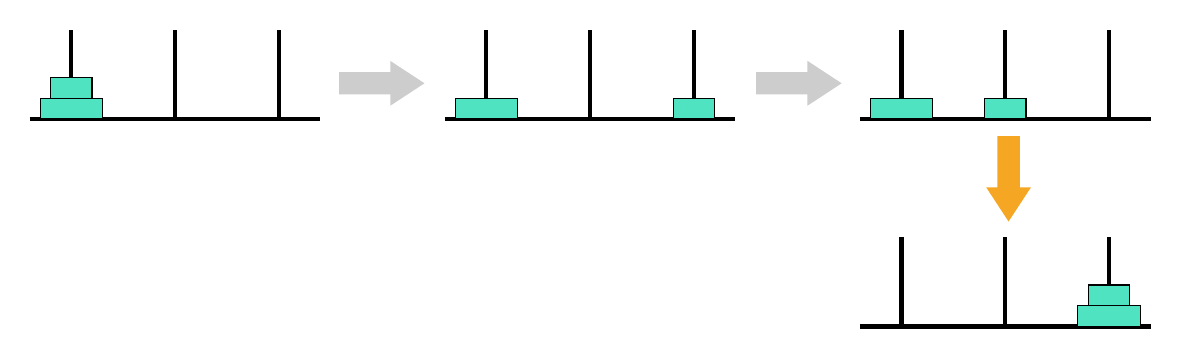
\begin{tikzpicture}[x=0.75pt,y=0.75pt,yscale=-1,xscale=1]
%uncomment if require: \path (0,300); %set diagram left start at 0, and has height of 300

%Straight Lines [id:da13726702625512988] 
\draw [line width=1.5]    (0,43) -- (140,43) ;
%Straight Lines [id:da15360582919452215] 
\draw [line width=1.5]    (20,43) -- (20,0) ;
%Straight Lines [id:da6738920998567135] 
\draw [line width=1.5]    (70,43) -- (70,0) ;
%Straight Lines [id:da7724994784589692] 
\draw [line width=1.5]    (120,43) -- (120,0) ;
%Shape: Rectangle [id:dp6321704129575834] 
\draw  [fill={rgb, 255:red, 80; green, 227; blue, 194 }  ,fill opacity=1 ] (10,23) -- (30,23) -- (30,33) -- (10,33) -- cycle ;
%Shape: Rectangle [id:dp9032710209350665] 
\draw  [fill={rgb, 255:red, 80; green, 227; blue, 194 }  ,fill opacity=1 ] (5,33) -- (35,33) -- (35,43) -- (5,43) -- cycle ;
%Straight Lines [id:da8114672346662017] 
\draw [line width=1.5]    (200,43) -- (340,43) ;
%Straight Lines [id:da5639432337449439] 
\draw [line width=1.5]    (220,43) -- (220,0) ;
%Straight Lines [id:da946790537568112] 
\draw [line width=1.5]    (270,43) -- (270,0) ;
%Straight Lines [id:da9270288420079429] 
\draw [line width=1.5]    (320,43) -- (320,0) ;
%Shape: Rectangle [id:dp37679845060629513] 
\draw  [fill={rgb, 255:red, 80; green, 227; blue, 194 }  ,fill opacity=1 ] (310,33) -- (330,33) -- (330,43) -- (310,43) -- cycle ;
%Shape: Rectangle [id:dp2372445695079224] 
\draw  [fill={rgb, 255:red, 80; green, 227; blue, 194 }  ,fill opacity=1 ] (205,33) -- (235,33) -- (235,43) -- (205,43) -- cycle ;
%Straight Lines [id:da07903448163852556] 
\draw [line width=1.5]    (400,43) -- (540,43) ;
%Straight Lines [id:da43632403351772964] 
\draw [line width=1.5]    (420,43) -- (420,0) ;
%Straight Lines [id:da2704456144468119] 
\draw [line width=1.5]    (470,43) -- (470,0) ;
%Straight Lines [id:da6426435178388965] 
\draw [line width=1.5]    (520,43) -- (520,0) ;
%Shape: Rectangle [id:dp8070069771053439] 
\draw  [fill={rgb, 255:red, 80; green, 227; blue, 194 }  ,fill opacity=1 ] (460,33) -- (480,33) -- (480,43) -- (460,43) -- cycle ;
%Shape: Rectangle [id:dp18772749326779192] 
\draw  [fill={rgb, 255:red, 80; green, 227; blue, 194 }  ,fill opacity=1 ] (405,33) -- (435,33) -- (435,43) -- (405,43) -- cycle ;
%Right Arrow [id:dp5241948928000351] 
\draw  [draw opacity=0][fill={rgb, 255:red, 155; green, 155; blue, 155 }  ,fill opacity=0.5 ] (149,20.4) -- (173.71,20.4) -- (173.71,15) -- (190.18,25.8) -- (173.71,36.59) -- (173.71,31.19) -- (149,31.19) -- cycle ;
%Right Arrow [id:dp5104462153168119] 
\draw  [draw opacity=0][fill={rgb, 255:red, 155; green, 155; blue, 155 }  ,fill opacity=0.5 ] (350,20.4) -- (374.71,20.4) -- (374.71,15) -- (391.18,25.8) -- (374.71,36.59) -- (374.71,31.19) -- (350,31.19) -- cycle ;
%Straight Lines [id:da49228015662387725] 
\draw [line width=1.5]    (400,143) -- (540,143) ;
%Straight Lines [id:da7861217924177282] 
\draw [line width=1.5]    (420,143) -- (420,100) ;
%Straight Lines [id:da19859236755289955] 
\draw [line width=1.5]    (470,143) -- (470,100) ;
%Straight Lines [id:da7443410481299351] 
\draw [line width=1.5]    (520,143) -- (520,100) ;
%Shape: Rectangle [id:dp1489451725407407] 
\draw  [fill={rgb, 255:red, 80; green, 227; blue, 194 }  ,fill opacity=1 ] (510,123) -- (530,123) -- (530,133) -- (510,133) -- cycle ;
%Shape: Rectangle [id:dp8784844243354075] 
\draw  [fill={rgb, 255:red, 80; green, 227; blue, 194 }  ,fill opacity=1 ] (505,133) -- (535,133) -- (535,143) -- (505,143) -- cycle ;
%Right Arrow [id:dp2702152662492525] 
\draw  [draw opacity=0][fill={rgb, 255:red, 245; green, 166; blue, 35 }  ,fill opacity=1 ] (476.99,51.2) -- (476.99,75.91) -- (482.39,75.91) -- (471.59,92.39) -- (460.8,75.91) -- (466.19,75.91) -- (466.19,51.2) -- cycle ;




\end{tikzpicture}
    \caption{The solution of the Tower of Lucas with $n=2$ discs.}
\end{figure}

\begin{figure}[H]
    \centering
    

\tikzset{every picture/.style={line width=0.75pt}} %set default line width to 0.75pt        

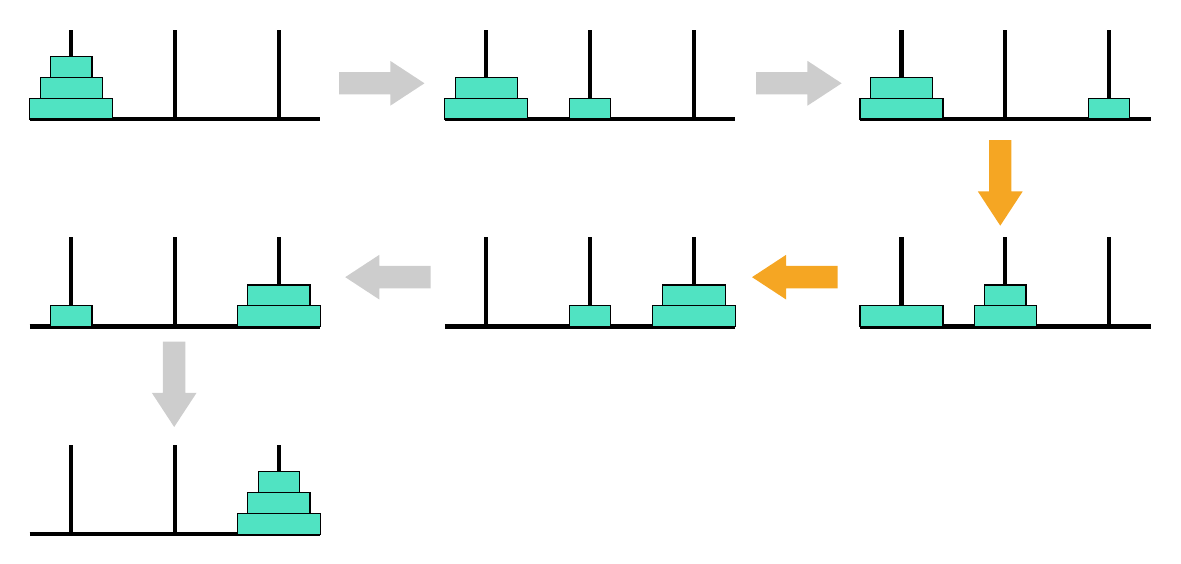
\begin{tikzpicture}[x=0.75pt,y=0.75pt,yscale=-1,xscale=1]
%uncomment if require: \path (0,300); %set diagram left start at 0, and has height of 300

%Straight Lines [id:da8025082395649901] 
\draw [line width=1.5]    (0,43) -- (140,43) ;
%Straight Lines [id:da7454643049605156] 
\draw [line width=1.5]    (20,43) -- (20,0) ;
%Straight Lines [id:da9870306919504184] 
\draw [line width=1.5]    (70,43) -- (70,0) ;
%Straight Lines [id:da7982234424576593] 
\draw [line width=1.5]    (120,43) -- (120,0) ;
%Shape: Rectangle [id:dp31308727004250536] 
\draw  [fill={rgb, 255:red, 80; green, 227; blue, 194 }  ,fill opacity=1 ] (10,13) -- (30,13) -- (30,23) -- (10,23) -- cycle ;
%Shape: Rectangle [id:dp3777412161248892] 
\draw  [fill={rgb, 255:red, 80; green, 227; blue, 194 }  ,fill opacity=1 ] (5,23) -- (35,23) -- (35,33) -- (5,33) -- cycle ;
%Shape: Rectangle [id:dp7763953163886761] 
\draw  [fill={rgb, 255:red, 80; green, 227; blue, 194 }  ,fill opacity=1 ] (0,33) -- (40,33) -- (40,43) -- (0,43) -- cycle ;
%Straight Lines [id:da6272660525985647] 
\draw [line width=1.5]    (200,43) -- (340,43) ;
%Straight Lines [id:da5081746449047639] 
\draw [line width=1.5]    (220,43) -- (220,0) ;
%Straight Lines [id:da2165918471753694] 
\draw [line width=1.5]    (270,43) -- (270,0) ;
%Straight Lines [id:da37427815250463214] 
\draw [line width=1.5]    (320,43) -- (320,0) ;
%Shape: Rectangle [id:dp8232086571512724] 
\draw  [fill={rgb, 255:red, 80; green, 227; blue, 194 }  ,fill opacity=1 ] (260,33) -- (280,33) -- (280,43) -- (260,43) -- cycle ;
%Shape: Rectangle [id:dp8644420281655714] 
\draw  [fill={rgb, 255:red, 80; green, 227; blue, 194 }  ,fill opacity=1 ] (205,23) -- (235,23) -- (235,33) -- (205,33) -- cycle ;
%Shape: Rectangle [id:dp4691112599802305] 
\draw  [fill={rgb, 255:red, 80; green, 227; blue, 194 }  ,fill opacity=1 ] (200,33) -- (240,33) -- (240,43) -- (200,43) -- cycle ;
%Straight Lines [id:da9973522843967422] 
\draw [line width=1.5]    (400,43) -- (540,43) ;
%Straight Lines [id:da28667125764852375] 
\draw [line width=1.5]    (420,43) -- (420,0) ;
%Straight Lines [id:da381214361474431] 
\draw [line width=1.5]    (470,43) -- (470,0) ;
%Straight Lines [id:da9860623872856136] 
\draw [line width=1.5]    (520,43) -- (520,0) ;
%Shape: Rectangle [id:dp16695186089193936] 
\draw  [fill={rgb, 255:red, 80; green, 227; blue, 194 }  ,fill opacity=1 ] (510,33) -- (530,33) -- (530,43) -- (510,43) -- cycle ;
%Shape: Rectangle [id:dp014735201879446658] 
\draw  [fill={rgb, 255:red, 80; green, 227; blue, 194 }  ,fill opacity=1 ] (405,23) -- (435,23) -- (435,33) -- (405,33) -- cycle ;
%Shape: Rectangle [id:dp22542966194511638] 
\draw  [fill={rgb, 255:red, 80; green, 227; blue, 194 }  ,fill opacity=1 ] (400,33) -- (440,33) -- (440,43) -- (400,43) -- cycle ;
%Right Arrow [id:dp817845334848694] 
\draw  [draw opacity=0][fill={rgb, 255:red, 155; green, 155; blue, 155 }  ,fill opacity=0.5 ] (149,20.4) -- (173.71,20.4) -- (173.71,15) -- (190.18,25.8) -- (173.71,36.59) -- (173.71,31.19) -- (149,31.19) -- cycle ;
%Right Arrow [id:dp6018982469067375] 
\draw  [draw opacity=0][fill={rgb, 255:red, 155; green, 155; blue, 155 }  ,fill opacity=0.5 ] (350,20.4) -- (374.71,20.4) -- (374.71,15) -- (391.18,25.8) -- (374.71,36.59) -- (374.71,31.19) -- (350,31.19) -- cycle ;
%Straight Lines [id:da13821415983405227] 
\draw [line width=1.5]    (400,143) -- (540,143) ;
%Straight Lines [id:da5216664359899352] 
\draw [line width=1.5]    (420,143) -- (420,100) ;
%Straight Lines [id:da44716880682990956] 
\draw [line width=1.5]    (470,143) -- (470,100) ;
%Straight Lines [id:da4101697946658833] 
\draw [line width=1.5]    (520,143) -- (520,100) ;
%Shape: Rectangle [id:dp3567554057464952] 
\draw  [fill={rgb, 255:red, 80; green, 227; blue, 194 }  ,fill opacity=1 ] (460,123) -- (480,123) -- (480,133) -- (460,133) -- cycle ;
%Shape: Rectangle [id:dp12678576360054183] 
\draw  [fill={rgb, 255:red, 80; green, 227; blue, 194 }  ,fill opacity=1 ] (455,133) -- (485,133) -- (485,143) -- (455,143) -- cycle ;
%Shape: Rectangle [id:dp4776717430974402] 
\draw  [fill={rgb, 255:red, 80; green, 227; blue, 194 }  ,fill opacity=1 ] (400,133) -- (440,133) -- (440,143) -- (400,143) -- cycle ;
%Straight Lines [id:da9914930648809162] 
\draw [line width=1.5]    (200,143) -- (340,143) ;
%Straight Lines [id:da25229761332615785] 
\draw [line width=1.5]    (220,143) -- (220,100) ;
%Straight Lines [id:da40305779614297244] 
\draw [line width=1.5]    (270,143) -- (270,100) ;
%Straight Lines [id:da9846311638402929] 
\draw [line width=1.5]    (320,143) -- (320,100) ;
%Shape: Rectangle [id:dp38605928137718815] 
\draw  [fill={rgb, 255:red, 80; green, 227; blue, 194 }  ,fill opacity=1 ] (260,133) -- (280,133) -- (280,143) -- (260,143) -- cycle ;
%Shape: Rectangle [id:dp690534374681401] 
\draw  [fill={rgb, 255:red, 80; green, 227; blue, 194 }  ,fill opacity=1 ] (305,123) -- (335,123) -- (335,133) -- (305,133) -- cycle ;
%Shape: Rectangle [id:dp5647982668686782] 
\draw  [fill={rgb, 255:red, 80; green, 227; blue, 194 }  ,fill opacity=1 ] (300,133) -- (340,133) -- (340,143) -- (300,143) -- cycle ;
%Straight Lines [id:da7047084068028082] 
\draw [line width=1.5]    (0,143) -- (140,143) ;
%Straight Lines [id:da40713814496755685] 
\draw [line width=1.5]    (20,143) -- (20,100) ;
%Straight Lines [id:da7435733536391158] 
\draw [line width=1.5]    (70,143) -- (70,100) ;
%Straight Lines [id:da00865886562674878] 
\draw [line width=1.5]    (120,143) -- (120,100) ;
%Shape: Rectangle [id:dp8916733675456492] 
\draw  [fill={rgb, 255:red, 80; green, 227; blue, 194 }  ,fill opacity=1 ] (10,133) -- (30,133) -- (30,143) -- (10,143) -- cycle ;
%Shape: Rectangle [id:dp15563711600479446] 
\draw  [fill={rgb, 255:red, 80; green, 227; blue, 194 }  ,fill opacity=1 ] (105,123) -- (135,123) -- (135,133) -- (105,133) -- cycle ;
%Shape: Rectangle [id:dp7151630467413674] 
\draw  [fill={rgb, 255:red, 80; green, 227; blue, 194 }  ,fill opacity=1 ] (100,133) -- (140,133) -- (140,143) -- (100,143) -- cycle ;
%Straight Lines [id:da791380685908035] 
\draw [line width=1.5]    (0,243) -- (140,243) ;
%Straight Lines [id:da9627624209763874] 
\draw [line width=1.5]    (20,243) -- (20,200) ;
%Straight Lines [id:da5706344465533184] 
\draw [line width=1.5]    (70,243) -- (70,200) ;
%Straight Lines [id:da6272022449172838] 
\draw [line width=1.5]    (120,243) -- (120,200) ;
%Shape: Rectangle [id:dp7172186994557044] 
\draw  [fill={rgb, 255:red, 80; green, 227; blue, 194 }  ,fill opacity=1 ] (110,213) -- (130,213) -- (130,223) -- (110,223) -- cycle ;
%Shape: Rectangle [id:dp10548139179292937] 
\draw  [fill={rgb, 255:red, 80; green, 227; blue, 194 }  ,fill opacity=1 ] (105,223) -- (135,223) -- (135,233) -- (105,233) -- cycle ;
%Shape: Rectangle [id:dp6761200435231796] 
\draw  [fill={rgb, 255:red, 80; green, 227; blue, 194 }  ,fill opacity=1 ] (100,233) -- (140,233) -- (140,243) -- (100,243) -- cycle ;
%Right Arrow [id:dp24211937744475276] 
\draw  [draw opacity=0][fill={rgb, 255:red, 245; green, 166; blue, 35 }  ,fill opacity=1 ] (472.99,53.2) -- (472.99,77.91) -- (478.39,77.91) -- (467.59,94.39) -- (456.8,77.91) -- (462.19,77.91) -- (462.19,53.2) -- cycle ;
%Right Arrow [id:dp644145870601811] 
\draw  [draw opacity=0][fill={rgb, 255:red, 155; green, 155; blue, 155 }  ,fill opacity=0.5 ] (74.99,150.2) -- (74.99,174.91) -- (80.39,174.91) -- (69.59,191.39) -- (58.8,174.91) -- (64.19,174.91) -- (64.19,150.2) -- cycle ;
%Right Arrow [id:dp05615444085078236] 
\draw  [draw opacity=0][fill={rgb, 255:red, 245; green, 166; blue, 35 }  ,fill opacity=1 ] (389.18,124.6) -- (364.47,124.6) -- (364.47,130) -- (348,119.2) -- (364.47,108.41) -- (364.47,113.81) -- (389.18,113.81) -- cycle ;
%Right Arrow [id:dp6272677230050907] 
\draw  [draw opacity=0][fill={rgb, 255:red, 155; green, 155; blue, 155 }  ,fill opacity=0.5 ] (193.18,124.6) -- (168.47,124.6) -- (168.47,130) -- (152,119.2) -- (168.47,108.41) -- (168.47,113.81) -- (193.18,113.81) -- cycle ;




\end{tikzpicture}
    \caption{The solution of the Tower of Lucas with $n=3$ discs.}
\end{figure}


\subsection{Tower of Jacobsthal}
\begin{figure}[H]
    \centering
    

\tikzset{every picture/.style={line width=0.75pt}} %set default line width to 0.75pt        

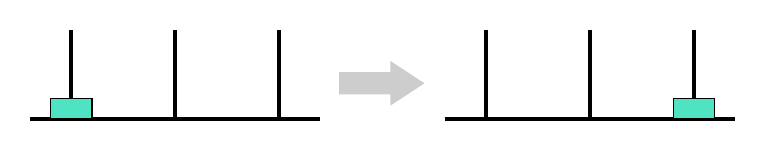
\begin{tikzpicture}[x=0.75pt,y=0.75pt,yscale=-1,xscale=1]
%uncomment if require: \path (0,387); %set diagram left start at 0, and has height of 387

%Straight Lines [id:da40902814921476005] 
\draw [line width=1.5]    (0,43) -- (140,43) ;
%Straight Lines [id:da32687008830530373] 
\draw [line width=1.5]    (20,43) -- (20,0) ;
%Straight Lines [id:da3172525661879657] 
\draw [line width=1.5]    (70,43) -- (70,0) ;
%Straight Lines [id:da3724427659815115] 
\draw [line width=1.5]    (120,43) -- (120,0) ;
%Shape: Rectangle [id:dp12926306550885913] 
\draw  [fill={rgb, 255:red, 80; green, 227; blue, 194 }  ,fill opacity=1 ] (10,33) -- (30,33) -- (30,43) -- (10,43) -- cycle ;
%Straight Lines [id:da944371051878028] 
\draw [line width=1.5]    (200,43) -- (340,43) ;
%Straight Lines [id:da5623860802403418] 
\draw [line width=1.5]    (220,43) -- (220,0) ;
%Straight Lines [id:da9847294698370319] 
\draw [line width=1.5]    (270,43) -- (270,0) ;
%Straight Lines [id:da7330741622812829] 
\draw [line width=1.5]    (320,43) -- (320,0) ;
%Shape: Rectangle [id:dp6766108174560563] 
\draw  [fill={rgb, 255:red, 80; green, 227; blue, 194 }  ,fill opacity=1 ] (310,33) -- (330,33) -- (330,43) -- (310,43) -- cycle ;
%Right Arrow [id:dp9017051385213559] 
\draw  [draw opacity=0][fill={rgb, 255:red, 155; green, 155; blue, 155 }  ,fill opacity=0.5 ] (149,20.4) -- (173.71,20.4) -- (173.71,15) -- (190.18,25.8) -- (173.71,36.59) -- (173.71,31.19) -- (149,31.19) -- cycle ;




\end{tikzpicture}
    \caption{The solution of the Tower of Jacobsthal with $n=1$ discs.}
\end{figure}

\begin{figure}[H]
    \centering
    

\tikzset{every picture/.style={line width=0.75pt}} %set default line width to 0.75pt        

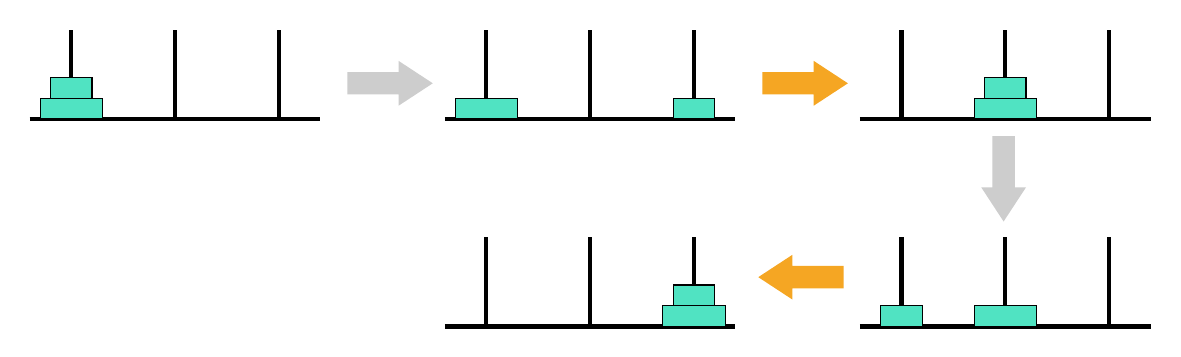
\begin{tikzpicture}[x=0.75pt,y=0.75pt,yscale=-1,xscale=1]
%uncomment if require: \path (0,300); %set diagram left start at 0, and has height of 300

%Straight Lines [id:da06505587060313123] 
\draw [line width=1.5]    (0,43) -- (140,43) ;
%Straight Lines [id:da8053950125861622] 
\draw [line width=1.5]    (20,43) -- (20,0) ;
%Straight Lines [id:da9817162928383374] 
\draw [line width=1.5]    (70,43) -- (70,0) ;
%Straight Lines [id:da2637271243076511] 
\draw [line width=1.5]    (120,43) -- (120,0) ;
%Shape: Rectangle [id:dp45068261565381307] 
\draw  [fill={rgb, 255:red, 80; green, 227; blue, 194 }  ,fill opacity=1 ] (10,23) -- (30,23) -- (30,33) -- (10,33) -- cycle ;
%Shape: Rectangle [id:dp9452534621237343] 
\draw  [fill={rgb, 255:red, 80; green, 227; blue, 194 }  ,fill opacity=1 ] (5,33) -- (35,33) -- (35,43) -- (5,43) -- cycle ;
%Straight Lines [id:da9256302717981051] 
\draw [line width=1.5]    (200,43) -- (340,43) ;
%Straight Lines [id:da20820143387913181] 
\draw [line width=1.5]    (220,43) -- (220,0) ;
%Straight Lines [id:da6074693511361262] 
\draw [line width=1.5]    (270,43) -- (270,0) ;
%Straight Lines [id:da35441541134250265] 
\draw [line width=1.5]    (320,43) -- (320,0) ;
%Shape: Rectangle [id:dp18246816823318723] 
\draw  [fill={rgb, 255:red, 80; green, 227; blue, 194 }  ,fill opacity=1 ] (310,33) -- (330,33) -- (330,43) -- (310,43) -- cycle ;
%Shape: Rectangle [id:dp6722986512308291] 
\draw  [fill={rgb, 255:red, 80; green, 227; blue, 194 }  ,fill opacity=1 ] (205,33) -- (235,33) -- (235,43) -- (205,43) -- cycle ;
%Straight Lines [id:da5955193495938234] 
\draw [line width=1.5]    (400,43) -- (540,43) ;
%Straight Lines [id:da2614963125190579] 
\draw [line width=1.5]    (420,43) -- (420,0) ;
%Straight Lines [id:da9595390777807311] 
\draw [line width=1.5]    (470,43) -- (470,0) ;
%Straight Lines [id:da9842508196064819] 
\draw [line width=1.5]    (520,43) -- (520,0) ;
%Shape: Rectangle [id:dp4043741719043581] 
\draw  [fill={rgb, 255:red, 80; green, 227; blue, 194 }  ,fill opacity=1 ] (460,23) -- (480,23) -- (480,33) -- (460,33) -- cycle ;
%Shape: Rectangle [id:dp7965103795770059] 
\draw  [fill={rgb, 255:red, 80; green, 227; blue, 194 }  ,fill opacity=1 ] (455,33) -- (485,33) -- (485,43) -- (455,43) -- cycle ;
%Straight Lines [id:da7664880125291995] 
\draw [line width=1.5]    (400,143) -- (540,143) ;
%Straight Lines [id:da8833936904388993] 
\draw [line width=1.5]    (420,143) -- (420,100) ;
%Straight Lines [id:da4102807413267129] 
\draw [line width=1.5]    (470,143) -- (470,100) ;
%Straight Lines [id:da10388059249374448] 
\draw [line width=1.5]    (520,143) -- (520,100) ;
%Shape: Rectangle [id:dp8079286503117589] 
\draw  [fill={rgb, 255:red, 80; green, 227; blue, 194 }  ,fill opacity=1 ] (410,133) -- (430,133) -- (430,143) -- (410,143) -- cycle ;
%Shape: Rectangle [id:dp9265435009476464] 
\draw  [fill={rgb, 255:red, 80; green, 227; blue, 194 }  ,fill opacity=1 ] (455,133) -- (485,133) -- (485,143) -- (455,143) -- cycle ;
%Straight Lines [id:da8623276338120203] 
\draw [line width=1.5]    (200,143) -- (340,143) ;
%Straight Lines [id:da06733148145525769] 
\draw [line width=1.5]    (220,143) -- (220,100) ;
%Straight Lines [id:da9288180973946829] 
\draw [line width=1.5]    (270,143) -- (270,100) ;
%Straight Lines [id:da5582304114403003] 
\draw [line width=1.5]    (320,143) -- (320,100) ;
%Shape: Rectangle [id:dp2664593640250392] 
\draw  [fill={rgb, 255:red, 80; green, 227; blue, 194 }  ,fill opacity=1 ] (310,123) -- (330,123) -- (330,133) -- (310,133) -- cycle ;
%Shape: Rectangle [id:dp16047488329441784] 
\draw  [fill={rgb, 255:red, 80; green, 227; blue, 194 }  ,fill opacity=1 ] (305,133) -- (335,133) -- (335,143) -- (305,143) -- cycle ;
%Right Arrow [id:dp6888341943746252] 
\draw  [draw opacity=0][fill={rgb, 255:red, 155; green, 155; blue, 155 }  ,fill opacity=0.5 ] (153,20.4) -- (177.71,20.4) -- (177.71,15) -- (194.18,25.8) -- (177.71,36.59) -- (177.71,31.19) -- (153,31.19) -- cycle ;
%Right Arrow [id:dp6032229542009344] 
\draw  [draw opacity=0][fill={rgb, 255:red, 245; green, 166; blue, 35 }  ,fill opacity=1 ] (353,20.4) -- (377.71,20.4) -- (377.71,15) -- (394.18,25.8) -- (377.71,36.59) -- (377.71,31.19) -- (353,31.19) -- cycle ;
%Right Arrow [id:dp40845900609658026] 
\draw  [draw opacity=0][fill={rgb, 255:red, 155; green, 155; blue, 155 }  ,fill opacity=0.5 ] (474.6,51.2) -- (474.6,75.91) -- (480,75.91) -- (469.2,92.39) -- (458.41,75.91) -- (463.81,75.91) -- (463.81,51.2) -- cycle ;
%Right Arrow [id:dp5367843345641361] 
\draw  [draw opacity=0][fill={rgb, 255:red, 245; green, 166; blue, 35 }  ,fill opacity=1 ] (392.18,124.6) -- (367.47,124.6) -- (367.47,130) -- (351,119.2) -- (367.47,108.41) -- (367.47,113.81) -- (392.18,113.81) -- cycle ;




\end{tikzpicture}
    \caption{The solution of the Tower of Jacobsthal with $n=2$ discs.}
\end{figure}

\begin{figure}[H]
    \centering
    

\tikzset{every picture/.style={line width=0.75pt}} %set default line width to 0.75pt        

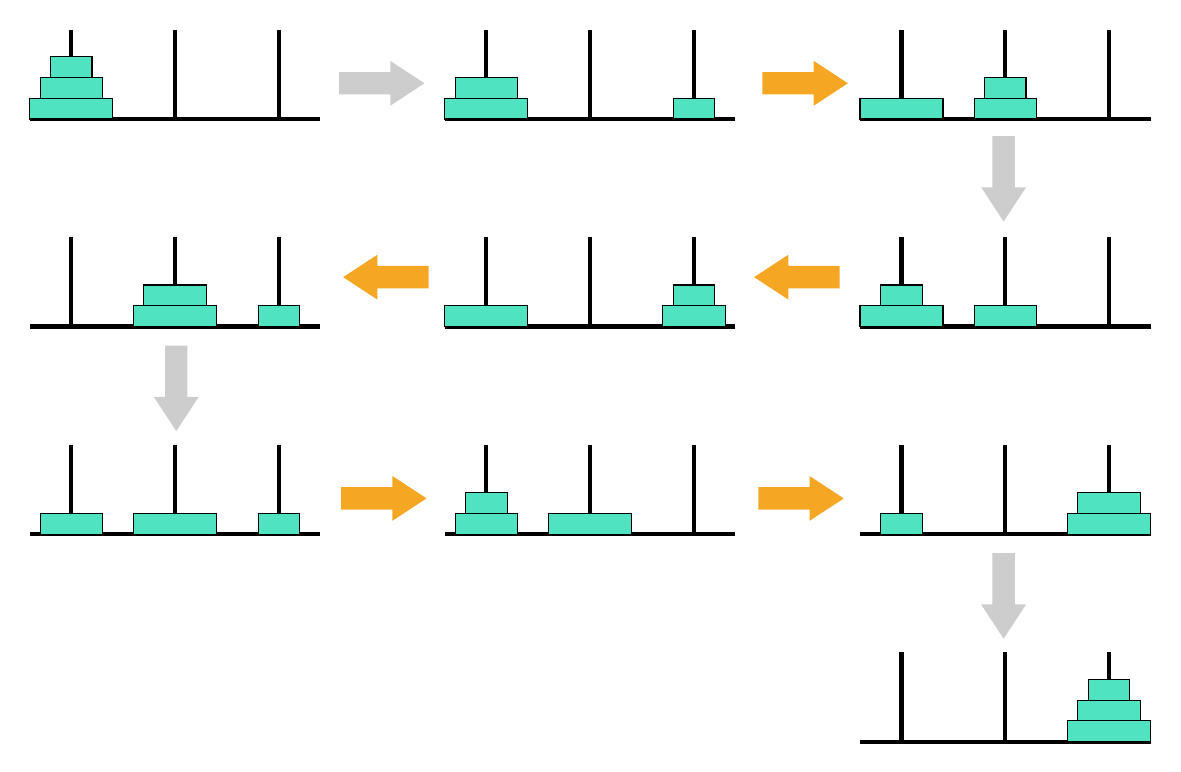
\begin{tikzpicture}[x=0.75pt,y=0.75pt,yscale=-1,xscale=1]
%uncomment if require: \path (0,387); %set diagram left start at 0, and has height of 387

%Straight Lines [id:da5159627573586094] 
\draw [line width=1.5]    (0,43) -- (140,43) ;
%Straight Lines [id:da34229017769899106] 
\draw [line width=1.5]    (20,43) -- (20,0) ;
%Straight Lines [id:da29640312136152414] 
\draw [line width=1.5]    (70,43) -- (70,0) ;
%Straight Lines [id:da45339481919819424] 
\draw [line width=1.5]    (120,43) -- (120,0) ;
%Shape: Rectangle [id:dp7399137628278751] 
\draw  [fill={rgb, 255:red, 80; green, 227; blue, 194 }  ,fill opacity=1 ] (10,13) -- (30,13) -- (30,23) -- (10,23) -- cycle ;
%Shape: Rectangle [id:dp15007793114766765] 
\draw  [fill={rgb, 255:red, 80; green, 227; blue, 194 }  ,fill opacity=1 ] (5,23) -- (35,23) -- (35,33) -- (5,33) -- cycle ;
%Shape: Rectangle [id:dp6311986719211768] 
\draw  [fill={rgb, 255:red, 80; green, 227; blue, 194 }  ,fill opacity=1 ] (0,33) -- (40,33) -- (40,43) -- (0,43) -- cycle ;
%Right Arrow [id:dp0780542586119517] 
\draw  [draw opacity=0][fill={rgb, 255:red, 155; green, 155; blue, 155 }  ,fill opacity=0.5 ] (149,20.4) -- (173.71,20.4) -- (173.71,15) -- (190.18,25.8) -- (173.71,36.59) -- (173.71,31.19) -- (149,31.19) -- cycle ;
%Straight Lines [id:da5240806584608748] 
\draw [line width=1.5]    (200,43) -- (340,43) ;
%Straight Lines [id:da6742579011717849] 
\draw [line width=1.5]    (220,43) -- (220,0) ;
%Straight Lines [id:da504219254308923] 
\draw [line width=1.5]    (270,43) -- (270,0) ;
%Straight Lines [id:da13913906276526578] 
\draw [line width=1.5]    (320,43) -- (320,0) ;
%Shape: Rectangle [id:dp39573893312883635] 
\draw  [fill={rgb, 255:red, 80; green, 227; blue, 194 }  ,fill opacity=1 ] (310,33) -- (330,33) -- (330,43) -- (310,43) -- cycle ;
%Shape: Rectangle [id:dp009602340238106466] 
\draw  [fill={rgb, 255:red, 80; green, 227; blue, 194 }  ,fill opacity=1 ] (205,23) -- (235,23) -- (235,33) -- (205,33) -- cycle ;
%Shape: Rectangle [id:dp4895424965815398] 
\draw  [fill={rgb, 255:red, 80; green, 227; blue, 194 }  ,fill opacity=1 ] (200,33) -- (240,33) -- (240,43) -- (200,43) -- cycle ;
%Straight Lines [id:da1356909710948424] 
\draw [line width=1.5]    (400,43) -- (540,43) ;
%Straight Lines [id:da20938723276098603] 
\draw [line width=1.5]    (420,43) -- (420,0) ;
%Straight Lines [id:da6810228496056716] 
\draw [line width=1.5]    (470,43) -- (470,0) ;
%Straight Lines [id:da39051520461616174] 
\draw [line width=1.5]    (520,43) -- (520,0) ;
%Shape: Rectangle [id:dp016083572847761074] 
\draw  [fill={rgb, 255:red, 80; green, 227; blue, 194 }  ,fill opacity=1 ] (460,23) -- (480,23) -- (480,33) -- (460,33) -- cycle ;
%Shape: Rectangle [id:dp4780630010730367] 
\draw  [fill={rgb, 255:red, 80; green, 227; blue, 194 }  ,fill opacity=1 ] (455,33) -- (485,33) -- (485,43) -- (455,43) -- cycle ;
%Shape: Rectangle [id:dp4840362097996298] 
\draw  [fill={rgb, 255:red, 80; green, 227; blue, 194 }  ,fill opacity=1 ] (400,33) -- (440,33) -- (440,43) -- (400,43) -- cycle ;
%Straight Lines [id:da2611477688497985] 
\draw [line width=1.5]    (400,143) -- (540,143) ;
%Straight Lines [id:da591860852537972] 
\draw [line width=1.5]    (420,143) -- (420,100) ;
%Straight Lines [id:da8565276926886531] 
\draw [line width=1.5]    (470,143) -- (470,100) ;
%Straight Lines [id:da2922403840661125] 
\draw [line width=1.5]    (520,143) -- (520,100) ;
%Shape: Rectangle [id:dp6128432813387037] 
\draw  [fill={rgb, 255:red, 80; green, 227; blue, 194 }  ,fill opacity=1 ] (410,123) -- (430,123) -- (430,133) -- (410,133) -- cycle ;
%Shape: Rectangle [id:dp4361431270743903] 
\draw  [fill={rgb, 255:red, 80; green, 227; blue, 194 }  ,fill opacity=1 ] (455,133) -- (485,133) -- (485,143) -- (455,143) -- cycle ;
%Shape: Rectangle [id:dp9350952041099909] 
\draw  [fill={rgb, 255:red, 80; green, 227; blue, 194 }  ,fill opacity=1 ] (400,133) -- (440,133) -- (440,143) -- (400,143) -- cycle ;
%Straight Lines [id:da46512305356640815] 
\draw [line width=1.5]    (200,143) -- (340,143) ;
%Straight Lines [id:da9682375712692217] 
\draw [line width=1.5]    (220,143) -- (220,100) ;
%Straight Lines [id:da08634216656879978] 
\draw [line width=1.5]    (270,143) -- (270,100) ;
%Straight Lines [id:da1697638978680125] 
\draw [line width=1.5]    (320,143) -- (320,100) ;
%Shape: Rectangle [id:dp7036792679199171] 
\draw  [fill={rgb, 255:red, 80; green, 227; blue, 194 }  ,fill opacity=1 ] (310,123) -- (330,123) -- (330,133) -- (310,133) -- cycle ;
%Shape: Rectangle [id:dp6286604701278795] 
\draw  [fill={rgb, 255:red, 80; green, 227; blue, 194 }  ,fill opacity=1 ] (305,133) -- (335,133) -- (335,143) -- (305,143) -- cycle ;
%Shape: Rectangle [id:dp9686542615272975] 
\draw  [fill={rgb, 255:red, 80; green, 227; blue, 194 }  ,fill opacity=1 ] (200,133) -- (240,133) -- (240,143) -- (200,143) -- cycle ;
%Straight Lines [id:da9794747446006604] 
\draw [line width=1.5]    (0,143) -- (140,143) ;
%Straight Lines [id:da3927206293705212] 
\draw [line width=1.5]    (20,143) -- (20,100) ;
%Straight Lines [id:da20435841865963655] 
\draw [line width=1.5]    (70,143) -- (70,100) ;
%Straight Lines [id:da6331700025162235] 
\draw [line width=1.5]    (120,143) -- (120,100) ;
%Shape: Rectangle [id:dp24259002896282955] 
\draw  [fill={rgb, 255:red, 80; green, 227; blue, 194 }  ,fill opacity=1 ] (110,133) -- (130,133) -- (130,143) -- (110,143) -- cycle ;
%Shape: Rectangle [id:dp1402429043877742] 
\draw  [fill={rgb, 255:red, 80; green, 227; blue, 194 }  ,fill opacity=1 ] (55,123) -- (85,123) -- (85,133) -- (55,133) -- cycle ;
%Shape: Rectangle [id:dp5366148448721186] 
\draw  [fill={rgb, 255:red, 80; green, 227; blue, 194 }  ,fill opacity=1 ] (50,133) -- (90,133) -- (90,143) -- (50,143) -- cycle ;
%Right Arrow [id:dp36729752493194745] 
\draw  [draw opacity=0][fill={rgb, 255:red, 245; green, 166; blue, 35 }  ,fill opacity=1 ] (353,20.4) -- (377.71,20.4) -- (377.71,15) -- (394.18,25.8) -- (377.71,36.59) -- (377.71,31.19) -- (353,31.19) -- cycle ;
%Right Arrow [id:dp8401297332210864] 
\draw  [draw opacity=0][fill={rgb, 255:red, 155; green, 155; blue, 155 }  ,fill opacity=0.5 ] (474.6,51.2) -- (474.6,75.91) -- (480,75.91) -- (469.2,92.39) -- (458.41,75.91) -- (463.81,75.91) -- (463.81,51.2) -- cycle ;
%Right Arrow [id:dp7741999994690885] 
\draw  [draw opacity=0][fill={rgb, 255:red, 245; green, 166; blue, 35 }  ,fill opacity=1 ] (390.18,124.6) -- (365.47,124.6) -- (365.47,130) -- (349,119.2) -- (365.47,108.41) -- (365.47,113.81) -- (390.18,113.81) -- cycle ;
%Right Arrow [id:dp002506145056828002] 
\draw  [draw opacity=0][fill={rgb, 255:red, 155; green, 155; blue, 155 }  ,fill opacity=0.5 ] (474.6,252.2) -- (474.6,276.91) -- (480,276.91) -- (469.2,293.39) -- (458.41,276.91) -- (463.81,276.91) -- (463.81,252.2) -- cycle ;
%Straight Lines [id:da7594275497767595] 
\draw [line width=1.5]    (0,243) -- (140,243) ;
%Straight Lines [id:da594267768284068] 
\draw [line width=1.5]    (20,243) -- (20,200) ;
%Straight Lines [id:da6921328210292359] 
\draw [line width=1.5]    (70,243) -- (70,200) ;
%Straight Lines [id:da8022466769588021] 
\draw [line width=1.5]    (120,243) -- (120,200) ;
%Shape: Rectangle [id:dp5096894494284636] 
\draw  [fill={rgb, 255:red, 80; green, 227; blue, 194 }  ,fill opacity=1 ] (110,233) -- (130,233) -- (130,243) -- (110,243) -- cycle ;
%Shape: Rectangle [id:dp31520725771090685] 
\draw  [fill={rgb, 255:red, 80; green, 227; blue, 194 }  ,fill opacity=1 ] (5,233) -- (35,233) -- (35,243) -- (5,243) -- cycle ;
%Shape: Rectangle [id:dp5774430959128811] 
\draw  [fill={rgb, 255:red, 80; green, 227; blue, 194 }  ,fill opacity=1 ] (50,233) -- (90,233) -- (90,243) -- (50,243) -- cycle ;
%Right Arrow [id:dp02708521702040212] 
\draw  [draw opacity=0][fill={rgb, 255:red, 245; green, 166; blue, 35 }  ,fill opacity=1 ] (192.18,124.6) -- (167.47,124.6) -- (167.47,130) -- (151,119.2) -- (167.47,108.41) -- (167.47,113.81) -- (192.18,113.81) -- cycle ;
%Straight Lines [id:da048892569597588365] 
\draw [line width=1.5]    (200,243) -- (340,243) ;
%Straight Lines [id:da17118872782194772] 
\draw [line width=1.5]    (220,243) -- (220,200) ;
%Straight Lines [id:da20558918451992936] 
\draw [line width=1.5]    (270,243) -- (270,200) ;
%Straight Lines [id:da09411681043728382] 
\draw [line width=1.5]    (320,243) -- (320,200) ;
%Shape: Rectangle [id:dp3128328903925601] 
\draw  [fill={rgb, 255:red, 80; green, 227; blue, 194 }  ,fill opacity=1 ] (210,223) -- (230,223) -- (230,233) -- (210,233) -- cycle ;
%Shape: Rectangle [id:dp19370191991683372] 
\draw  [fill={rgb, 255:red, 80; green, 227; blue, 194 }  ,fill opacity=1 ] (205,233) -- (235,233) -- (235,243) -- (205,243) -- cycle ;
%Shape: Rectangle [id:dp6066067194497093] 
\draw  [fill={rgb, 255:red, 80; green, 227; blue, 194 }  ,fill opacity=1 ] (250,233) -- (290,233) -- (290,243) -- (250,243) -- cycle ;
%Right Arrow [id:dp8951487913524034] 
\draw  [draw opacity=0][fill={rgb, 255:red, 245; green, 166; blue, 35 }  ,fill opacity=1 ] (150,220.4) -- (174.71,220.4) -- (174.71,215) -- (191.18,225.8) -- (174.71,236.59) -- (174.71,231.19) -- (150,231.19) -- cycle ;
%Straight Lines [id:da4845780145544323] 
\draw [line width=1.5]    (400,243) -- (540,243) ;
%Straight Lines [id:da9709778287060176] 
\draw [line width=1.5]    (420,243) -- (420,200) ;
%Straight Lines [id:da28299341207694195] 
\draw [line width=1.5]    (470,243) -- (470,200) ;
%Straight Lines [id:da8621240166616095] 
\draw [line width=1.5]    (520,243) -- (520,200) ;
%Shape: Rectangle [id:dp36630818666978726] 
\draw  [fill={rgb, 255:red, 80; green, 227; blue, 194 }  ,fill opacity=1 ] (410,233) -- (430,233) -- (430,243) -- (410,243) -- cycle ;
%Shape: Rectangle [id:dp6320462379371721] 
\draw  [fill={rgb, 255:red, 80; green, 227; blue, 194 }  ,fill opacity=1 ] (505,223) -- (535,223) -- (535,233) -- (505,233) -- cycle ;
%Shape: Rectangle [id:dp7852924116942117] 
\draw  [fill={rgb, 255:red, 80; green, 227; blue, 194 }  ,fill opacity=1 ] (500,233) -- (540,233) -- (540,243) -- (500,243) -- cycle ;
%Right Arrow [id:dp9897943239888698] 
\draw  [draw opacity=0][fill={rgb, 255:red, 155; green, 155; blue, 155 }  ,fill opacity=0.5 ] (75.99,152.2) -- (75.99,176.91) -- (81.39,176.91) -- (70.59,193.39) -- (59.8,176.91) -- (65.19,176.91) -- (65.19,152.2) -- cycle ;
%Right Arrow [id:dp11919905753173832] 
\draw  [draw opacity=0][fill={rgb, 255:red, 245; green, 166; blue, 35 }  ,fill opacity=1 ] (351,220.4) -- (375.71,220.4) -- (375.71,215) -- (392.18,225.8) -- (375.71,236.59) -- (375.71,231.19) -- (351,231.19) -- cycle ;
%Straight Lines [id:da9148429677946595] 
\draw [line width=1.5]    (400,343) -- (540,343) ;
%Straight Lines [id:da8217508974172205] 
\draw [line width=1.5]    (420,343) -- (420,300) ;
%Straight Lines [id:da6290287493711262] 
\draw [line width=1.5]    (470,343) -- (470,300) ;
%Straight Lines [id:da4402036685047148] 
\draw [line width=1.5]    (520,343) -- (520,300) ;
%Shape: Rectangle [id:dp31792396346674634] 
\draw  [fill={rgb, 255:red, 80; green, 227; blue, 194 }  ,fill opacity=1 ] (510,313) -- (530,313) -- (530,323) -- (510,323) -- cycle ;
%Shape: Rectangle [id:dp7919295930363586] 
\draw  [fill={rgb, 255:red, 80; green, 227; blue, 194 }  ,fill opacity=1 ] (505,323) -- (535,323) -- (535,333) -- (505,333) -- cycle ;
%Shape: Rectangle [id:dp10295838188110928] 
\draw  [fill={rgb, 255:red, 80; green, 227; blue, 194 }  ,fill opacity=1 ] (500,333) -- (540,333) -- (540,343) -- (500,343) -- cycle ;




\end{tikzpicture}
    \caption{The solution of the Tower of Jacobsthal with $n=3$ discs.}\label{fig:jaco_optimal_solution_3}
\end{figure}


\subsection{Tower of Pell}
\begin{figure}[H]
    \centering
    

\tikzset{every picture/.style={line width=0.75pt}} %set default line width to 0.75pt        

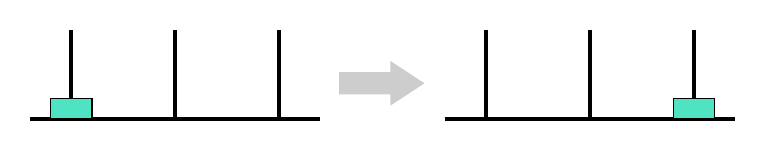
\begin{tikzpicture}[x=0.75pt,y=0.75pt,yscale=-1,xscale=1]
%uncomment if require: \path (0,387); %set diagram left start at 0, and has height of 387

%Straight Lines [id:da40902814921476005] 
\draw [line width=1.5]    (0,43) -- (140,43) ;
%Straight Lines [id:da32687008830530373] 
\draw [line width=1.5]    (20,43) -- (20,0) ;
%Straight Lines [id:da3172525661879657] 
\draw [line width=1.5]    (70,43) -- (70,0) ;
%Straight Lines [id:da3724427659815115] 
\draw [line width=1.5]    (120,43) -- (120,0) ;
%Shape: Rectangle [id:dp12926306550885913] 
\draw  [fill={rgb, 255:red, 80; green, 227; blue, 194 }  ,fill opacity=1 ] (10,33) -- (30,33) -- (30,43) -- (10,43) -- cycle ;
%Straight Lines [id:da944371051878028] 
\draw [line width=1.5]    (200,43) -- (340,43) ;
%Straight Lines [id:da5623860802403418] 
\draw [line width=1.5]    (220,43) -- (220,0) ;
%Straight Lines [id:da9847294698370319] 
\draw [line width=1.5]    (270,43) -- (270,0) ;
%Straight Lines [id:da7330741622812829] 
\draw [line width=1.5]    (320,43) -- (320,0) ;
%Shape: Rectangle [id:dp6766108174560563] 
\draw  [fill={rgb, 255:red, 80; green, 227; blue, 194 }  ,fill opacity=1 ] (310,33) -- (330,33) -- (330,43) -- (310,43) -- cycle ;
%Right Arrow [id:dp9017051385213559] 
\draw  [draw opacity=0][fill={rgb, 255:red, 155; green, 155; blue, 155 }  ,fill opacity=0.5 ] (149,20.4) -- (173.71,20.4) -- (173.71,15) -- (190.18,25.8) -- (173.71,36.59) -- (173.71,31.19) -- (149,31.19) -- cycle ;




\end{tikzpicture}
    \caption{The solution of the Tower of Pell with $n=1$ discs.}
\end{figure}

\begin{figure}[H]
    \centering
    

\tikzset{every picture/.style={line width=0.75pt}} %set default line width to 0.75pt        

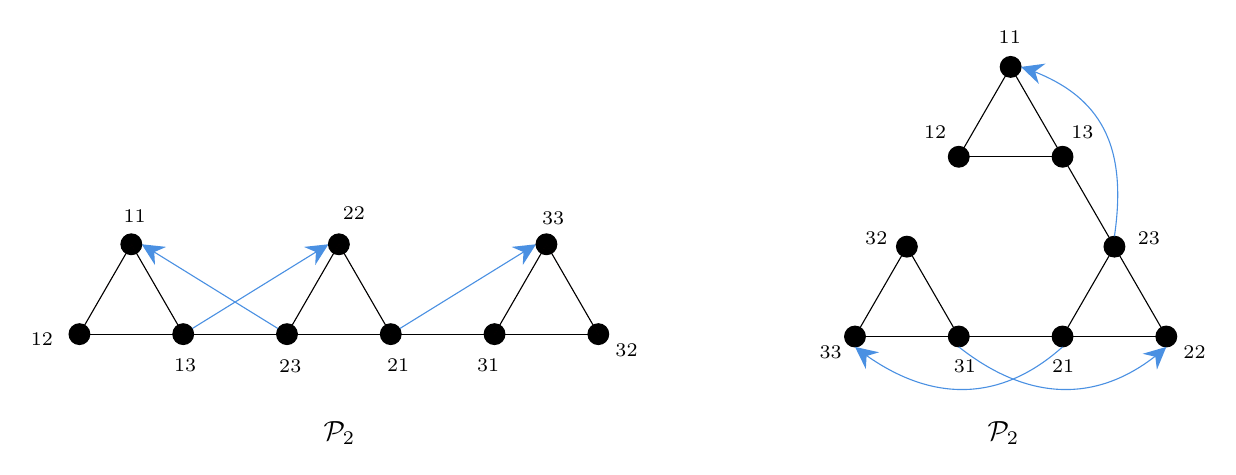
\begin{tikzpicture}[x=0.75pt,y=0.75pt,yscale=-1,xscale=1]
%uncomment if require: \path (0,548); %set diagram left start at 0, and has height of 548

%Straight Lines [id:da6901507393682651] 
\draw    (449.33,78.24) -- (499.33,78.24) ;
%Straight Lines [id:da21446732644725697] 
\draw    (474.33,34.94) -- (499.33,78.24) ;
%Straight Lines [id:da37993334561520187] 
\draw    (474.33,34.94) -- (449.33,78.24) ;
%Shape: Circle [id:dp8863978038112332] 
\draw  [fill={rgb, 255:red, 0; green, 0; blue, 0 }  ,fill opacity=1 ] (469.33,34.94) .. controls (469.33,32.18) and (471.57,29.94) .. (474.33,29.94) .. controls (477.09,29.94) and (479.33,32.18) .. (479.33,34.94) .. controls (479.33,37.7) and (477.09,39.94) .. (474.33,39.94) .. controls (471.57,39.94) and (469.33,37.7) .. (469.33,34.94) -- cycle ;
%Shape: Circle [id:dp5586177169614879] 
\draw  [fill={rgb, 255:red, 0; green, 0; blue, 0 }  ,fill opacity=1 ] (444.33,78.24) .. controls (444.33,75.48) and (446.57,73.24) .. (449.33,73.24) .. controls (452.09,73.24) and (454.33,75.48) .. (454.33,78.24) .. controls (454.33,81) and (452.09,83.24) .. (449.33,83.24) .. controls (446.57,83.24) and (444.33,81) .. (444.33,78.24) -- cycle ;
%Shape: Circle [id:dp3791143954276188] 
\draw  [fill={rgb, 255:red, 0; green, 0; blue, 0 }  ,fill opacity=1 ] (494.33,78.24) .. controls (494.33,75.48) and (496.57,73.24) .. (499.33,73.24) .. controls (502.09,73.24) and (504.33,75.48) .. (504.33,78.24) .. controls (504.33,81) and (502.09,83.24) .. (499.33,83.24) .. controls (496.57,83.24) and (494.33,81) .. (494.33,78.24) -- cycle ;
%Straight Lines [id:da5382832771878143] 
\draw    (424.33,121.54) -- (399.33,164.84) ;
%Straight Lines [id:da9256914873751654] 
\draw    (499.33,78.24) -- (524.33,121.54) ;
%Straight Lines [id:da8970350625801684] 
\draw    (524.33,121.54) -- (549.33,164.84) ;
%Straight Lines [id:da6737612062817164] 
\draw    (524.33,121.54) -- (499.33,164.84) ;
%Straight Lines [id:da9675442867143569] 
\draw    (424.33,121.54) -- (449.33,164.84) ;
%Straight Lines [id:da32775366686998075] 
\draw    (399.33,164.84) -- (449.33,164.84) ;
%Straight Lines [id:da8348135286384326] 
\draw    (499.33,164.84) -- (549.33,164.84) ;
%Straight Lines [id:da9883496143552655] 
\draw    (449.33,164.84) -- (499.33,164.84) ;
%Shape: Circle [id:dp5492856074993371] 
\draw  [fill={rgb, 255:red, 0; green, 0; blue, 0 }  ,fill opacity=1 ] (544.33,164.84) .. controls (544.33,162.08) and (546.57,159.84) .. (549.33,159.84) .. controls (552.09,159.84) and (554.33,162.08) .. (554.33,164.84) .. controls (554.33,167.61) and (552.09,169.84) .. (549.33,169.84) .. controls (546.57,169.84) and (544.33,167.61) .. (544.33,164.84) -- cycle ;
%Shape: Circle [id:dp36554457808583884] 
\draw  [fill={rgb, 255:red, 0; green, 0; blue, 0 }  ,fill opacity=1 ] (494.33,164.84) .. controls (494.33,162.08) and (496.57,159.84) .. (499.33,159.84) .. controls (502.09,159.84) and (504.33,162.08) .. (504.33,164.84) .. controls (504.33,167.61) and (502.09,169.84) .. (499.33,169.84) .. controls (496.57,169.84) and (494.33,167.61) .. (494.33,164.84) -- cycle ;
%Shape: Circle [id:dp203243481486455] 
\draw  [fill={rgb, 255:red, 0; green, 0; blue, 0 }  ,fill opacity=1 ] (519.33,121.54) .. controls (519.33,118.78) and (521.57,116.54) .. (524.33,116.54) .. controls (527.09,116.54) and (529.33,118.78) .. (529.33,121.54) .. controls (529.33,124.31) and (527.09,126.54) .. (524.33,126.54) .. controls (521.57,126.54) and (519.33,124.31) .. (519.33,121.54) -- cycle ;
%Shape: Circle [id:dp5737018031327124] 
\draw  [fill={rgb, 255:red, 0; green, 0; blue, 0 }  ,fill opacity=1 ] (444.33,164.84) .. controls (444.33,162.08) and (446.57,159.84) .. (449.33,159.84) .. controls (452.09,159.84) and (454.33,162.08) .. (454.33,164.84) .. controls (454.33,167.61) and (452.09,169.84) .. (449.33,169.84) .. controls (446.57,169.84) and (444.33,167.61) .. (444.33,164.84) -- cycle ;
%Shape: Circle [id:dp7751149247918085] 
\draw  [fill={rgb, 255:red, 0; green, 0; blue, 0 }  ,fill opacity=1 ] (394.33,164.84) .. controls (394.33,162.08) and (396.57,159.84) .. (399.33,159.84) .. controls (402.09,159.84) and (404.33,162.08) .. (404.33,164.84) .. controls (404.33,167.61) and (402.09,169.84) .. (399.33,169.84) .. controls (396.57,169.84) and (394.33,167.61) .. (394.33,164.84) -- cycle ;
%Shape: Circle [id:dp9546898160285104] 
\draw  [fill={rgb, 255:red, 0; green, 0; blue, 0 }  ,fill opacity=1 ] (419.33,121.54) .. controls (419.33,118.78) and (421.57,116.54) .. (424.33,116.54) .. controls (427.09,116.54) and (429.33,118.78) .. (429.33,121.54) .. controls (429.33,124.31) and (427.09,126.54) .. (424.33,126.54) .. controls (421.57,126.54) and (419.33,124.31) .. (419.33,121.54) -- cycle ;
%Curve Lines [id:da4707171071996783] 
\draw [color={rgb, 255:red, 74; green, 144; blue, 226 }  ,draw opacity=1 ]   (482.71,36.1) .. controls (518.38,48.94) and (530.64,73.33) .. (524.33,116.54) ;
\draw [shift={(479.33,34.94)}, rotate = 18.1] [fill={rgb, 255:red, 74; green, 144; blue, 226 }  ,fill opacity=1 ][line width=0.08]  [draw opacity=0] (10.72,-5.15) -- (0,0) -- (10.72,5.15) -- (7.12,0) -- cycle    ;
%Curve Lines [id:da6374523862436225] 
\draw [color={rgb, 255:red, 74; green, 144; blue, 226 }  ,draw opacity=1 ]   (499.33,169.84) .. controls (469.96,196.2) and (436.05,197.7) .. (401.45,171.48) ;
\draw [shift={(399.33,169.84)}, rotate = 38.3] [fill={rgb, 255:red, 74; green, 144; blue, 226 }  ,fill opacity=1 ][line width=0.08]  [draw opacity=0] (10.72,-5.15) -- (0,0) -- (10.72,5.15) -- (7.12,0) -- cycle    ;
%Curve Lines [id:da5150906259303378] 
\draw [color={rgb, 255:red, 74; green, 144; blue, 226 }  ,draw opacity=1 ]   (546.62,172.2) .. controls (517.28,196.77) and (483.6,196.91) .. (449.33,169.84) ;
\draw [shift={(549.33,169.84)}, rotate = 138.1] [fill={rgb, 255:red, 74; green, 144; blue, 226 }  ,fill opacity=1 ][line width=0.08]  [draw opacity=0] (10.72,-5.15) -- (0,0) -- (10.72,5.15) -- (7.12,0) -- cycle    ;

%Straight Lines [id:da8695544914737432] 
\draw [color={rgb, 255:red, 74; green, 144; blue, 226 }  ,draw opacity=1 ]   (75.67,163.7) -- (143.12,121.98) ;
\draw [shift={(145.67,120.4)}, rotate = 148.26] [fill={rgb, 255:red, 74; green, 144; blue, 226 }  ,fill opacity=1 ][line width=0.08]  [draw opacity=0] (10.72,-5.15) -- (0,0) -- (10.72,5.15) -- (7.12,0) -- cycle    ;
%Straight Lines [id:da8668725138183859] 
\draw [color={rgb, 255:red, 74; green, 144; blue, 226 }  ,draw opacity=1 ]   (125.67,163.7) -- (58.22,121.98) ;
\draw [shift={(55.67,120.4)}, rotate = 31.74] [fill={rgb, 255:red, 74; green, 144; blue, 226 }  ,fill opacity=1 ][line width=0.08]  [draw opacity=0] (10.72,-5.15) -- (0,0) -- (10.72,5.15) -- (7.12,0) -- cycle    ;
%Straight Lines [id:da16107120099277372] 
\draw [color={rgb, 255:red, 74; green, 144; blue, 226 }  ,draw opacity=1 ]   (175.67,163.7) -- (243.12,121.98) ;
\draw [shift={(245.67,120.4)}, rotate = 148.26] [fill={rgb, 255:red, 74; green, 144; blue, 226 }  ,fill opacity=1 ][line width=0.08]  [draw opacity=0] (10.72,-5.15) -- (0,0) -- (10.72,5.15) -- (7.12,0) -- cycle    ;
%Shape: Circle [id:dp8937463835396178] 
\draw  [fill={rgb, 255:red, 0; green, 0; blue, 0 }  ,fill opacity=1 ] (45.67,120.4) .. controls (45.67,117.64) and (47.91,115.4) .. (50.67,115.4) .. controls (53.43,115.4) and (55.67,117.64) .. (55.67,120.4) .. controls (55.67,123.16) and (53.43,125.4) .. (50.67,125.4) .. controls (47.91,125.4) and (45.67,123.16) .. (45.67,120.4) -- cycle ;
%Shape: Circle [id:dp44810172880860777] 
\draw  [fill={rgb, 255:red, 0; green, 0; blue, 0 }  ,fill opacity=1 ] (20.67,163.7) .. controls (20.67,160.94) and (22.91,158.7) .. (25.67,158.7) .. controls (28.43,158.7) and (30.67,160.94) .. (30.67,163.7) .. controls (30.67,166.46) and (28.43,168.7) .. (25.67,168.7) .. controls (22.91,168.7) and (20.67,166.46) .. (20.67,163.7) -- cycle ;
%Straight Lines [id:da6507317055589545] 
\draw [fill={rgb, 255:red, 208; green, 2; blue, 27 }  ,fill opacity=1 ]   (25.67,163.7) -- (75.67,163.7) ;
%Shape: Circle [id:dp8523058956784781] 
\draw  [fill={rgb, 255:red, 0; green, 0; blue, 0 }  ,fill opacity=1 ] (70.67,163.7) .. controls (70.67,160.94) and (72.91,158.7) .. (75.67,158.7) .. controls (78.43,158.7) and (80.67,160.94) .. (80.67,163.7) .. controls (80.67,166.46) and (78.43,168.7) .. (75.67,168.7) .. controls (72.91,168.7) and (70.67,166.46) .. (70.67,163.7) -- cycle ;
%Straight Lines [id:da3754427566815943] 
\draw [fill={rgb, 255:red, 208; green, 2; blue, 27 }  ,fill opacity=1 ]   (50.67,120.4) -- (25.67,163.7) ;
%Straight Lines [id:da5842523797117667] 
\draw [fill={rgb, 255:red, 208; green, 2; blue, 27 }  ,fill opacity=1 ]   (50.67,120.4) -- (75.67,163.7) ;
%Straight Lines [id:da73292664353717] 
\draw    (75.67,163.7) -- (125.67,163.7) ;
%Shape: Circle [id:dp6081318508915146] 
\draw  [fill={rgb, 255:red, 0; green, 0; blue, 0 }  ,fill opacity=1 ] (120.67,163.7) .. controls (120.67,160.94) and (122.91,158.7) .. (125.67,158.7) .. controls (128.43,158.7) and (130.67,160.94) .. (130.67,163.7) .. controls (130.67,166.46) and (128.43,168.7) .. (125.67,168.7) .. controls (122.91,168.7) and (120.67,166.46) .. (120.67,163.7) -- cycle ;
%Straight Lines [id:da21809054531931316] 
\draw    (125.67,163.7) -- (175.67,163.7) ;
%Shape: Circle [id:dp6620599054856162] 
\draw  [fill={rgb, 255:red, 0; green, 0; blue, 0 }  ,fill opacity=1 ] (170.67,163.7) .. controls (170.67,160.94) and (172.91,158.7) .. (175.67,158.7) .. controls (178.43,158.7) and (180.67,160.94) .. (180.67,163.7) .. controls (180.67,166.46) and (178.43,168.7) .. (175.67,168.7) .. controls (172.91,168.7) and (170.67,166.46) .. (170.67,163.7) -- cycle ;
%Straight Lines [id:da16013499644553653] 
\draw    (175.67,163.7) -- (225.67,163.7) ;
%Straight Lines [id:da9663832741334577] 
\draw    (225.67,163.7) -- (275.67,163.7) ;
%Shape: Circle [id:dp14130329886100057] 
\draw  [fill={rgb, 255:red, 0; green, 0; blue, 0 }  ,fill opacity=1 ] (220.67,163.7) .. controls (220.67,160.94) and (222.91,158.7) .. (225.67,158.7) .. controls (228.43,158.7) and (230.67,160.94) .. (230.67,163.7) .. controls (230.67,166.46) and (228.43,168.7) .. (225.67,168.7) .. controls (222.91,168.7) and (220.67,166.46) .. (220.67,163.7) -- cycle ;
%Shape: Circle [id:dp18057656169319558] 
\draw  [fill={rgb, 255:red, 0; green, 0; blue, 0 }  ,fill opacity=1 ] (145.67,120.4) .. controls (145.67,117.64) and (147.91,115.4) .. (150.67,115.4) .. controls (153.43,115.4) and (155.67,117.64) .. (155.67,120.4) .. controls (155.67,123.16) and (153.43,125.4) .. (150.67,125.4) .. controls (147.91,125.4) and (145.67,123.16) .. (145.67,120.4) -- cycle ;
%Straight Lines [id:da4588184949881646] 
\draw [fill={rgb, 255:red, 208; green, 2; blue, 27 }  ,fill opacity=1 ]   (150.67,120.4) -- (125.67,163.7) ;
%Straight Lines [id:da5608318843258293] 
\draw [fill={rgb, 255:red, 208; green, 2; blue, 27 }  ,fill opacity=1 ]   (150.67,120.4) -- (175.67,163.7) ;
%Shape: Circle [id:dp5187668713593079] 
\draw  [fill={rgb, 255:red, 0; green, 0; blue, 0 }  ,fill opacity=1 ] (270.67,163.7) .. controls (270.67,160.94) and (272.91,158.7) .. (275.67,158.7) .. controls (278.43,158.7) and (280.67,160.94) .. (280.67,163.7) .. controls (280.67,166.46) and (278.43,168.7) .. (275.67,168.7) .. controls (272.91,168.7) and (270.67,166.46) .. (270.67,163.7) -- cycle ;
%Shape: Circle [id:dp06384022562571845] 
\draw  [fill={rgb, 255:red, 0; green, 0; blue, 0 }  ,fill opacity=1 ] (245.67,120.4) .. controls (245.67,117.64) and (247.91,115.4) .. (250.67,115.4) .. controls (253.43,115.4) and (255.67,117.64) .. (255.67,120.4) .. controls (255.67,123.16) and (253.43,125.4) .. (250.67,125.4) .. controls (247.91,125.4) and (245.67,123.16) .. (245.67,120.4) -- cycle ;
%Straight Lines [id:da19105310945203935] 
\draw [fill={rgb, 255:red, 208; green, 2; blue, 27 }  ,fill opacity=1 ]   (250.67,120.4) -- (225.67,163.7) ;
%Straight Lines [id:da701352664831173] 
\draw [fill={rgb, 255:red, 208; green, 2; blue, 27 }  ,fill opacity=1 ]   (250.67,120.4) -- (275.67,163.7) ;


% Text Node
\draw (1,161.73) node [anchor=north west][inner sep=0.75pt]  [font=\scriptsize]  {$12$};
% Text Node
\draw (120.67,175.07) node [anchor=north west][inner sep=0.75pt]  [font=\scriptsize]  {$23$};
% Text Node
\draw (45.67,102.73) node [anchor=north west][inner sep=0.75pt]  [font=\scriptsize]  {$11$};
% Text Node
\draw (70,174.4) node [anchor=north west][inner sep=0.75pt]  [font=\scriptsize]  {$13$};
% Text Node
\draw (151.33,101.07) node [anchor=north west][inner sep=0.75pt]  [font=\scriptsize]  {$22$};
% Text Node
\draw (172.67,174.34) node [anchor=north west][inner sep=0.75pt]  [font=\scriptsize]  {$21$};
% Text Node
\draw (216,174.34) node [anchor=north west][inner sep=0.75pt]  [font=\scriptsize]  {$31$};
% Text Node
\draw (282.67,167.1) node [anchor=north west][inner sep=0.75pt]  [font=\scriptsize]  {$32$};
% Text Node
\draw (247.33,103.73) node [anchor=north west][inner sep=0.75pt]  [font=\scriptsize]  {$33$};
% Text Node
\draw (467.33,16.31) node [anchor=north west][inner sep=0.75pt]  [font=\scriptsize]  {$11$};
% Text Node
\draw (556.33,168.31) node [anchor=north west][inner sep=0.75pt]  [font=\scriptsize]  {$22$};
% Text Node
\draw (381,168.31) node [anchor=north west][inner sep=0.75pt]  [font=\scriptsize]  {$33$};
% Text Node
\draw (502.33,62.31) node [anchor=north west][inner sep=0.75pt]  [font=\scriptsize]  {$13$};
% Text Node
\draw (431.33,62.31) node [anchor=north west][inner sep=0.75pt]  [font=\scriptsize]  {$12$};
% Text Node
\draw (493,174.91) node [anchor=north west][inner sep=0.75pt]  [font=\scriptsize]  {$21$};
% Text Node
\draw (534.33,113.31) node [anchor=north west][inner sep=0.75pt]  [font=\scriptsize]  {$23$};
% Text Node
\draw (445.67,174.91) node [anchor=north west][inner sep=0.75pt]  [font=\scriptsize]  {$31$};
% Text Node
\draw (403,113.31) node [anchor=north west][inner sep=0.75pt]  [font=\scriptsize]  {$32$};
% Text Node
\draw (142,204.4) node [anchor=north west][inner sep=0.75pt]    {$\mathcal{P}_{2}$};
% Text Node
\draw (462,204.4) node [anchor=north west][inner sep=0.75pt]    {$\mathcal{P}_{2}$};


\end{tikzpicture}
    \caption{The solution of the Tower of Pell with $n=2$ discs.}
\end{figure}

\begin{figure}[H]
    \centering
    

\tikzset{every picture/.style={line width=0.75pt}} %set default line width to 0.75pt        

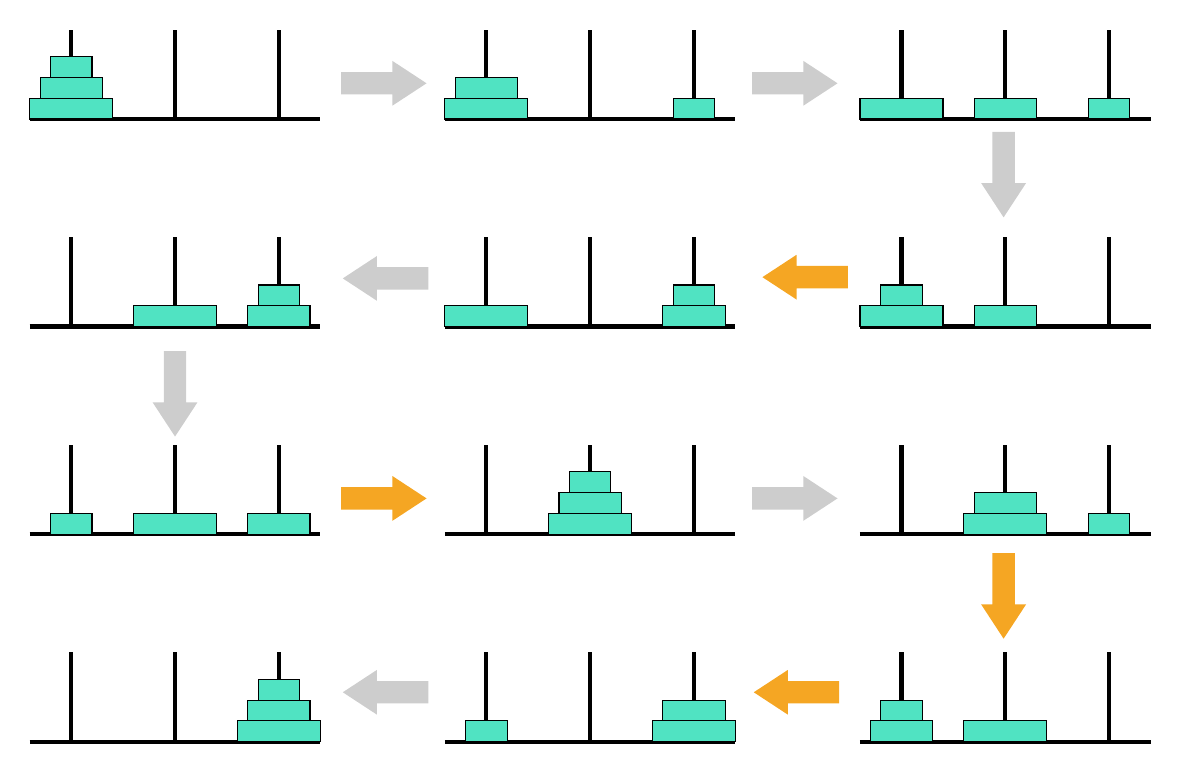
\begin{tikzpicture}[x=0.75pt,y=0.75pt,yscale=-1,xscale=1]
%uncomment if require: \path (0,450); %set diagram left start at 0, and has height of 450

%Straight Lines [id:da03223376237952125] 
\draw [line width=1.5]    (0,43) -- (140,43) ;
%Straight Lines [id:da6275309772911721] 
\draw [line width=1.5]    (20,43) -- (20,0) ;
%Straight Lines [id:da5948161113195467] 
\draw [line width=1.5]    (70,43) -- (70,0) ;
%Straight Lines [id:da7203610541938157] 
\draw [line width=1.5]    (120,43) -- (120,0) ;
%Shape: Rectangle [id:dp20286334481080437] 
\draw  [fill={rgb, 255:red, 80; green, 227; blue, 194 }  ,fill opacity=1 ] (10,13) -- (30,13) -- (30,23) -- (10,23) -- cycle ;
%Shape: Rectangle [id:dp1430532555535371] 
\draw  [fill={rgb, 255:red, 80; green, 227; blue, 194 }  ,fill opacity=1 ] (5,23) -- (35,23) -- (35,33) -- (5,33) -- cycle ;
%Shape: Rectangle [id:dp18658521432006636] 
\draw  [fill={rgb, 255:red, 80; green, 227; blue, 194 }  ,fill opacity=1 ] (0,33) -- (40,33) -- (40,43) -- (0,43) -- cycle ;
%Right Arrow [id:dp1572741433487066] 
\draw  [draw opacity=0][fill={rgb, 255:red, 155; green, 155; blue, 155 }  ,fill opacity=0.5 ] (150,20.4) -- (174.71,20.4) -- (174.71,15) -- (191.18,25.8) -- (174.71,36.59) -- (174.71,31.19) -- (150,31.19) -- cycle ;
%Straight Lines [id:da9240432629260678] 
\draw [line width=1.5]    (200,43) -- (340,43) ;
%Straight Lines [id:da5339882365373494] 
\draw [line width=1.5]    (220,43) -- (220,0) ;
%Straight Lines [id:da5853661233119658] 
\draw [line width=1.5]    (270,43) -- (270,0) ;
%Straight Lines [id:da2909185099712355] 
\draw [line width=1.5]    (320,43) -- (320,0) ;
%Shape: Rectangle [id:dp8621683135066898] 
\draw  [fill={rgb, 255:red, 80; green, 227; blue, 194 }  ,fill opacity=1 ] (310,33) -- (330,33) -- (330,43) -- (310,43) -- cycle ;
%Shape: Rectangle [id:dp21037908042057096] 
\draw  [fill={rgb, 255:red, 80; green, 227; blue, 194 }  ,fill opacity=1 ] (205,23) -- (235,23) -- (235,33) -- (205,33) -- cycle ;
%Shape: Rectangle [id:dp08358955198875151] 
\draw  [fill={rgb, 255:red, 80; green, 227; blue, 194 }  ,fill opacity=1 ] (200,33) -- (240,33) -- (240,43) -- (200,43) -- cycle ;
%Straight Lines [id:da23677295851965852] 
\draw [line width=1.5]    (400,43) -- (540,43) ;
%Straight Lines [id:da5901115792892262] 
\draw [line width=1.5]    (420,43) -- (420,0) ;
%Straight Lines [id:da45160565900836613] 
\draw [line width=1.5]    (470,43) -- (470,0) ;
%Straight Lines [id:da19612966045701197] 
\draw [line width=1.5]    (520,43) -- (520,0) ;
%Shape: Rectangle [id:dp8618896738863524] 
\draw  [fill={rgb, 255:red, 80; green, 227; blue, 194 }  ,fill opacity=1 ] (510,33) -- (530,33) -- (530,43) -- (510,43) -- cycle ;
%Shape: Rectangle [id:dp7242550067493401] 
\draw  [fill={rgb, 255:red, 80; green, 227; blue, 194 }  ,fill opacity=1 ] (455,33) -- (485,33) -- (485,43) -- (455,43) -- cycle ;
%Shape: Rectangle [id:dp2814756844944881] 
\draw  [fill={rgb, 255:red, 80; green, 227; blue, 194 }  ,fill opacity=1 ] (400,33) -- (440,33) -- (440,43) -- (400,43) -- cycle ;
%Straight Lines [id:da3096488327187181] 
\draw [line width=1.5]    (400,143) -- (540,143) ;
%Straight Lines [id:da26193179763109] 
\draw [line width=1.5]    (420,143) -- (420,100) ;
%Straight Lines [id:da344772974050781] 
\draw [line width=1.5]    (470,143) -- (470,100) ;
%Straight Lines [id:da21731259531086589] 
\draw [line width=1.5]    (520,143) -- (520,100) ;
%Shape: Rectangle [id:dp7699113688324271] 
\draw  [fill={rgb, 255:red, 80; green, 227; blue, 194 }  ,fill opacity=1 ] (410,123) -- (430,123) -- (430,133) -- (410,133) -- cycle ;
%Shape: Rectangle [id:dp8086660195801876] 
\draw  [fill={rgb, 255:red, 80; green, 227; blue, 194 }  ,fill opacity=1 ] (455,133) -- (485,133) -- (485,143) -- (455,143) -- cycle ;
%Shape: Rectangle [id:dp5382115262699121] 
\draw  [fill={rgb, 255:red, 80; green, 227; blue, 194 }  ,fill opacity=1 ] (400,133) -- (440,133) -- (440,143) -- (400,143) -- cycle ;
%Straight Lines [id:da6777668709508031] 
\draw [line width=1.5]    (200,143) -- (340,143) ;
%Straight Lines [id:da7154296393750508] 
\draw [line width=1.5]    (220,143) -- (220,100) ;
%Straight Lines [id:da23290492651700556] 
\draw [line width=1.5]    (270,143) -- (270,100) ;
%Straight Lines [id:da6459086136379697] 
\draw [line width=1.5]    (320,143) -- (320,100) ;
%Shape: Rectangle [id:dp09203833774233972] 
\draw  [fill={rgb, 255:red, 80; green, 227; blue, 194 }  ,fill opacity=1 ] (310,123) -- (330,123) -- (330,133) -- (310,133) -- cycle ;
%Shape: Rectangle [id:dp5640564126439245] 
\draw  [fill={rgb, 255:red, 80; green, 227; blue, 194 }  ,fill opacity=1 ] (305,133) -- (335,133) -- (335,143) -- (305,143) -- cycle ;
%Shape: Rectangle [id:dp2097253437843838] 
\draw  [fill={rgb, 255:red, 80; green, 227; blue, 194 }  ,fill opacity=1 ] (200,133) -- (240,133) -- (240,143) -- (200,143) -- cycle ;
%Straight Lines [id:da8477188501614394] 
\draw [line width=1.5]    (0,143) -- (140,143) ;
%Straight Lines [id:da6310455745903174] 
\draw [line width=1.5]    (20,143) -- (20,100) ;
%Straight Lines [id:da8794404983838642] 
\draw [line width=1.5]    (70,143) -- (70,100) ;
%Straight Lines [id:da9287811133172703] 
\draw [line width=1.5]    (120,143) -- (120,100) ;
%Shape: Rectangle [id:dp13466408039451827] 
\draw  [fill={rgb, 255:red, 80; green, 227; blue, 194 }  ,fill opacity=1 ] (110,123) -- (130,123) -- (130,133) -- (110,133) -- cycle ;
%Shape: Rectangle [id:dp8749306277728901] 
\draw  [fill={rgb, 255:red, 80; green, 227; blue, 194 }  ,fill opacity=1 ] (105,133) -- (135,133) -- (135,143) -- (105,143) -- cycle ;
%Shape: Rectangle [id:dp8138890479919696] 
\draw  [fill={rgb, 255:red, 80; green, 227; blue, 194 }  ,fill opacity=1 ] (50,133) -- (90,133) -- (90,143) -- (50,143) -- cycle ;
%Straight Lines [id:da2219579401463203] 
\draw [line width=1.5]    (0,243) -- (140,243) ;
%Straight Lines [id:da6651670929291789] 
\draw [line width=1.5]    (20,243) -- (20,200) ;
%Straight Lines [id:da31312844282951824] 
\draw [line width=1.5]    (70,243) -- (70,200) ;
%Straight Lines [id:da2011595708863807] 
\draw [line width=1.5]    (120,243) -- (120,200) ;
%Shape: Rectangle [id:dp4996621742610865] 
\draw  [fill={rgb, 255:red, 80; green, 227; blue, 194 }  ,fill opacity=1 ] (10,233) -- (30,233) -- (30,243) -- (10,243) -- cycle ;
%Shape: Rectangle [id:dp1608999248828069] 
\draw  [fill={rgb, 255:red, 80; green, 227; blue, 194 }  ,fill opacity=1 ] (105,233) -- (135,233) -- (135,243) -- (105,243) -- cycle ;
%Shape: Rectangle [id:dp5855101063984169] 
\draw  [fill={rgb, 255:red, 80; green, 227; blue, 194 }  ,fill opacity=1 ] (50,233) -- (90,233) -- (90,243) -- (50,243) -- cycle ;
%Straight Lines [id:da32600659389166786] 
\draw [line width=1.5]    (200,243) -- (340,243) ;
%Straight Lines [id:da4394322223179583] 
\draw [line width=1.5]    (220,243) -- (220,200) ;
%Straight Lines [id:da8697277296703456] 
\draw [line width=1.5]    (270,243) -- (270,200) ;
%Straight Lines [id:da9909761340387837] 
\draw [line width=1.5]    (320,243) -- (320,200) ;
%Shape: Rectangle [id:dp10133245349806397] 
\draw  [fill={rgb, 255:red, 80; green, 227; blue, 194 }  ,fill opacity=1 ] (260,213) -- (280,213) -- (280,223) -- (260,223) -- cycle ;
%Shape: Rectangle [id:dp12221777208045381] 
\draw  [fill={rgb, 255:red, 80; green, 227; blue, 194 }  ,fill opacity=1 ] (255,223) -- (285,223) -- (285,233) -- (255,233) -- cycle ;
%Shape: Rectangle [id:dp18680896303692784] 
\draw  [fill={rgb, 255:red, 80; green, 227; blue, 194 }  ,fill opacity=1 ] (250,233) -- (290,233) -- (290,243) -- (250,243) -- cycle ;
%Right Arrow [id:dp11972371824411421] 
\draw  [draw opacity=0][fill={rgb, 255:red, 155; green, 155; blue, 155 }  ,fill opacity=0.5 ] (348,20.4) -- (372.71,20.4) -- (372.71,15) -- (389.18,25.8) -- (372.71,36.59) -- (372.71,31.19) -- (348,31.19) -- cycle ;
%Right Arrow [id:dp5323868973546051] 
\draw  [draw opacity=0][fill={rgb, 255:red, 155; green, 155; blue, 155 }  ,fill opacity=0.5 ] (474.6,49.2) -- (474.6,73.91) -- (480,73.91) -- (469.2,90.39) -- (458.41,73.91) -- (463.81,73.91) -- (463.81,49.2) -- cycle ;
%Right Arrow [id:dp3479249707227101] 
\draw  [draw opacity=0][fill={rgb, 255:red, 245; green, 166; blue, 35 }  ,fill opacity=1 ] (394.18,124.6) -- (369.47,124.6) -- (369.47,130) -- (353,119.2) -- (369.47,108.41) -- (369.47,113.81) -- (394.18,113.81) -- cycle ;
%Right Arrow [id:dp5108040776629461] 
\draw  [draw opacity=0][fill={rgb, 255:red, 155; green, 155; blue, 155 }  ,fill opacity=0.5 ] (192,125.19) -- (167.29,125.19) -- (167.29,130.59) -- (150.82,119.8) -- (167.29,109) -- (167.29,114.4) -- (192,114.4) -- cycle ;
%Right Arrow [id:dp4431168559788772] 
\draw  [draw opacity=0][fill={rgb, 255:red, 155; green, 155; blue, 155 }  ,fill opacity=0.5 ] (75.4,154.82) -- (75.4,179.53) -- (80.8,179.53) -- (70,196) -- (59.2,179.53) -- (64.6,179.53) -- (64.6,154.82) -- cycle ;
%Right Arrow [id:dp6336454391535531] 
\draw  [draw opacity=0][fill={rgb, 255:red, 245; green, 166; blue, 35 }  ,fill opacity=1 ] (150,220.4) -- (174.71,220.4) -- (174.71,215) -- (191.18,225.8) -- (174.71,236.59) -- (174.71,231.19) -- (150,231.19) -- cycle ;
%Straight Lines [id:da7183373068521042] 
\draw [line width=1.5]    (400,243) -- (540,243) ;
%Straight Lines [id:da17113292702937222] 
\draw [line width=1.5]    (420,243) -- (420,200) ;
%Straight Lines [id:da4926491837061766] 
\draw [line width=1.5]    (470,243) -- (470,200) ;
%Straight Lines [id:da3895378366177431] 
\draw [line width=1.5]    (520,243) -- (520,200) ;
%Shape: Rectangle [id:dp6194781675886842] 
\draw  [fill={rgb, 255:red, 80; green, 227; blue, 194 }  ,fill opacity=1 ] (510,233) -- (530,233) -- (530,243) -- (510,243) -- cycle ;
%Shape: Rectangle [id:dp24846944338981092] 
\draw  [fill={rgb, 255:red, 80; green, 227; blue, 194 }  ,fill opacity=1 ] (455,223) -- (485,223) -- (485,233) -- (455,233) -- cycle ;
%Shape: Rectangle [id:dp8872343609913609] 
\draw  [fill={rgb, 255:red, 80; green, 227; blue, 194 }  ,fill opacity=1 ] (450,233) -- (490,233) -- (490,243) -- (450,243) -- cycle ;
%Right Arrow [id:dp8158012395961658] 
\draw  [draw opacity=0][fill={rgb, 255:red, 155; green, 155; blue, 155 }  ,fill opacity=0.5 ] (348,220.4) -- (372.71,220.4) -- (372.71,215) -- (389.18,225.8) -- (372.71,236.59) -- (372.71,231.19) -- (348,231.19) -- cycle ;
%Straight Lines [id:da22197097301087987] 
\draw [line width=1.5]    (400,343) -- (540,343) ;
%Straight Lines [id:da5499508796113233] 
\draw [line width=1.5]    (420,343) -- (420,300) ;
%Straight Lines [id:da727330095208504] 
\draw [line width=1.5]    (470,343) -- (470,300) ;
%Straight Lines [id:da24354958936332527] 
\draw [line width=1.5]    (520,343) -- (520,300) ;
%Shape: Rectangle [id:dp9639472303360237] 
\draw  [fill={rgb, 255:red, 80; green, 227; blue, 194 }  ,fill opacity=1 ] (410,323) -- (430,323) -- (430,333) -- (410,333) -- cycle ;
%Shape: Rectangle [id:dp057818147501542905] 
\draw  [fill={rgb, 255:red, 80; green, 227; blue, 194 }  ,fill opacity=1 ] (405,333) -- (435,333) -- (435,343) -- (405,343) -- cycle ;
%Shape: Rectangle [id:dp8298046795652936] 
\draw  [fill={rgb, 255:red, 80; green, 227; blue, 194 }  ,fill opacity=1 ] (450,333) -- (490,333) -- (490,343) -- (450,343) -- cycle ;
%Right Arrow [id:dp969249735538718] 
\draw  [draw opacity=0][fill={rgb, 255:red, 245; green, 166; blue, 35 }  ,fill opacity=1 ] (474.6,252.2) -- (474.6,276.91) -- (480,276.91) -- (469.2,293.39) -- (458.41,276.91) -- (463.81,276.91) -- (463.81,252.2) -- cycle ;
%Straight Lines [id:da26757493226265194] 
\draw [line width=1.5]    (200,343) -- (340,343) ;
%Straight Lines [id:da12340162972623481] 
\draw [line width=1.5]    (220,343) -- (220,300) ;
%Straight Lines [id:da012115400723181402] 
\draw [line width=1.5]    (270,343) -- (270,300) ;
%Straight Lines [id:da5659423528401684] 
\draw [line width=1.5]    (320,343) -- (320,300) ;
%Shape: Rectangle [id:dp47397910555923506] 
\draw  [fill={rgb, 255:red, 80; green, 227; blue, 194 }  ,fill opacity=1 ] (210,333) -- (230,333) -- (230,343) -- (210,343) -- cycle ;
%Shape: Rectangle [id:dp24721155641257742] 
\draw  [fill={rgb, 255:red, 80; green, 227; blue, 194 }  ,fill opacity=1 ] (305,323) -- (335,323) -- (335,333) -- (305,333) -- cycle ;
%Shape: Rectangle [id:dp9500298151596387] 
\draw  [fill={rgb, 255:red, 80; green, 227; blue, 194 }  ,fill opacity=1 ] (300,333) -- (340,333) -- (340,343) -- (300,343) -- cycle ;
%Right Arrow [id:dp31315664061482584] 
\draw  [draw opacity=0][fill={rgb, 255:red, 245; green, 166; blue, 35 }  ,fill opacity=1 ] (390,324.6) -- (365.29,324.6) -- (365.29,330) -- (348.82,319.2) -- (365.29,308.41) -- (365.29,313.81) -- (390,313.81) -- cycle ;
%Straight Lines [id:da7342018104145998] 
\draw [line width=1.5]    (0,343) -- (140,343) ;
%Straight Lines [id:da16597547039803184] 
\draw [line width=1.5]    (20,343) -- (20,300) ;
%Straight Lines [id:da2832672414615689] 
\draw [line width=1.5]    (70,343) -- (70,300) ;
%Straight Lines [id:da5661454135983732] 
\draw [line width=1.5]    (120,343) -- (120,300) ;
%Shape: Rectangle [id:dp3896149079509228] 
\draw  [fill={rgb, 255:red, 80; green, 227; blue, 194 }  ,fill opacity=1 ] (110,313) -- (130,313) -- (130,323) -- (110,323) -- cycle ;
%Shape: Rectangle [id:dp754408621439774] 
\draw  [fill={rgb, 255:red, 80; green, 227; blue, 194 }  ,fill opacity=1 ] (105,323) -- (135,323) -- (135,333) -- (105,333) -- cycle ;
%Shape: Rectangle [id:dp8684461697976968] 
\draw  [fill={rgb, 255:red, 80; green, 227; blue, 194 }  ,fill opacity=1 ] (100,333) -- (140,333) -- (140,343) -- (100,343) -- cycle ;
%Right Arrow [id:dp05789331359099248] 
\draw  [draw opacity=0][fill={rgb, 255:red, 155; green, 155; blue, 155 }  ,fill opacity=0.5 ] (192,324.6) -- (167.29,324.6) -- (167.29,330) -- (150.82,319.2) -- (167.29,308.41) -- (167.29,313.81) -- (192,313.81) -- cycle ;




\end{tikzpicture}
    \caption{The solution of the Tower of Pell with $n=3$ discs.}\label{fig:pell_optimal_solution_3}
\end{figure}

\end{document}
